%%%%%%%%%%%%%%%%%%%%%%%%%%%%%%%%%%%%%%%%%%%%%%%%%%%%%%%%%%%%%%%%%%%%%%%%%%%%%%%%
%												                               %
% 								    PREAMBLE                                   %
%																			   %
%%%%%%%%%%%%%%%%%%%%%%%%%%%%%%%%%%%%%%%%%%%%%%%%%%%%%%%%%%%%%%%%%%%%%%%%%%%%%%%%

%\RequirePackage[english=spanish]{hyphsubst}
\documentclass[a4paper, 10pt, 
			   %showtrims, drafting,
			   %final,
			   twoside, openright
			  ]{memoir}

\newcommand\hmmax{0}
\newcommand\bmmax{0}
\usepackage{sansmath}

\usepackage{polyglossia}
\setmainlanguage{spanish}
\PolyglossiaSetup{spanish}{indentfirst=false}
\setotherlanguage[variant=polytonic]{greek}
\setotherlanguage{english}

\usepackage{fontspec}
\defaultfontfeatures{Ligatures=TeX}%,Scale=MatchLowercase}


%\usepackage{libertine}
\usepackage{mathpazo}             % Latin Modern newtxsf
%\usepackage{lmodern}
%\RequirePackage[light,condensed,math,lf]{iwona}
%\renewcommand{\sfdefault}{Fira Sans}   % Helvetica (phv)

\usepackage[scaled]{beramono} 

%\fontspec{Palatino}
%\defaultfontfeatures{Ligatures=TeX,Scale=MatchLowercase}
%\setmainfont{Palatino}

%\setsansfont{Fira Sans}

%% Select Sans Font Family
%\setsansfont[BoldFont={* Medium}]{Helvetica Neue}
\setsansfont[BoldFont={* Medium}]{Fira Sans}


%\renewcommand\bfdefault{sb}
%\renewcommand{\bfdefault}{sb}
%\DeclareFontShape{\encodingdefault}{\rmdefault}{sb}{n}
%    {<->ssub*\rmdefault/bx/n}{}
%\DeclareFontShape{\encodingdefault}{\rmdefault}{sb}{sl}
%    {<->ssub*\rmdefault/bx/sl}{}

%\setsansfont{Fira Sans}
%\usepackage{libertine}
%\usepackage{mathpazo}

% Load style
\usepackage{style}  

% Document data
%%%%%%%%%%%%%%%%%%%%%%%%%%%%%%%%%%%%%%%%%%%%%%%%%%%%%%%%%%%%%%%%%%%%%%%%%%%%%%%%
%                                                                              %
%                                MAIN TEX FILE                                 %
%                                                                              %
%                                                                              %
%                                                                              %
%                                                                              %
%                                                                              %
%                                                                              %
%%%%%%%%%%%%%%%%%%%%%%%%%%%%%%%%%%%%%%%%%%%%%%%%%%%%%%%%%%%%%%%%%%%%%%%%%%%%%%%%



%\newcommand{\myTitle}{Medida de la fase de oscilación del $\text{B}_{s}$ 
%                      con toda la muestra de LHC$b$\xspace}
%\newcommand{\myTitle}{\textsc{gpu}--based time--dependent angular analysis %
%                      \begingroup
%                      \small $\Bs \rightarrow \Jpsi \antikaon\kaon$%
%                      \endgroup
%                      and systematic uncertainty validation.\xspace}
\newcommand{\myTitle}{Análisis angular dependiente del tiempo para el canal %
                      \begingroup
                      \small $\Bs \rightarrow \Jpsi \antikaon\kaon$%
                      \endgroup
                      basado en \textsc{gpu}
                      y validación de incertidumbres sistemáticas\xspace}
\newcommand{\mySubtitle}{\xspace}
%\newcommand{\myDegree}{Master Thesis on Industrial Mathematics\xspace}
\newcommand{\myDegree}{Trabajo Fin de Máster en Matemática Industrial\xspace}
\newcommand{\myName}{Marcos Romero Lamas\xspace}
\newcommand{\myProf}{Diego Martínez Santos\xspace}
\newcommand{\myOtherProf}{Veronika Georgieva Chobanova\xspace}
\newcommand{\mySupervisor}{Fernando Varas Mérida\xspace}
\newcommand{\myFaculty}{Facultad de Fí­sica\xspace}
\newcommand{\myDepartment}{Departamento de Física de Partículas\xspace}
\newcommand{\myUni}{Universidade de Santiago de Compostela\xspace}
\newcommand{\myLocation}{Madrid\xspace}
\newcommand{\myTime}{12 de julio de 2019\xspace}
%\newcommand{\myVersion}{\classicthesis}
\newcommand{\finalVersionString}{\textsc{\myTitle}\\ 
                                 \emph{Versión final} a día \today.}




%%%%%%%%%%%%%%%%%%%%%%%%%%%%%%%%%%%%%%%%%%%%%%%%%%%%%%%%%%%%%%%%%%%%%%%%%%%%%%%%
%%%%%%%%%%%%%%%%%%%%%%%%%%%%%%%%%%%%%%%%%%%%%%%%%%%%%%%%%%%%%%%%%%%%%%%%%%%%%%%%
%%%%%%%%%%%%%%%%%%%%%%%%%%%%%%%%%%%%%%%%%%%%%%%%%%%%%%%%%%%%%%%%%%%%%%%%%%%%%%%%







%\newfontfamily{\greekfont}[Ligatures=TeX]{Old Standard}




% Document dimensions

%% Chorradas

\makeatletter
\@ifclasswith{memoir}{drafting}{%
% 
\stockaiv
\settrims{20mm}{20mm}
\setstocksize{297mm}{210mm}
\settrimmedsize{240mm}{170mm}{*}
%\settypeblocksize{671.6pt}{335.8pt}{*}
%\setlrmargins{*}{*}{4}
%\setulmargins{*}{*}{2}
\setlrmarginsandblock{30mm}{20mm}{*} 
\setulmarginsandblock{20mm}{25mm}{*} 
\setmarginnotes{5mm}{10mm}{\onelineskip}
\setlength{\footskip}{2.0\baselineskip}
\checkandfixthelayout
\trimFrame
\strictpagecheck
}{%
%
\setstocksize{240mm}{170mm}
\settrimmedsize{240mm}{170mm}{*}
%\settrims{-10mm}{0mm}
\setlrmarginsandblock{30mm}{20mm}{*} 
\setulmarginsandblock{20mm}{25mm}{*}
\checkandfixthelayout
%\trimFrame
%\strictpagecheck
}
\makeatother


% Command definitions
%%%%%%%%%%%%%%%%%%%%%%%%%%%%%%%%%%%%%%%%%%%%%%%%%%%%%%%%%%%%%%%%%%%%%%%%%%%%%%%%
%                                                                              %
%                               USEFUL COMMANDS                                %
%                                                                              %
%                                                                              %
%                                                                              %
%                                                                              %
%                                                                              %
%                                                                              %
%%%%%%%%%%%%%%%%%%%%%%%%%%%%%%%%%%%%%%%%%%%%%%%%%%%%%%%%%%%%%%%%%%%%%%%%%%%%%%%%



% Particles --------------------------------------------------------------------
\usepackage{amssymb}
\newcommand{\phis}{\varphi_{\text{s}}}
\newcommand{\Bs}{\text{B}{}_{\text{s}}^{\text{0}}}
\newcommand{\Bbs}{\overline{\text{B}}{}_{\text{s}}^{\text{0}}}
\newcommand{\Bd}{\text{B}{}_{\text{d}}^{\text{0}}}
\newcommand{\Bbd}{\overline{\text{B}}{}_{\text{d}}^{\text{0}}}
\newcommand{\Jpsi}{\text{J}\!/\!\uppsi}
%\newcommand{\Jpsi}{\topinset{$\mathrm{J}$}{$\uppsi$}{2pt}{+0.2pt}}
\newcommand{\psai}{\mathbin{\rotatebox[origin=c]{10}{$\psi$}}}
\newcommand{\fai}{\upphi}
\newcommand{\fzero}{\text{f}_0}
\newcommand{\ftwop}{\text{f'}_2}
\newcommand{\muon}{\upmu{}^{-}}
\newcommand{\antimuon}{\upmu{}^{+}}
\newcommand{\kaon}{\text{K}{}^{-}}
\newcommand{\antikaon}{\text{K}{}^{+}}
%\newcommand{\pion}{\uppi}{}^{-}}
%\newcommand{\antipion}{\uppi{}^{+}}

% Words ------------------------------------------------------------------------
\newcommand{\lhc}{\textsc{LHC}\xspace}
\newcommand{\lhcb}{\textsc{LHC}\textit{b}\xspace}
\newcommand{\igfae}{\textsc{IGFAE}\xspace}
\newcommand{\usc}{\textsc{USC}\xspace}
\newcommand{\cern}{\textsc{CERN}\xspace}

% Commands ---------------------------------------------------------------------
\newcommand{\pythia}{\textsc{Pythia}\xspace}
\newcommand{\photos}{\textsc{Photos}\xspace}
\newcommand{\geant}{\textsc{Geant}4\xspace}
\newcommand{\eviltgen}{\textsc{EvtGen}\xspace}
\newcommand{\minuit}{\textsc{Minuit}\xspace}
\newcommand{\stdmod}{\textsc{SM}\xspace}
\newcommand{\bstdmod}{\textsc{BSM}\xspace}

% Operators --------------------------------------------------------------------
\newcommand{\OPcp}{\mathcal{CP}}
\newcommand{\OPc}{\mathcal{C}}
\newcommand{\OPp}{\mathcal{P}}
\newcommand{\OPt}{\mathcal{T}}
\newcommand{\HW}{\mathcal{H}_{W}}
\newcommand{\AmpA}{\mathcal{A}}
\newcommand{\AmpAb}{\overline{\mathcal{A}}}
\newcommand{\vckm}{\mathbf{V}_{\text{CKM}}}



%%%%%%%%%%%%%%%%%%%%%%%%%%%%%%%%%%%%%%%%%%%%%%%%%%%%%%%%%%%%%%%%%%%%%%%%%%%%%%%%
%%%%%%%%%%%%%%%%%%%%%%%%%%%%%%%%%%%%%%%%%%%%%%%%%%%%%%%%%%%%%%%%%%%%%%%%%%%%%%%%
%%%%%%%%%%%%%%%%%%%%%%%%%%%%%%%%%%%%%%%%%%%%%%%%%%%%%%%%%%%%%%%%%%%%%%%%%%%%%%%%


% Colors for corrections
\definecolor{norm}{rgb}{0.0,0.0,0.0} \definecolor{norm}{rgb}{0.0,0.0,0.0}
\definecolor{dieg}{rgb}{0.0,0.5,1.0} \definecolor{dieg}{rgb}{0.0,0.0,0.0}
\definecolor{vero}{rgb}{0.0,1.0,0.5} \definecolor{vero}{rgb}{0.0,0.0,0.0}
\definecolor{rem}{rgb} {1.0,0.0,0.0} \definecolor{rem}{rgb} {0.0,0.0,0.0}
\definecolor{new}{rgb} {1.0,0.5,0.0} \definecolor{new}{rgb} {0.0,0.0,0.0}

% Show frames
%\usepackage{showframe}





%\usepackage[rsfs=newtxsf]{mathalfa}


%\DeclareMathAlphabet{\mathbbm}{U}{bbm}{m}{n}




%\DeclareMathVersion{sans}
%\SetSymbolFont{operators}{sans}{OT1}{newtxsf}{m}{n}
%\SetSymbolFont{letters}{sans}{OML}{newtxsf}{m}{it}
%\SetSymbolFont{symbols}{sans}{OMS}{newtxsf}{m}{n}
%\SetMathAlphabet{\mathit}{sans}{OT1}{newtxsf}{m}{sl}
%\SetMathAlphabet{\mathbf}{sans}{OT1}{newtxsf}{bx}{n}
%\SetMathAlphabet{\mathtt}{sans}{OT1}{newtxsf}{m}{n}
%\SetSymbolFont{largesymbols}{sans}{OMX}{iwona}{m}{n}
%
%\DeclareMathVersion{boldsans}
%\SetSymbolFont{operators}{boldsans}{OT1}{cmbr}{b}{n}
%\SetSymbolFont{letters}{boldsans}{OML}{cmbrm}{b}{it}
%\SetSymbolFont{symbols}{boldsans}{OMS}{cmbrs}{b}{n}
%\SetMathAlphabet{\mathit}{boldsans}{OT1}{cmbr}{b}{sl}
%\SetMathAlphabet{\mathbf}{boldsans}{OT1}{cmbr}{bx}{n}
%\SetMathAlphabet{\mathtt}{boldsans}{OT1}{cmtl}{b}{n}
%\SetSymbolFont{largesymbols}{boldsans}{OMX}{iwona}{bx}{n}
%
%\newif\IfInSansMode
%\let\oldsf\sffamily
%\renewcommand*{\sffamily}{\oldsf\mathversion{sans}\InSansModetrue}
%\let\oldmd\mdseries
%\renewcommand*{\mdseries}{\oldmd\IfInSansMode\mathversion{sans}\fi\relax}
%\let\oldbf\bfseries
%\renewcommand*{\bfseries}{\oldbf\IfInSansMode\mathversion{boldsans}\else%
%   \mathversion{bold}\fi\relax}
%\let\oldnorm\normalfont
%\renewcommand*{\normalfont}{\oldnorm\InSansModefalse\mathversion{normal}}
%\let\oldrm\rmfamily
%\renewcommand*{\rmfamily}{\oldrm\InSansModefalse\mathversion{normal}}


%\usepackage[newtxsf]{sfmath}

%\usepackage[sfdefault,lining]{FiraSans} %% option 'sfdefault' activates Fira Sans as the default text font
%\usepackage[fakebold]{firamath-otf}
%\renewcommand*\oldstylenums[1]{{\firaoldstyle #1}}


%\usepackage{sansmath}
%\def\mySfFamily{\fontfamily{newtxsf}\selectfont\sffamily\sansmath}

%
%\title{\Huge
%	   Análisis angular dependiente del tiempo para el canal %
%	   \begingroup
%       \Huge $\text{B}_{\text{s}}^{\text{0}} \bm{\rightarrow} \text{J/U}$
%       %\raisebox{1.8mm}{$\text{\textpsi}$}
%       $\text{K}^{\text{+}} \text{K}^{\text{--}}$ %
%       \endgroup
%       basado en \textsc{gpu} %
%       y validación de incertidumbres sistemáticas}
\title{\myTitle}
\author{\myName}


%\usepackage{chngpage,calc}
%
%
\DeclareMathVersion{sans}
\SetSymbolFont{operators}{sans}{OT1}{iwona}{m}{n}
\SetSymbolFont{letters}{sans}{OML}{iwona}{m}{it}
\SetSymbolFont{symbols}{sans}{OMS}{iwona}{m}{n}
\SetMathAlphabet{\mathit}{sans}{OT1}{iwona}{m}{sl}
\SetMathAlphabet{\mathbf}{sans}{OT1}{iwona}{bx}{n}
\SetMathAlphabet{\mathtt}{sans}{OT1}{iwona}{m}{n}
\SetSymbolFont{largesymbols}{sans}{OMX}{iwona}{m}{n}

\DeclareMathVersion{boldsans}
\SetSymbolFont{operators}{boldsans}{OT1}{iwona}{b}{n}
\SetSymbolFont{letters}{boldsans}{OML}{iwona}{b}{it}
\SetSymbolFont{symbols}{boldsans}{OMS}{iwona}{bx}{n}
\SetMathAlphabet{\mathit}{boldsans}{OT1}{iwona}{b}{sl}
\SetMathAlphabet{\mathbf}{boldsans}{OT1}{iwona}{bx}{n}
\SetMathAlphabet{\mathtt}{boldsans}{OT1}{iwona}{b}{n}
\SetSymbolFont{largesymbols}{boldsans}{OMX}{iwona}{bx}{n}

\newif\IfInSansMode
\let\oldsf\sffamily
\renewcommand*{\sffamily}{\oldsf\mathversion{sans}\InSansModetrue}
\let\oldmd\mdseries
\renewcommand*{\mdseries}{\oldmd\IfInSansMode\mathversion{sans}\fi\relax}
\let\oldbf\bfseries
\renewcommand*{\bfseries}{\oldbf\IfInSansMode\mathversion{boldsans}\else%
   \mathversion{bold}\fi\relax}
\let\oldnorm\normalfont
\renewcommand*{\normalfont}{\oldnorm\InSansModefalse\mathversion{normal}}
\let\oldrm\rmfamily
\renewcommand*{\rmfamily}{\oldrm\InSansModefalse\mathversion{normal}}
%

% Adjust sectional unit title fonts in ToC
%\usepackage{tocloft}
%\renewcommand{\cftchapfont}{\sffamily}
%\renewcommand{\cftsecfont}{\sffamily}
%\renewcommand{\cftsubsecfont}{\sffamily}

%\usepackage{titletoc}
%\contentsmargin[1cm]{0cm}
%\titlecontents{chapter}[0em]{\vskip12pt\bfseries\sffamily}
%{\thecontentslabel\enspace}
%{\hspace{1.05em}}
%{ \hfill\contentspage}[\vskip 6pt]



%% Fix memoir bug with figure and table numbering
\makeatletter
\renewcommand{\counterwithin}{\@ifstar{\@csinstar}{\@csin}}
\makeatother

%% Change names of things...
\AtBeginDocument{
\renewcommand{\figurename}{Figura}%
\renewcommand{\tablename}{Tabla}%
\renewcommand{\partname}{Parte}%
\renewcommand{\chaptername}{Capítulo}%
\renewcommand{\bibname}{Referencias}%
%\renewcommand{\refname}{Referencias}%
\renewcommand{\contentsname}{Contenidos}%
\renewcommand{\abstractname}{Abstract}
\renewcommand{\listfigurename}{Lista de figuras}
\renewcommand{\listtablename}{Lista de tablas}
}
%% Change names of spanish things...
%\renewcommand\spanishtablename{Tabla}

%% Embed fonts
%\pdfinclusioncopyfonts 1
%\usepackage{psfrag}
\usepackage[final]{microtype}

%%%%%%%%%%%%%%%%%%%%%%%%%%%%%%%%%%%%%%%%%%%%%%%%%%%%%%%%%%%%%%%%%%%%%%%%%%%%%%%%












\begin{document}



%%%%%%%%%%%%%%%%%%%%%%%%%%%%%%%%%%%%%%%%%%%%%%%%%%%%%%%%%%%%%%%%%%%%%%%%%%%%%%%%
%												                               %
% 								   FRONTMATTER                                 %
%																			   %
%%%%%%%%%%%%%%%%%%%%%%%%%%%%%%%%%%%%%%%%%%%%%%%%%%%%%%%%%%%%%%%%%%%%%%%%%%%%%%%%

% Folios in Roman numerals, unnumbered chapters.

\frontmatter        
  \pagenumbering{Roman}
  %%%%%%%%%%%%%%%%%%%%%%%%%%%%%%%%%%%%%%%%%%%%%%%%%%%%%%%%%%%%%%%%%%%%%%%%%%%%%%%%
%                                                                              %
%                                  TITLEPAGE                                   %
%                                                                              %
%                                                                              %
%                                                                              %
%                                                                              %
%                                                                              %
%                                                                              %
%%%%%%%%%%%%%%%%%%%%%%%%%%%%%%%%%%%%%%%%%%%%%%%%%%%%%%%%%%%%%%%%%%%%%%%%%%%%%%%%


% Main cover
\thispagestyle{empty}
\begin{titlingpage}
  \begin{tikzpicture}[remember picture, overlay]
    \node[inner sep=0pt] at (current page.center) {%
      
\includegraphics[width=17cm]{cover/coverMain.pdf}%
      };
  \end{tikzpicture}
\end{titlingpage}


% Dirty cover
\thispagestyle{empty}
\begin{titlingpage}
  \begin{tikzpicture}[remember picture, overlay]
    \node[inner sep=0pt] at (current page.center) {%
      %
\includegraphics[width=17cm]{cover/coverMain.pdf}%
      };
  \end{tikzpicture}
\end{titlingpage}

% Master logos
\thispagestyle{empty}
\begin{titlingpage}
  \begin{tikzpicture}[remember picture, overlay]
    \node[inner sep=0pt] at (current page.center) {%
      
\includegraphics[width=17cm]{cover/coverMaster}%
      };
  \end{tikzpicture}
\end{titlingpage}

% Inner cover
\thispagestyle{empty}
\begin{titlingpage}
  \begin{tikzpicture}[remember picture, overlay]
    \node[inner sep=0pt] at (current page.center) {%
      %
\includegraphics[width=17cm]{cover/coverMain.pdf}%
      };
  \end{tikzpicture}
\end{titlingpage}


  %\cleardoublepage\chapter{Declaración del autor}
%\thispagestyle{empty}

\small
Yo, D. \textsc{Marcos Romero Lamas}, presento mi Trabajo Fin de Master,

%\bigskip

\begin{center}
\begin{minipage}{10cm}
\centering
\large
\textsc{\myTitle}
\end{minipage}
\end{center}

%\bigskip

\noindent siguiendo el procedimiento adecuado al Reglamento, y \textsc{declaro} que:
\begin{itemize}
	\item El Trabajo Fin de Máster abarca los resultados de la elaboración de mi trabajo.
	\item De ser el caso, se hace referencia a las colaboraciones que se tuvieron.
	\item El Trabajo Fin de Máster es la versión definitiva presentada para su defensa y coincide con la versión enviada en formato electrónico.
	\item Confirmo que el Trabajo Fin de Máster no incurre en ningún tipo de plagio de otros autores ni de trabajos presentados por mí para la obtención de otros títulos.
\end{itemize}

\bigskip

\noindent\textit{\footnotesize \myLocation, \myTime}

\vspace*{2cm}

\begin{flushright}
    \begin{tabular}{m{5cm}}
        \\ \hline
        \centering\myName \\
    \end{tabular}
\end{flushright}

  \cleardoublepage\chapter{Autorización}
%\thispagestyle{empty}

\small
D. \textsc{Fernando Varas Mérida}, Profesor Titular de Matemática Aplicada a la Ingeniería Aerospacial de la Universidad Politécnica de Madrid; D. \textsc{Diego Martínez Santos}, Investigador Distinguido del Instituto Galego de Física de Altas Enerxías de la Universidade de Santiago de Compostela; y Dña. \textsc{Veronika Georgieva Chobanova}, Investigadora del Instituto Galego de Física de Altas Enerxías de la Universidade de Santiago de Compostela, \textsc{informan:}

%\medskip

\noindent Que el presente Trabajo Fin de Máster,

%\medskip

\begin{center}
\begin{minipage}{10cm}
\centering
\large
\textsc{\myTitle}
\end{minipage}
\end{center}

%\medskip

\noindent se corresponde con el trabajo realizado por D. \textsc{Marcos Romero Lamas}, bajo nuestra dirección y tutela, y autorizamos su presentación, considerando que reúne los requisitos exigidos en el Reglamento del Máster en Matemática Industrial de la Universidad Politécnica de Madrid, constituyendo el Trabajo Fin de Máster que presenta para obtener el Máster en Matemática Industrial.

\medskip

\noindent\textit{\footnotesize Madrid, \myTime}

\vspace*{0.8cm}

\begin{flushright}
    \begin{tabular}{m{5cm}}
        \\ \hline
        \centering \mySupervisor \\
    \end{tabular}
\end{flushright}

\vspace*{-0.5cm}
\noindent\textit{\footnotesize Santiago de Compostela, \myTime}

\vspace*{1.0cm}

\begin{flushright}
\begin{tabular}{m{5cm}m{0.5cm}m{5cm}}
  \\ \cline{1-1} \cline{3-3}
  \centering\vspace*{-4.5mm}\myOtherProf & & \centering\myProf \\
\end{tabular}
\end{flushright}

\normalsize

  \cleardoublepage\vspace*{3cm}

\begin{center}
Alea iacta est
\end{center}

\medskip

\begin{center}
Alea iacta est
\end{center}

  \cleardoublepage\chapter{Abstract}

Después del primer \textit{run} 
del \lhc, 
todavía no se encontraron 
evidencias de física 
más allá del \color{vero} Modelo Estándar de Física de Partículas. \color{norm} 
Esto impone severas restricciones en la dinámica. 
Las oscilaciones de mesones se encuentran entre los métodos más potentes en la búsqueda de la dinámica de BSM. 
Usando todos los datos del \textit{Run2} del experimento \lhcb (terminado a finales de 2018) se realizará la mejor \color{vero} medida \color{norm} del mundo de los parámetros de oscilación del $\Bs$ y sus anchuras de desintegración, a través del desintegración \color{vero} $\Bs \rightarrow \Jpsi \kaon \antikaon$. \color{norm}

\todo[inline]{ADD SENTENCES ABOUT MSc THESIS}
  \cleardoublepage\chapter*{Acknowledgments}
THANKS
  \cleardoublepage
\setcounter{tocdepth}{2} % <-- 2 includes up to subsections in the ToC
\setcounter{secnumdepth}{3} % <-- 3 numbers up to subsubsections

\tableofcontents

\cleardoublepage

\chapter*{Acrónimos}
\begin{tabular}{ll}
\cern & Conseil Européen pour la Recherche Nucléaire \\
\lhc  & Large Hadron Collider\\
ALICE & A Large Ion Collier Experiment\\
ATLAS & A Toroidal \textsc{Lhc} AparatuS\\
CMS   & Compact Muon Solenoid\\
\lhcb & Large Hadron Collider \textit{beauty}\\
%
\stdmod & Standard Model\\	
BSM     & Beyond the Standard Model \\
%NP      & New Physics \\
FCNC    & Flavour Changing Neutral Currents	\\
EWSB    & ElectroWeak Symmetry Breaking	\\
VEV     & Vacuum Expectation Value 	\\
%
C   & Charge (transformación) \\
P   & Parity (transformación) \\
T   & Time reversal (transformación) \\
CP  & Charge--Parity (transformación) \\
CPT & Charge--Parity--Time reversal (teorema) \\
MC  & Monte Carlo \\
%
\end{tabular}


  \cleardoublepage%%%%%%%%%%%%%%%%%%%%%%%%%%%%%%%%%%%%%%%%%%%%%%%%%%%%%%%%%%%%%%%%%%%%%%%%%%%%%%%%
%%%%%%%%%%%%%%%%%%%%%%%%%%%%%%%%%%%%%%%%%%%%%%%%%%%%%%%%%%%%%%%%%%%%%%%%%%%%%%%%
%%%%%%%%%%%%%%%%%%%%%%%%%%%%%%%%%%%%%%%%%%%%%%%%%%%%%%%%%%%%%%%%%%%%%%%%%%%%%%%%
\chapter{Introducción}
\label{cha:intro}
%%%%%%%%%%%%%%%%%%%%%%%%%%%%%%%%%%%%%%%%%%%%%%%%%%%%%%%%%%%%%%%%%%%%%%%%%%%%%%%%
%%%%%%%%%%%%%%%%%%%%%%%%%%%%%%%%%%%%%%%%%%%%%%%%%%%%%%%%%%%%%%%%%%%%%%%%%%%%%%%%
%%%%%%%%%%%%%%%%%%%%%%%%%%%%%%%%%%%%%%%%%%%%%%%%%%%%%%%%%%%%%%%%%%%%%%%%%%%%%%%%


El estudio de la violación de la simetría carga--paridad (CP), tiene un enorme interés científico. Las simetrías constituyen la base de nuestro entendimiento de la naturaleza que nos rodea. En virtud del teorema de Noether se sabe que toda simetría se corresponde con una ley de conservación, unas de las más básicas leyes que fundamentan nuestro pensamiento. La comprensión plena de estas ideas sencillas, elegantes y profundas nos permite ordenar nuestro saber y conocer los fundamentos que rigen este Universo \cite{romeroTFG}.

La violación de la simetría CP es una de las partes de la física que viene siendo estudiada en gran profundidad en las últimas décadas. Experimentos completos fueron construidos para esclarecer la naturaleza de esta simetría, que presenta grandes incógnitas tanto en la parte teórica como en la experimental, como lo son Belle, BaBar y el propio \lhcb.
%%
El Modelo Estándar (SM) de la Física de Partículas, describe las interacciones fundamentales entre las partículas y desde su formulación entre los años 60 y 70, demostró tener un enorme poder predictivo en medidas de mucha precisión. Sin embargo, sí existen observaciones experimentales en la que ha fracasado: la oscilación de neutrinos \cite{maltoni2004status} implica que estos sean masivos, lo que contradice el \stdmod; observaciones astronómicas indican que existe una contribución a la masa del Universo de entre 5 y 6 veces más grande que la materia común, la materia oscura (DM) \cite{bertone2005particle}, y que solo se observa mediante fenómenos gravitacionales; o por supuesto la asimetría entre materia y antimateria que se observa en el Universo. Es de hecho esto último lo que motiva los estudios de violación CP, puesto que es, junto con la violación del número bariónico y las interacciones fuera del equilibrio, uno de los ingredientes de las condiciones de Sájarov \cite{Sakharov:1967dj} para satisfacer la proporción materia--antimateria que hay en el Universo.


En el terreno teórico existen también grandes motivaciones para indagar en la violación CP. 
Primeramente, la mayor parte de los parámetros de los que requiere el \stdmod provienen de término de Yukawa, lo que hace que el \stdmod parezca una teoría efectiva de baja energía. El \stdmod tampoco ofrece una explicación para que existan 3 familias de fermiones, es una entrada que ha de imponérsele al modelo. Además, probablemente la laguna más conocida, no existe una teoría cuántica de la gravedad, por lo que a energías del orden de la escala de Planck, $E_\mathrm{P} = \sqrt{\sfrac{\hbar c^5}{G}} =  1.9561\times10^{9} \, \mathrm{J} = 1.22104\times10^{28} \, \mathrm{eV}$, el \stdmod es inválido.


La existencia de nuevos fenómenos no predichos por el \stdmod, es decir, física más allá del \stdmod (\bstdmod), podría introducir efectos visibles en los observables de violación CP. En el \stdmod la violación CP se describe con la teoría de Kobayashi--Maskawa, que mediante una fase compleja es capaz de mezclar estados de masa de partículas.
Gracias al fenómeno de mezcla, los mesones neutros $\mathrm{B}$ ofrecen multitud de canales de desintegración para hacer \textit{tests} de precisión del  \stdmod.
Concretamente, en el decaimiento del $\Bs$, la violación CP puede emanar de la interacción entre el decaimiento de $\Bs$ y el $\Bbs$  precedida de una oscilación entre ambos, y se manifiesta a través de un valor no nulo de $\phis = \text{arg}(\lambda)$ ---muy pequeña en el \stdmod)--- siendo $\lambda$ el parámetro que describe la violación CP en la interferencia entre la mezcla y la desintegración.
Muchos modelos de física \bstdmod predicen valores más grandes de esta fase, aún cumpliendo las demás constricciones; por lo que medir un valor significativamente distinto de la predicción del \stdmod indicaría una clara evidencia de procesos \bstdmod.


En esta tesitura, el canal más sensible para ver contribuciones de física \bstdmod es el $\Bs \rightarrow \Jpsi(\rightarrow \muon \antimuon) \antikaon\kaon$, donde la mayor parte de los kaones del estado final provienen de la resonancia intermedia $\fai(1020)$ \cite{faller2009precision}. Para acceder a los parámetros observables de la oscilación y desintegración del mesón será necesario desentrelazar las distintas componentes pares e impares bajo el operador $\OPcp$ (que invierte la carga y paridad de una partícula), para lo que será requerimiento hacer un estudio de la distribución angular de muones y kaones midiendo: $\phis$, la fase electrodébil ya mencionada;  $\Delta\Gamma_{\text{s}}$, la diferencia de las anchuras entre los autoestados de $\OPcp$; $\Gamma_{\text{s}}-\Gamma_{\text{d}}$, la diferencia entre la anchura del $\Bs$ y del $\Bd$ (canal de control); y $\Delta m$, a diferencia de masa entre los autoestados de $\OPcp$.


Este Trabajo Fin de Máster muestra un anticipo de una Tesis Doctoral que tratará de obtener los parámetros de oscilación del $\Bs$ con la mayor precisión, valiéndose para ello de toda la muestra de datos tomada por \lhcb.
El trabajo se organiza en 6 capítulos en los que se desgrana el proceder para hacer un test al \stdmod que involucra la determinación de $\phis$. 
El Capítulo \ref{cha:theo} resume brevemente los temas más relevantes del \stdmod vinculados a la fase electrodébil $\phis$. 
Seguidamente, en el Capítulo \ref{cha:pheno}, se describe la fenomenología del canal estudiado $\Bs \rightarrow \Jpsi \antikaon\kaon$, mostrándose cómo a partir de los datos se puede extraer la fase.
El Capítulo \ref{cha:detector} versa sobre las características de \lhcb, desde su situación general hasta una vista breve de sus detectores, que permiten a fin de cuentas medir las partículas de la desintegración.
A continuación, el Capítulo \ref{cha:tools} describe las técnicas empleadas para hacer el tratamiento de los datos, así como el método empleado.
Por último el Capítulo \ref{cha:ana} muestra los resultados y la forma en cómo se procede a su obtención, así como también las conclusiones. 
%
%Además, cada uno de los capítulos presenta los apéndices precisos para complementar el texto principal, sin así entorpecer la comprensión de la línea fundamental.

\todo[inline]{Reescribir el contenido de los capítulos}

%%%%%%%%%%%%%%%%%%%%%%%%%%%%%%%%%%%%%%%%%%%%%%%%%%%%%%%%%%%%%%%%%%%%%%%%%%%%%%%%
%%%%%%%%%%%%%%%%%%%%%%%%%%%%%%%%%%%%%%%%%%%%%%%%%%%%%%%%%%%%%%%%%%%%%%%%%%%%%%%%
%%%%%%%%%%%%%%%%%%%%%%%%%%%%%%%%%%%%%%%%%%%%%%%%%%%%%%%%%%%%%%%%%%%%%%%%%%%%%%%%

%%%%%%%%%%%%%%%%%%%%%%%%%%%%%%%%%%%%%%%%%%%%%%%%%%%%%%%%%%%%%%%%%%%%%%%%%%%%%%%%



%%%%%%%%%%%%%%%%%%%%%%%%%%%%%%%%%%%%%%%%%%%%%%%%%%%%%%%%%%%%%%%%%%%%%%%%%%%%%%%%
%																			   %
% 								   MAINMATTER								   %
%																			   %
%%%%%%%%%%%%%%%%%%%%%%%%%%%%%%%%%%%%%%%%%%%%%%%%%%%%%%%%%%%%%%%%%%%%%%%%%%%%%%%%

% Folios in Arabic numerals, numbered chapters.

\mainmatter       
  \cleardoublepage%%%%%%%%%%%%%%%%%%%%%%%%%%%%%%%%%%%%%%%%%%%%%%%%%%%%%%%%%%%%%%%%%%%%%%%%%%%%%%%%
%%%%%%%%%%%%%%%%%%%%%%%%%%%%%%%%%%%%%%%%%%%%%%%%%%%%%%%%%%%%%%%%%%%%%%%%%%%%%%%%
%%%%%%%%%%%%%%%%%%%%%%%%%%%%%%%%%%%%%%%%%%%%%%%%%%%%%%%%%%%%%%%%%%%%%%%%%%%%%%%%
\chapter{Marco teórico}
\label{cha:theo}
%%%%%%%%%%%%%%%%%%%%%%%%%%%%%%%%%%%%%%%%%%%%%%%%%%%%%%%%%%%%%%%%%%%%%%%%%%%%%%%%
%%%%%%%%%%%%%%%%%%%%%%%%%%%%%%%%%%%%%%%%%%%%%%%%%%%%%%%%%%%%%%%%%%%%%%%%%%%%%%%%
%%%%%%%%%%%%%%%%%%%%%%%%%%%%%%%%%%%%%%%%%%%%%%%%%%%%%%%%%%%%%%%%%%%%%%%%%%%%%%%%



\color{dieg}
\color{vero} La forma de describir la dinámica \color{norm} de las partículas es mediante  teorías cuánticas de campos  en un marco teórico en donde estas son campos probabilísticos en el espacio--tiempo junto con una coordenada extra de espín.
Cada partícula es un campo que tiene ciertas interacciones con otros campos y con el espín.%; se dice que los fermiones conforman la materia, y los bosones median las interacciones.
\color{norm}


El \color{vero} Modelo Estándar de Física de Partículas, \stdmod, \color{norm} se constituye de un conjunto de partículas (campos), \color{vero}las  interacciones \color{norm} entre las mismas (también campos); que junto con unos ciertos acoplos y parámetros (\emph{vid.} Tabla \ref{tab_stdparams}) dan lugar a uno de los modelos más consistentes y precisos de la naturaleza.

\begin{table}[H]
\centering
\begin{tabular}{lc}
\toprule
Descripción & Parámetros \\ \midrule
Constantes de acoplo \textit{\emph{gauge}} & 3\\
Parámetros del potencial escalar & 2 \\
Masas de $\mathrm{e^-}$, ${\upmu^-}$ y ${\uptau^-}$ & 3 \\
Masas de los 6 quarks & 6\\
Fases físicas de la matriz  \textsc{ckm}  & 3 \\
Fase de violación CP & 1\\
Parámetro de CP de la fuerza fuerte & 1\\ \midrule
Total & 19\\
\bottomrule
\end{tabular}
\caption{Los 19 parámetros del \stdmod, de los cuales 4 provienen de la matriz \textsc{ckm}. Estos parámetros no son predichos por el \stdmod, deben ser medidos o determinados mediante experimentos.}	\label{tab_stdparams}
\end{table}
%
\color{norm} 
%
%
Varios de esos parámetros nacen de la teoría de Kobayashi--Maskawa \cite{km1}, propuesta en 1973, y que predecía la existencia de una tercera generación de dobletes de quarks (\emph{vid.} Figura \ref{fig:1a}), pudiendo los quarks mezclarse atendiendo a la matriz de Cabibbo--Kobayashi--Maskawa (CKM)  y que fue \color{vero} apoyada \color{norm} en 1977 con la primera observación del mesón $\Upsilon [\mathrm{b\bar{b}}]$.
%

%En el \stdmod la violación CP \color{vero} se describe \color{norm} con una matriz $3\times3$, unitaria y con una fase irreducible: la matriz CKM. La existencia de las familias de quarks y leptones dan lugar a varios de los parámetros del \stdmod, entre ellas las masas y los \color{vero} elementos de la matriz CKM. \color{norm}
%%
%La violación de la simetría CP implica que, en resumidas cuentas, materia y antimateria se comporta de un modo diferente, y la prueba más evidente de ellos es la propia asimetría que hay en el Universo entre ambas.
%%
%En las desintegraciones débiles se violan tanto P como C por separado, pero es más transcendente todavía que se viole CP, puesto que ello permite definir de modo absoluto que es materia y que es antimateria. 
%%Isto ocorre, por exemplo, na desintegración semileptónica do mesón K0L que decae con maior frecuencia a positróns.
%La violación CP es algo verdaderamente desconcertante, puesto que en el mundo macroscópico no se ve ninguna razón por la que derecha e izquierda deban de tener un significado absoluto en la naturaleza. No tiene que ver exactamente con un cambio de sentido, sino más bien con una reflexión especular y el cambio de partícula por antipartícula, es decir, el cambio de un sistema de referencia levógiro por uno dextrógiro.

% top lifetime
%La vida media tan corta del quark \emph{top}, $t$, no permite que este forme mesones y el siguiente quark más pesado es el $b$ --- el más ligero de la familia y que sí forma hadrones. Por este último motivo, los hadrones con $b$ decaen a otras familias en términos de los parámetros de la matriz CKM, y es en estas desintegraciones débiles, mediante diagramas de caja o con \emph{loops}, donde aparecen asimetrías CP observables y de gran interés.



%%%%%%%%%%%%%%%%%%%%%%%%%%%%%%%%%%%%%%%%%%%%%%%%%%%%%%%%%%%%%%%%%%%%%%%%%%%%%%%%
\section{El Modelo Estándar} %%%%%%%%%%%%%%%%%%%%%%%%%%%%%%%%%%%%%%%%%%%%%%%%%%%

El Modelo Estándar es una teoría cuántica de campos (QFT) no abeliana (dícese de Yang--Mills) que describe tres de las cuatro interacciones fundamentales de la naturaleza, nombradamente: nuclear fuerte, nuclear débil y electromagnética.
Estas interacciones se asocian con simetrías \emph{gauge} y a los mediadores de dichas interacciones se les conoce como bosones \emph{gauge} \cite{pdg2018}.

La interacción fuerte es descrita por la Cromodinámica Cuántica (QCD, \emph{Quantum Chromodynamics}), y se corresponde con un grupo de simetría $SU(3)_{C}$, de carga de color $C$. Por otra parte, las interacciones electromagnética y débil se describen conjuntamente con la teoría Electrodébil (EW, \textit{ElectroWeak}), de simetría $SU(2)_T \otimes U(1)_Y $ de isospín débil $T$ e hipercarga $Y$. Por lo tanto la simetría \emph{gauge} del \stdmod es 
\[SU(3)_{C}\otimes SU(2)_T \otimes U(1)_Y \]
y es rota espontáneamente por el valor de esperanza en el vacío (VEV) de la componente neutra de un doblete escalar de isospín con hipercarga $\sfrac{1}{2}$, denominado bosón de Higgs (\emph{vid.} \S \ref{sec_higgsmecha}),
\begin{equation}
	SU(3)_{C}\otimes SU(2)_T \otimes U(1)_Y -\!\!\!\!-\!\!\!\overset{\mathrm{H^0}}{-\!\!-}\!\!\!\rightarrow SU(3)_C \otimes U(1)_{\text{EM}}.
\end{equation}
Como resultado de esta ruptura de simetría, se combinan los bosones EW en $\mathrm{W^{\pm},\, Z^{0}}$ y $\upgamma$; así como también aparecen las masas de los fermiones al estos interaccionar con el Higgs.



%%%%%%%%%%%%%%%%%%%%%%%%%%%%%%%%%%%%%%%%%%%%%%%%%%%%%%%%%%%%%%%%%%%%%%%%%%%%%%%%

\subsection{Partículas elementales} %%%%%%%%%%%%%%%%%%%%%%%%%%%%%%%%%%%%%%%%%%%%

El \stdmod divide las partículas elementales en dos bloques según las propiedades radicalmente distintas que estas presentan: fermiones de espín semientero, y bosones de espín entero. \color{vero} Ocurre esto también con las partículas compuestas,  los hadrones que son estados ligados de quarks y gluones. \color{norm} Por adición de espín también se clasifican en estos bloques, por ejemplo: los mesones (estados $q-\bar{q}$, como el $\Bs$) son bosones, mientras que los bariones (compuestos de tres quarks, como el protón) son fermiones.


\subsubsection{Fermiones} %

El sector de los fermiones se reparte entre quarks y leptones, cuya principal diferencia radica en que estos últimos no sienten la interacción fuerte. 
La interacción fuerte \color{vero} actúa \color{norm} con los quarks haciendo que estos existan en uno de los tres posibles estados, que se identifican por su carga de color.

En términos de carga \color{vero} se clasifican \color{norm} como:  de carga $+\sfrac{2}{3}$, los quarks u (\emph{up}), c  (\emph{charm}) y t (\emph{top/truth}); de carga $-\sfrac{1}{3}$, los quarks $\mathrm{d}$ (\emph{down}), $\mathrm{s}$ (\emph{strange}) y $\mathrm{b}$ (\emph{bottom/beauty}); de carga $0$, los leptones $\upnu_{\text{e}}$ (neutrino electrónico), $\upnu_{\upmu}$ (neutrino muónico) y $\upnu_{\uptau}$ (neutrino tau); y de carga $-1$, los leptones $\text{e}$ (electrón), $\upmu$ (muón) y $\uptau$ (tau).

Así mismo, existen las llamadas familias para quarks y leptones, tres para cada tipo, de forma que las interacciones fuerte y electrodébil son iguales para cada familia. La primera familia de quarks (leptones) es la formada por $\mathrm{u,d}$ ($\text{e},\upnu_e$), la segunda $\mathrm{c,s}$ ($\upmu,\upnu_{\upmu}$) y la tercera se corresponde con $\mathrm{t,b}$ ($\tau,\upnu_{\uptau}$).



\subsubsection{Bosones} %

\color{dieg}
Los bosones de las \color{vero} Figuras \ref{fig:1c} y \ref{fig:1d} \color{norm} son partículas elementales de espín entero, y que se asocian con las interacciones fundamentales del \stdmod. De estos, los bosones con espín \color{vero} $1$ \color{norm} son los bosones \emph{gauge}, y median las interacciones; mientras que solo el bosón de Higgs carece de espín. \color{norm}
  
Los bosones \emph{gauge} son: el fotón ($\upgamma$), es el mediador de la interacción electromagnética (E) y carece de masa; los bosones $\mathrm{W^+}$, $\mathrm{W^-}$ y $\mathrm{Z^0}$, son los responsables de la interacción débil (W) y tienen masas elevadas: los bosones $\mathrm{W^{\pm}}$ aparecen en transiciones con corrientes cargadas (CC), mientras que las corrientes neutras (NC) proceden vía $\mathrm{Z^0}$; los gluones ($\mathrm{g}$), median la interacción fuerte careciendo de masa.
%
\color{dieg}
Finalmente, el bosón de Higgs \color{vero} confiere  masa a las partículas del \stdmod, tanto a los fermiones como a los bosones \emph{gauge} y a sí mismo. \color{norm}


\begin{figure}[H]
\centering
\subfloat[Los 6 quarks en sus 3 generaciones, I, II y III  columna; y sus 2 familias, I y II fila.\label{fig:1a}]{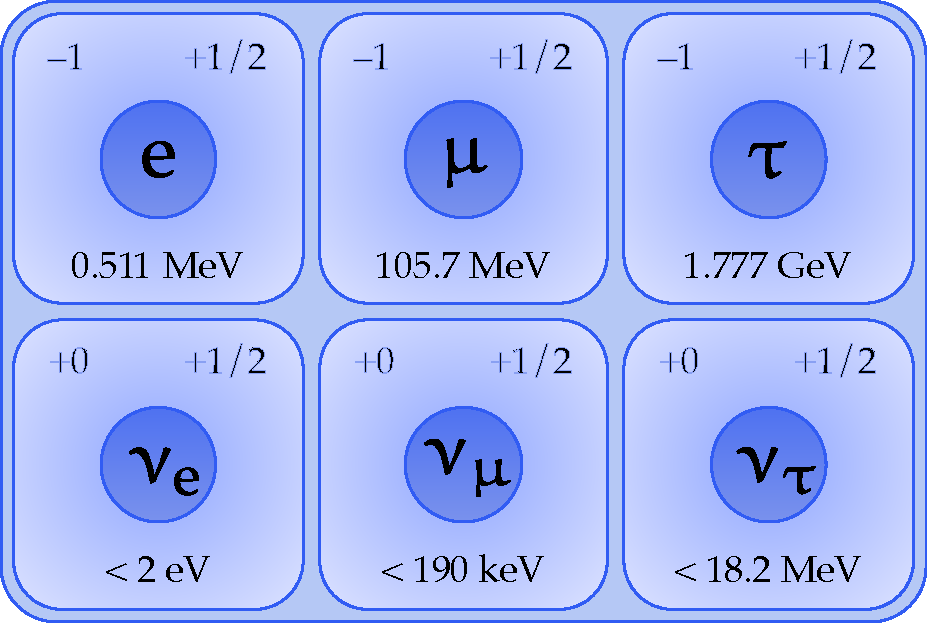
\includegraphics[scale = 0.3]{Leptons.pdf}} \phantom{olaola}
\subfloat[Los 6 leptones en sus 3 generaciones, I, II y III  columna; y sus 2 familias, I y II fila.\label{fig:1b}]{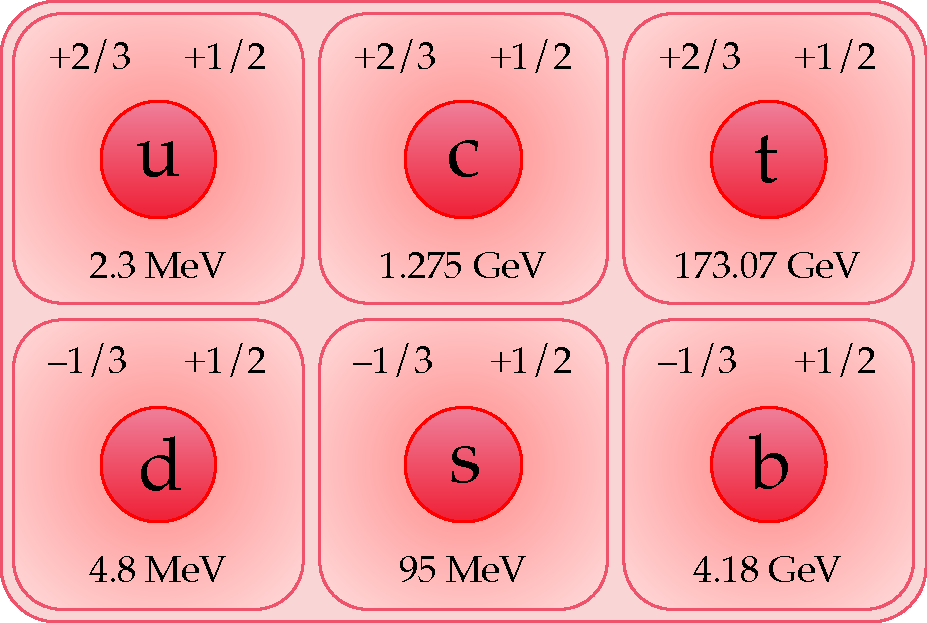
\includegraphics[scale = 0.3]{Quarks.pdf}}\\
%
\subfloat[Bosones \emph{gauge}, portadores de las interacciones.\label{fig:1c}]{\phantom{ola}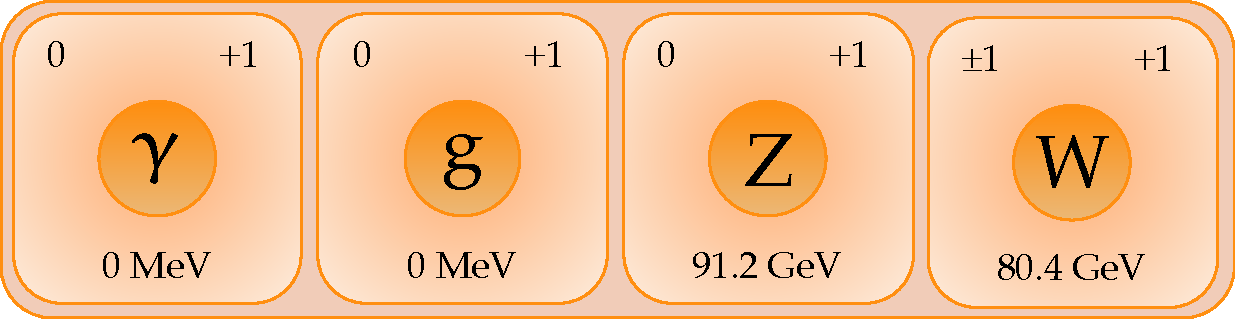
\includegraphics[scale = 0.3]{Bosons.pdf}}\phantom{ola}
\subfloat[Bosón de Higgs.\label{fig:1d}]{\phantom{ola}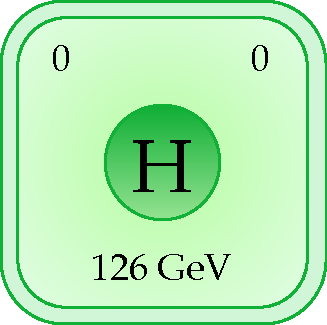
\includegraphics[scale = 0.3]{Higgs.pdf}\phantom{ola}}
\caption{Partículas del \stdmod, los fermiones en las Figuras (a) y (b); y los bosones en las Figuras (c) y (d). En cada cuadro puede verse la carga (arriba izquierda), espín (arriba derecha) y la masa (abajo).} \label{stdmod_particles}
\end{figure}


\color{new}
%%%%%%%%%%%%%%%%%%%%%%%%%%%%%%%%%%%%%%%%%%%%%%%%%%%%%%%%%%%%%%%%%%%%%%%%%%%%%%%%
\subsection{Simetrías discretas en el \stdmod} %%%%%%%%%%%%%%%%%%%%%%%%%%%%%%%%%

La correlación del espín con el espacio--tiempo provoca que existan diferentes estados de una misma partícula. Por ejemplo, se dice que existen fermiones a izquierdas (\emph{left--handed}) o a derechas (\emph{right--handed}), y el operador de paridad, $\OPp$, cambia de una a la opuesta invirtiendo las coordenadas espaciales, es decir, cambiando su helicidad. Aparte del operador $\OPp$, existen otros dos más de transcendental importancia, $\OPc$ y $\OPt$, que se describen a continuación. 



%%%%%%%%%%%%%%%%%%%%%%%%%%%%%%%%%%%%%%%%%%%%%%%%%%%%%%%%%%%%%%%%%%%%%%%%%%%%%%%%
\paragraph{Operador $\bm{\mathsf{\OPt}}$}

La transformación de inversión temporal en física clásica consiste en hacer el cambio $ t \rightarrow - t$; es decir, invertir el sentido del tiempo. Las leyes de la física clásica son  invariantes frente a esta transformación, y en un principio se consideraba que esta era una  simetría verificada de forma exacta por todas las interacciones fundamentales conocidas; de modo que la evidente asimetría temporal en el mundo  macroscópico se atribuía a la muy diferente probabilidad de las configuraciones  macroscópicas iniciales y finales en la evolución de los sistemas. 
%
En la Mecánica  Cuántica hay que encontrar un operador $\OPt$ adecuado para la inversión temporal. Un sistema será simétrico bajo $\OPt$ cuando $[ \OPt, \mathcal{ H}] = 0$ y la función de onda $\OPt \psi$ satisfaga la misma ecuación de  Schrödinger que $\psi$, lo que se traduce en que $\OPt \psi ( t) \neq \psi (- t) = \psi (\bar{ t})$.
%
La transformación correcta de la función de onda bajo el operador $\OPt$ resulta ser $\OPt \psi ( t) = \psi^* (\bar{ t})$, por lo que el operador $\OPt$ es  antiunitario; ello implica que no existen  autoestados del operador $\OPt$, y por lo tanto tampoco números  cuánticos asociados.
%
La interpretación más física de la acción de $\OPt$ es la inversión del movimiento, inviertiendo tanto el momento  linear como el angular.



\paragraph{Operador $\bm{\OPcp}$}

El operador $\OPcp$ se compone de la acción del operador conjugación de carga, $\OPc$, y del operador de paridad, $\OPp$.
%\[ \mathcal{P} |\vec{r}, \vec{p}, \vec{J} \rangle =  |-\vec{r}, -\vec{p}, \vec{J} \rangle  \]
%\[\mathcal{C} | Q, A, L ,S ,C, B, T,  I^3, \vec{p} , \vec{s} \rangle = | -Q, -A, -L ,-S ,-C, -B, -T,  -I^3, \vec{p} , \vec{s} \rangle,\]
%donde 
El operador de paridad invierte las coordenadas espaciales, cambiando de signo la posición y el momento lineal, mientras que mantiene los momentos angulares. Por otra parte, el operador de conjugación de carga mantiene intactas las magnitudes dinámicas, cambiando el signo de los números  cuánticos aditivos: $ Q$, la carga eléctrica; $A$, el número  bariónico; $ L$, el número  leptónico; $I^3$, la tercera componente de  isospín; y $ S, C, B, T$, los números cuánticos de \textit{strange}, \textit{charm}, \textit{beauty} y \textit{truth}, respectivamente.
%
La violación de la  simetría CP implica, en resumidas cuentas, que materia y  antimateria se comportan de forma diferente, y la prueba más evidente de esta violación de  simetría es la preponderancia que existe en el Universo entre materia y  antimateria. En las desintegraciones débiles se violan tanto P como C por separado, pero es mucho más trascendente que  se viole CP, puesto que nos permite definir de manera absoluta qué es materia y qué es  antimateria. Esto ocurre, por ejemplo, en la desintegración  semileptónica del mesón $ K_L^0$, que decae con mayor frecuencia a  positrones que a electrones. 
%
%La violación  CP es realmente desconcertante. 
De acuerdo con la experiencia diaria  macroscópica, no se ve ninguna razón por la que derecha e izquierda deban tener un significado absoluto en la naturaleza. La violación CP no tiene que ver exactamente con el cambio de sentido, sino más bien con la reflexión especular y el cambio de partícula por  antipartícula; es decir, con el cambio de un sistema de referencia  levógiro por otro  dextrógiro.%\footnote{La diferencia clave entre una rotación arbitraria en el espacio y una reflexión espacial es que en esta última un sistema de referencia  dextroxiro pasa a ser  levoxiro, y viceversa.}.



\paragraph{Teorema CPT}

Existe un importante teorema global que permite deducir, entre otras cosas, que la masa y la vida media de las partículas tienen que ser iguales a las de sus  antipartículas. Es el teorema CPT, basado en hipótesis muy generales de la Teoría  Cuántica de Campos y de la Relatividad Especial. Establece que todo  Hamiltoniano que sea  invariante bajo transformaciones de  Lorentz y traslaciones en el espacio--tiempo, que obedezca el principio de  microcausalidad y que tenga un espectro energético con un estado de energía mínimo (el vacío) debe ser  invariante también bajo la acción combinada de los operadores $\OPc$, $\OPp$ y $\OPt$ en cualquier orden. Esto significa que el operador  Hamiltoniano, $\mathcal{ H}$, debe  conmutar con la operación $\OPcp\OPt$; es decir, $[\mathcal{ H},\OPcp\OPt] = 0$.
Aplicar dos veces $\OPcp\OPt$ lleva de nuevo al mismo estado, cuya parte real se corresponde con la masa. Si la partícula es inestable, los autovalores tendrían una parte compleja con información de su anchura y vida media. 
 % y se puede escribir que
%\[ \langle \psi | \mathcal{H} | \psi \rangle = \langle \psi | \mathcal{H} (\mathcal{CPT})^2| \psi \rangle = \langle \psi | \mathcal{CPT} \ \mathcal{H} \ \mathcal{CPT} | \psi \rangle = \langle \overline{\psi} | \mathcal{H} | \overline{\psi} \rangle\]
%donde $\psi$ es el estado correspondiente a una partícula en reposo cuyo  autovalor para el  Hamiltoniano es su masa,  y $\overline{\psi}$ es el estado de su  antipartícula. 
Entonces la  invariancia de $\mathcal{ H}$ frente a $\OPcp\OPt$  predice inmediatamente la igualdad de masa de cada partícula con su  antipartícula.
%Verificar la igualdad de la masa de una partícula y su  antipartícula  es sinónimo de verificar la validez del teorema $\OPcp\OPt$ y de las hipótesis en las que se fundamenta. 
El mejor \textit{test} experimental de la  invariancia $\OPcp\OPt$ en la actualidad lo proporciona la medición de las masas del $ K{}^0$ y del $\overline{ K}{}^0$ (que no son los  autoestados de $\OPcp$): $\left|\frac{ M( K{}^0) -  M(\overline{K}{}^0)}{ M( K{}^0)} \right| \leq 6 \times 10^{-19}$ \cite{pdg2018}.



\color{norm}

\subsection{Lagrangiano} %%%%%%%%%%%%%%%%%%%%%%%%%%%%%%%%%%%%%%%%%%%%%%%%%%%%%%%
\label{sec_yukawa}

Bajo el esquema de partículas de la Figura \ref{stdmod_particles}, se puede construir un lagrangiano, $\mathcal{L}_{\text{\stdmod}}$, que contiene la dinámica de todas las partículas. En él podemos diferenciar la parte relacionada con el bosón de Higgs, $\mathcal{L}_{\text{H}}$, que rompe la simetría $ SU(3)_C \otimes SU(2)_T \otimes U(1)_Y $; y la parte que conserva la simetría, $\mathcal{L}_{\text{FB}}$,
\begin{equation}
\mathcal{L}_{\text{\stdmod}} = \mathcal{L}_{\text{FB}} + \mathcal{L}_{\text{H}}.
\end{equation}
A su vez $\mathcal{L}_{\text{FB}}$ se puede descomponer en las partes correspondientes a quarks (Q), leptones (L) y bosones \emph{gauge} (GB),
\begin{equation}
\mathcal{L}_{\text{FB}} = 3 \mathcal{L}_{\text{Q}} + 3 \mathcal{L}_{\text{L}} + \mathcal{L}_{\text{GB}},	
\end{equation}
y separando las partes cinética ($\mathcal{K}$), que contiene las correspondientes derivadas covariantes que preservan la invariancia \emph{gauge}, y de interacción ($\mathcal{V}$) podemos distinguir
\begin{equation}
\begin{split}
\mathcal{L}_{\text{Q}} &= \mathcal{K}_{\text{Q}} + \mathcal{V}_{\text{Q,EW}} + \mathcal{V}_{\text{Q,S}} \\
\mathcal{L}_{\text{L}} &= \mathcal{K}_{\text{L}} + \mathcal{V}_{\text{L,EW}} .
\end{split}	
\end{equation}

El mecanismo de Higgs, que da masa a las partículas del \stdmod, fue propuesto de modo que las simetrías \emph{gauge} no estuvieran explícitamente rotas. El campo de Higgs rompe la simetría electrodébil de forma espontánea, al tener este un valor de expectación no nulo en el vacío (VEV, \emph{vid.} \S \ref{sec_higgsmecha}). Esta teoría propuesta en la década de los sesenta quedó \color{vero} apoyada \color{norm} en 2012 con el descubrimiento del bosón de Higgs \cite{Aad:2012tfa,Chatrchyan:2012xdj}. Esta parte del lagrangiano la podemos dividir, en consonancia con las anteriores, en
\[\mathcal{L}_{\text{H}} = \mathcal{K}_{\text{H}} + \mathcal{V}_{\text{H,H}} + \mathcal{V}_{\text{H,EW}} + \mathcal{V}_{\text{Y}}\]
siendo $\mathcal{K}$ el término cinemático; $\mathcal{V}_{\text{HH}}$ la interacción consigo mismo y que permite un valor no nulo de $v_0$; $\mathcal{V}_{\text{H,EW}}$ 
que permite dar masa a los bosones $\mathrm{W^{\pm}}$ y $\mathrm{Z^0}$ una vez que se rompe la simetría; y  $\mathcal{V}_{\text{Y}}$ el término de Yukawa que contiene las interacciones fermiónicas que permiten dar masa a los fermiones una vez rota la simetría EW.


\color{new}
\subsection{Mecanismo de Higgs y ruptura espontánea de simetría}
\label{sec_higgsmecha}

Un lagrangiano que contenga tan solo términos de la simetría \emph{gauge} no es suficiente para construir un modelo en el que existan partículas masivas. Si la simetría no se rompe, los bosones carecen de masa; e incluso las masas de los fermiones, bien sean de Dirac o Majorana, también romperían la simetría.
Por otra parte, la simetría $SU(2)_T \otimes U(1)_Y$, que describe la interacción electrodébil, establece una interacción débil que tiene largo alcance, como el electromagnetismo, donde los bosones mediadores tienen masa nula.
Sin embargo, la realidad es bien distinta, puesto que la interacción es de corto alcance 
y está caracterizada por una constante de Fermi,
$G_F$. La simetría \emph{gauge} se encuentra por tanto rota en la naturaleza.


Para explicar este fenómeno se le atribuyó al vacío la
responsabilidad de la ruptura de la simetría, admitiendo la posibilidad de que en él determinados
campos presenten un valor esperado no nulo, lo que vino en llamarse \textit{Electroweak Spontaneous Symmetry Breaking} (EWSSB). Steven Weinberg añadió 4 campos escalares reales de espín cero a la teoría EW $SU(2)_T \otimes U(1)_Y$, dos de ellos con carga ($\phi_1^+$ y $\phi_2^+$) y otros dos neutros ($\phi_3^0$ y $\phi_4^0$), en la forma de un doblete escalar de isospín débil con $I^3 = \sfrac{1}{2}$
\begin{equation}
  \phi(x) = \begin{pmatrix}
    \phi^+(x) \\ \phi^0 (x) 
  \end{pmatrix} = \frac{1}{\sqrt{2}} \begin{pmatrix}
    \phi_1^+(x) + i\phi_2^+(x) \\ \phi_3^0(x) + i\phi_4^0(x) 
  \end{pmatrix}.
\end{equation}
En esta configuración, las 4 partículas escalares tienen hipercarga
débil $Y = +1$. Al campo $\phi_3^0$
se le obliga a tener un valor esperado en el vacío (VEV), $v_0$, muy
elevado: $\phi_3^0(x) = v_0+ H(x)$.
Para ello se postula que el campo $\phi_3^0 (x)$ se encuentra en autoacoplo, siendo la energía potencial de Higgs 
\begin{equation}
V(\phi) = \mu^2 (\phi^{\dagger} \phi) + \lambda (\phi^+ \phi)^2,  \qquad \text{con } \mu^2<0 \text{ y } \lambda >0
\end{equation}
que tiene un estado de mínima energía que se alcanza cuando el campo (sin partículas) toma el valor constante
\[\phi_0 = \langle 0 | \phi | 0 \rangle = \frac{1}{2} \begin{pmatrix}
  0+i0\\ v_0+ i0
\end{pmatrix}\]
siendo $v_0^2 = \frac{-\mu^2}{2 \lambda} = (246.22 \, \mathrm{GeV})^2$. Dicho potencial y su VEV, que se pueden observar en la Figura \ref{fig_higgspot}, dan origen a una partícula de Higgs de masa $M_{\mathrm{H^0}} = \sqrt{2 \lambda v_0^2}$, carga eléctrica neutra e hipercarga $+1$.  

\begin{figure}[H]
\centering

\color{norm}

\begin{tikzpicture}
   \begin{axis}[view={70}{30},
                %colormap={blackwhite}{red!50(0cm)=(1); orange(1cm)=(0)},
                axis lines=middle,axis on top,
                xlabel=$\Re(\phi_0)$,ylabel=$\Im(\phi_0)$,zlabel=$V(\phi_0)$,
                x label style={at={(axis description cs:0.625,0.0)},anchor=west},
                y label style={at={(axis description cs:0.9,0.525)},anchor=west},
                z label style={at={(axis description cs:0.375,0.85)},anchor=west},
                xtick={0.866025},ytick={0.866025},ztick={0},
                xticklabels={$v_0$},
                yticklabels={$v_0$},
                no marks,axis equal,
                xmin=-1.1,xmax=1.1,ymin=-1.1,ymax=1.1,zmin=0,zmax=0.5,
                enlargelimits={upper=0.1}]
     \addplot3[surf, samples=20, samples y=20, domain=0:360, y domain=0:1.3] ({y*sin(x)}, {y*cos(x)}, {-0.6+(y^2 - 0.75)^2});
  \end{axis}
\end{tikzpicture}

\caption{Representación del potencial de Higgs y del VEV.} \label{fig_higgspot}  
\end{figure}



Los bosones \emph{gauge} $\mathrm{W}^{\pm}$ y $Z^0$ adquieren masa a través de la interacción con el bosón de Higgs, mientras que los gluones y fotones no adquieren masa. La simetría $SU(3)_C$ no se ve afectada por el mecanismo de Higgs, lo que explica que los gluones no adquieran masa%, ya que solo interaccionan vía \emph{loops} de quarks
. Sin embargo, los fotones sí interactúan directamente con el campo de Higgs, aunque la conservación de carga eléctrica de quarks y leptones, $Q = I^3 + \frac{Y}{2}$, deja invariante al vacío, y por lo tanto los fotones no adquieren masa. 

Finalmente, los fermiones del \stdmod también se acoplan con el bosón de Higgs y adquieren sus masas, lo que se conoce en la literatura como acoplos de Yukawa. Las nueve constantes de acoplo de los fermiones al campo de Higgs, tal y como aparece en el recuento de la Tabla \ref{tab_stdparams}, son una entrada al \stdmod, que tampoco  explica por qué existen las tres familias de fermiones, idénticas entre ellas y solo distinguibles por su interacción con el campo de Higgs. En el \stdmod los neutrinos son partículas sin masa%; es decir, su helicidad es igual a su quiralidad, por lo que  en él no hay neutrinos a derechas ni tampoco anti--neutrinos a izquierdas
. Sin embargo, experimentalmente, es un hecho conocido que los neutrinos sufren de oscilaciones de sabor, lo que implica que necesariamente han de tener masa\footnote{\label{fn_pmns}El análisis a hacer en esta parte, y no incluído en el \stdmod original, implicaría hacer uso del modelo de \emph{mixing} de Pontecorvo--Maki--Nakagawa--Sakata (PMNS), muy similar al mecanismo de Kobayashi--Maskawa y que explicaría las oscilaciones de neutrinos y les conferiría masa.}.



\color{norm}




%%%%%%%%%%%%%%%%%%%%%%%%%%%%%%%%%%%%%%%%%%%%%%%%%%%%%%%%%%%%%%%%%%%%%%%%%%%%%%%%
%%%%%%%%%%%%%%%%%%%%%%%%%%%%%%%%%%%%%%%%%%%%%%%%%%%%%%%%%%%%%%%%%%%%%%%%%%%%%%%%
\section{Física de sabor en el \stdmod} %%%%%%%%%%%%%%%%%%%%%%%%%%%%%%%%%%%%%%%%
%%%%%%%%%%%%%%%%%%%%%%%%%%%%%%%%%%%%%%%%%%%%%%%%%%%%%%%%%%%%%%%%%%%%%%%%%%%%%%%%
%%%%%%%%%%%%%%%%%%%%%%%%%%%%%%%%%%%%%%%%%%%%%%%%%%%%%%%%%%%%%%%%%%%%%%%%%%%%%%%%

%%%%%%%%%%%%%%%%%%%%%%%%%%%%%%%%%%%%%%%%%%%%%%%%%%%%%%%%%%%%%%%%%%%%%%%%%%%%%%%%
\subsection{El término de Yukawa y la teoría de Kobayashi--Maskawa} %%%%%%%%%%%%



% TODO std mod physics


El término de Yukawa, $\mathcal{V}_{\text{Y}}$, es el único en el \stdmod que distingue entre las familias de fermiones, y es también el responsable de que existan transiciones entre familias de quarks y la violación CP.
En las interacciones electrodébiles los fermiones actúan o bien como singletes, fermiones a derechas tipo \emph{up} y \emph{down}, o como dobletes, fermiones a izquierdas tipo \emph{up} y \emph{down}.

El término de Yukawa se puede separar en la parte correspondiente a quarks y la correspondiente a leptones\footref{fn_pmns}. Centrándose en la parte de quarks,
\begin{equation}
  \begin{pmatrix}
    U\\ D
  \end{pmatrix}_L, U_R, D_R \qquad \text{siendo} \qquad U=\{\mathrm{u,c,t}\},\,\,D=\{\mathrm{d,s,b}\}  
\end{equation}
quedando por tanto el acoplo del Higgs con los campos fermiónicos de quarks,
%\begin{equation}
%\mathcal{V}_{\text{Y,Q}}  = - U_{ij}^d \, \overline{Q_{Li}^I} \, \phi \, d_{Rj}^I  - U_{ij}^{u} \, \overline{Q_{Li}^I} \, \epsilon \phi^*  \, u_{Rj}^I  + h.c. 
%\end{equation}
\begin{equation}
\begin{split}
\mathcal{V}_{\text{Y,Q}}  = & 
- \left[\mathbf{G}^D \left(\overline{U},\!\overline{D} \right)_L \begin{pmatrix}
  \phi^+ \\ \phi^0
\end{pmatrix} D_R + 
\mathbf{G}^U \left(\overline{U},\!\overline{D} \right)_L \begin{pmatrix}
  \overline{\phi}^0 \\ -\phi^-
\end{pmatrix} U_R \right] \\ & +
%
%
\left[\mathbf{G}^{D*} \overline{D}_R\left(\phi^-,\!\overline{\phi}^0 \right) \begin{pmatrix}
  U \\ D
\end{pmatrix}_L + 
\mathbf{G}^{U*} \overline{U}_R \left(\phi^0,\!-\phi^+ \right) \begin{pmatrix}
  U \\ D
\end{pmatrix}_L \right]
\end{split}
\end{equation}
siendo $\mathbf{G}^{U,D}$ matrices $3\times3$, en general complejas. Cuando se produce la EWSB, el campo de Higgs ($\phi$) adquiere su VEV en el vacío y la ecuación previa confiere masas a los quarks. 

Para obtener los estados \emph{físicos} de los quarks (autoestados de masa), las matrices $\mathbf{G}^{U,D}$ deben diagonalizarse (en una matriz diagonal $\mathbf{M}$) respecto a matrices unitarias, tales que $\mathbf{M}^{\{U,D\}}=\mathbf{V}_L^{\{U,D\}} \mathbf{G}^{\{UD\}} {\mathbf{V}_R^{\{U,D\}}}^{\dagger}$.
%
Como consecuencia, las corrientes cargadas acoplan al bosón $\mathrm{W^{\pm}}$ interaccionando con los quarks con términos de la forma
\begin{equation}
	-\frac{G_F}{\sqrt{2}} \left( W_{\mu}^+ \overline{U}_L \gamma^{\mu}  \vckm D_L + W_{\mu}^- \overline{D}_L \gamma^{\mu}  \vckm^+ U_L \right)
\end{equation}
donde $G_F$ es la constante de Fermi (la constante de acoplo débil), $\gamma^{\mu}$ las matrices de Dirac, y $\vckm= \mathbf{V}_L^U {\mathbf{V}_L^D}^{\dagger}$ es la matriz de mezcla de Cabibbo--Kobayashi--Maskawa \cite{pdg2018}, dada por \color{new}
\begin{align}
  \vckm  &= \begin{pmatrix}
	V_{ud} & V_{us} & V_{ub} \\
	V_{cd} & V_{cs} & V_{cb} \\
	V_{td} & V_{ts} & V_{tb} \\
\end{pmatrix} \\ & \approx \begin{pmatrix}
0.97427 \pm 0.00015 & 0.22534 \pm 0.00065 & 0.00351^{+0.00015}_{-0.00014} \\
0.22520 \pm 0.00065 & 0.97344 \pm 0.00016 & 0.0412^{+0.0011}_{-0.0005} \\
0.00867^{+0.00029}_{-0.00031} & 0.0404^{+0.0011}_{-0.0005} & 0.999146^{+0.000021}_{-0.000046}
\end{pmatrix}. \nonumber
\end{align}

La matriz es no diagonal, y su estructura permite transiciones entre las diferentes generaciones de quarks, dando lugar a procesos con intercambio de sabor pero no de carga. Estos procesos denominados de \textit{Flavour Changing Neutral Currents} (FCNC), que es donde precisamente se ven involucradas las fases de la matriz y donde emana la violación CP. Es también gracias a la no diagonalidad de la matriz que se pueden producir las oscilaciones partícula--antipartícula de mesones neutros, que se detallarán en \S \ref{sec_neutralmesons}.



\color{vero}
La matriz $\vckm$ admite diferentes parametrizaciones, entre ellas la parametrización de Wolfenstein resulta particularmente útil, pues permite, dado que todos sus parámetros son de orden 1, desarrollar la matriz en potencias de $\lambda$. Sus parámetros, definidos en función de los elementos de $\vckm$, son,
\[ \lambda = \frac{|V_{\text{us}}|}{\sqrt{|V_{\text{ud}}|^2+|V_{\text{us}}|^2}}, \quad A \lambda^2 = \lambda \left|\frac{V_{\text{cb}}}{V_{\text{us}}}\right|\quad \text{y} \quad A \lambda^3 (\rho + i \eta ) V_{\text{ub}}^* . \] \color{norm}
de modo que resulta
\begin{equation}
\begin{split}
\vckm   & = \begin{pmatrix} 1-\lambda^2/2 & \lambda & A\lambda^3(\rho-i\eta) \\
 -\lambda & 1-\lambda^2/2 & A\lambda^2 \\
 A\lambda^3(1-\rho-i\eta) & -A\lambda^2 & 1  \end{pmatrix} + \mathcal{O}(\lambda ^4 )= \\ & =
 \left(\begin{array}{lll}
	\phantom{-} |V_{ud}| & \phantom{-}|V_{us}| & \phantom{-}|V_{ub}|e^{-i\gamma} \\
	-|V_{cd}| & \phantom{-}|V_{cs}| & \phantom{-}|V_{cb}| \\
	  \phantom{-}|V_{td}|e^{-i\beta} &-|V_{ts}|e^{i\beta_s} & \phantom{-}|V_{tb}| \\
\end{array}\right) + \mathcal{O}(\lambda ^5 ).
\end{split}	
\end{equation}
\color{vero}


%

No son medibles cada una de las fases individuales de los $2\times3$ quarks, ni tampoco la fase global de $\vckm$. Si se considera que $\vckm$ es $N \times N$ generaciones de quarks, entonces por ser unitaria tiene $N^2$ parámetros reales. 
De estos solo son medibles $(N-1)^2 = N^2 - (2N-1)$, puesto que se puede absorber una fase en cada campo de quarks, y la fase global \textit{no} es observable. Ahora bien, si $\vckm$ fuese real, solo tendría $\frac{1}{2} N(N -1)$ parámetros reales, quedando como parámetros complejos medibles $\frac{1}{2}(N-1)(N-2)$ fases. \color{norm}
%
La matriz $\vckm$, de $N=3$ generaciones, se parametriza con 3 parámetros reales y una fase compleja, y es precisamente esta última la que es fuente de violación CP en el \stdmod (\emph{vid.} Apéndice \ref{ap_cpvio}).

\begin{figure}[H]
\centering
\subfloat[Triángulo unitario que se forma para el mesón $\text{B}{}^0$.\label{fig_ckmd}]{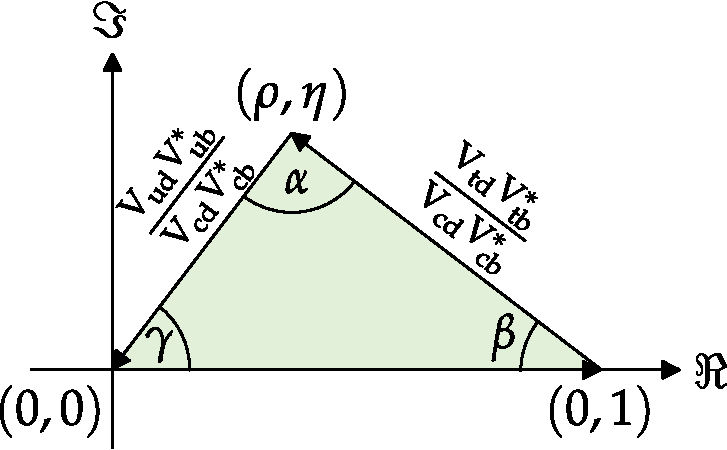
\includegraphics[height=0.25\textwidth]{Triangle2.pdf}} \hfill
\subfloat[Triángulo unitario que se forma para el mesón $\text{B}{}_s^0$.\label{fig_ckmb}]{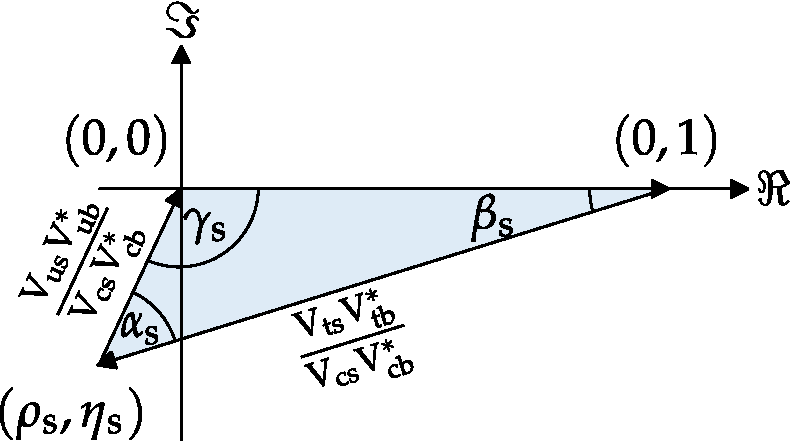
\includegraphics[height=0.25\textwidth]{Triangle1.pdf}} \hfill
%
\caption{Dos de los triángulos que se pueden construir con los elementos de $\vckm$ y la condición de unitariedad. Los triángulos no se encuentran dibujados a escala.}	
\end{figure}


Por la condición de unitariedad se pueden construir diferentes triángulos con la matriz $\vckm$, que son motivo de profundos estudios de precisión del modelo de Kobayashi--Maskawa, entre ellos verificar la unitariedad de esta matriz. Uno de ellos, aunque casi degenerado en rectas, es el reflejado en la Figura \ref{fig_ckmb},
\begin{equation}
 V_{\mathrm{us}} V_{\mathrm{ub}}^* + V_{\mathrm{cs}} V_{\mathrm{cb}}^* + V_{\mathrm{ts}} V_{\mathrm{tb}}^* = 0 
\end{equation}
siendo el menor de los ángulos de este triángulo,
\begin{equation}
	\beta_{\mathrm{s}} =  \text{arg} \left( - \frac{V_{\mathrm{ts}} V_{\mathrm{tb}}^*}{V_{\mathrm{cs}} V_{\mathrm{cb}}^*}   \right)  \label{eq_bs_ckm}
\end{equation}
\color{vero} Asumiendo el \stdmod, y haciendo un ajuste global combinando datos experimentales \cite{ckmfitter1}, se predice el valor  , %cuyo valor se pretende medir por primera vez en esta tesis, y encontrarlo no compatible con cero.
\begin{equation}
	\varphi_{\text{s}}^{\text{SM}} = -2 \beta_{\text{s}} = -36.9\,{}_{-0.8}^{+1.0} \, \text{mrad}. \label{eq_smpredicphis}
\end{equation} \color{norm}
\color{dieg} Cualquier desviación en el valor de $\varphi_{\text{s}}$ (\emph{vid.} \S\ref{sec_phis}), grande o pequeña, es una evidencia de física \bstdmod, haciendo que  sea un excelente observable para estas búsquedas. \color{norm}
%TODO ajuste emph

\subsection{Sistemas de mesones neutros} %%%%%%%%%%%%%%%%%%%%%%%%%%%%%%%%%%%%%%%
\label{sec_neutralmesons}

El número cuántico de sabor es conservado por dos de las interacciones del \stdmod: la electromagnética y la interacción nuclear fuerte. Sin embargo, la interacción débil no conserva el sabor, $\Delta F \neq 0$. Sin pérdida de generalidad, se hará referencia al mesón $\Bs$ como un mesón neutro genérico, puesto que es el \color{vero}estudiado \color{norm} en este trabajo. 

El mesón $\Bs[\mathrm{s\bar b}]$ es un mesón neutro y que tiene por antipartícula al mesón $\Bbs[\mathrm{\bar s b}]$, que es su conjugado en el número cuántico de sabor y también neutro. Ambos pueden convertirse en su antipartícula mediante un proceso denominado oscilaciones mesón--antimesón, propiedad que comparten con todos los mesones neutros pesados. Las oscilaciones de mesones  son posibles en el \stdmod mediante diagramas como los de las Figura \ref{fig_mixing}, y juegan un papel muy importante en la física de sabor, puesto que son muy sensibles a la existencia de nuevas partículas. 

\begin{figure}[H]
\centering
\subfloat{\includegraphics[width=0.48\textwidth,page=3]{feymans.pdf}} \hfill
\subfloat{\includegraphics[width=0.48\textwidth,page=4]{feymans.pdf}} \hfill
\caption{Diagramas de Feynman para la mezcla $\Bs - \Bbs$.} \label{fig_mixing}
\end{figure}


La existencia de la interacción nuclear débil es la que provoca que estos mesones decaigan a otras partículas; sin ella, ambos mesones, $\Bs$ y $\Bbs$, serían un par partícula--antipartícula estable con masa $m_0$, y común a ambos. Así pues, puede decirse que $|\Bs\rangle$ y $|\Bbs\rangle$ son autoestados de las interacciones nuclear fuerte y electromagnética, siendo por tanto $\langle \Bs | \Bbs \rangle = 0$. Sin embargo, una vez se considere el hamiltoniano débil, $\HW$, este provocará que ambos mesones oscilen y decaigan a otros estados \cite{lavoura}.

Se puede escribir el hamiltoniano del sistema en dos partes diferenciadas,
\[\mathcal{H} = \mathcal{H}_0 + \HW ,\]
una que cumple $\Delta F =0$, el operador $\mathcal{H}_0$; y la parte débil, que tratamos como una perturbación, el operador $\HW$.



\subsubsection{Matriz de masa--desintegración}

Como causa del \emph{mixing} de sabor, los mesones neutros están sujetos a oscilaciones partícula--antipartícula, a través de transiciones débiles que cambian el sabor en 2 unidades ($\Delta F = 2$) o bien mediante un estado intermedio (con $\Delta F = 1$). En este caso, la corriente neutra de cambio de sabor (FCNC), que cambia el sabor en 2 unidades, es la responsable de las oscilaciones $\Bs - \Bbs$ ilustradas en los diagramas de Feynman de las Figura \ref{fig_mixing}, y denominados por su topología diagramas de caja. Como resultado de la mezcla de sabor, el estado inicial después de la creación del mesón es una superposición de los estados con $\Bs $ y $\Bbs$,
\[|\psi(t)\rangle = a(t) |\Bs\rangle + b(t) |\Bbs\rangle.\]
%
En la aproximación de Wigner--Weisskopf, que omite las correcciones a la tasa de desintegración exponencial para tiempos muy bajos
%\footnote{El tiempo característico de la interacción fuerte es --.., y nosotros no s interesaremos por estado con $t\gg\tau_S$.} 
o muy altos, el hamiltoniano efectivo del sistema se puede escribir como 
\[\mathcal{H}_{\text{eff}} = \begin{pmatrix}
	M_{11} & M_{12} \\ M_{12}^* & M_{22}
\end{pmatrix} - \frac{i}{2} \begin{pmatrix}
	\Gamma_{11} & \Gamma_{12} \\ \Gamma_{12}^* & \Gamma_{22} 
\end{pmatrix} = \mathbf{M} - \frac{i}{2} \bm{\Gamma} \]
%
\noindent y que no es hermítico\footnote{Sin embargo, tanto $\mathbf{M}$ como $\bm{\Gamma}$ sí son matrices hermíticas ($\mathbf{M} = \mathbf{M}^{\dagger}$ y $\bm{\Gamma} = \bm{\Gamma}^{\dagger}$), verificando además que $\bm{M}=\frac{1}{2} (\mathcal{H}_{\text{eff}} + \mathcal{H}_{\text{eff}}^{\dagger})$ y $\bm{\Gamma} = i(\mathcal{H}_{\text{eff}}-\mathcal{H}_{\text{eff}}^{\dagger})$.}, en cuyo caso los mesones no decaerían y simplemente oscilarían. Este hamiltoniano ha de verificar la ecuación de Schrödinger
\[i \frac{d}{dt} \begin{pmatrix}
	a(t)  \\ b(t)
\end{pmatrix} = \mathcal{H}_{\text{eff}} \begin{pmatrix}
	a(t)   \\ b(t)  
\end{pmatrix}.\]
%
Expandiendo a segundo orden en teoría de perturbaciones \cite{lavoura}, se encuentra que los elementos de las matrices de masa y desintegración son, 
\[M_{ij} = m_0 \delta_{ij} + \langle i | \HW^{\Delta F = 2} | j\rangle  + \sum_k \mathbb{P} \frac{\langle i | \HW^{\Delta F = 1} | k\rangle \langle k | \HW^{\Delta F = 1} | j \rangle }{m_0 - E_k}\]
\[\Gamma_{ij} = 2 \pi \sum_k \delta (m_0 - E_k) \langle i | \HW^{\Delta F = 1} | k\rangle \langle k | \HW^{\Delta F = 1} | j \rangle .\]

En virtud de la invariancia CPT, $M \equiv M_{11} = M_{22}$ y $\Gamma \equiv \Gamma_{11}=\Gamma_{22}$. Los términos no diagonales son responsables del fenómeno de mezcla $\Bs - \Bbs$, que se produce con una frecuencia $\omega$ de oscilación de CKM, donde, para este caso $\Bs$, se involucra al elemento $ V{}_{\text{tb}}^* V{}_{\text{ts}}$. La parte dispersiva $M_{12}$ se corresponde con partículas virtuales de transiciones $\Delta F = 2$ y que están dominadas por partículas muy pesadas en el \stdmod, como el quark \textit{top}. La parte absortiva, $\Gamma_{12}$, se corresponde con transiciones de capa debidas a los modos desintegración que son comunes tanto a mesón como a anti--mesón, $\Delta F = 1$. Ninguno de estos últimos es autoestado de $\mathcal{H}$, puesto que no lo son de $\mathcal{H}_W$ (aunque sí de $\mathcal{H}_0$), por lo que se necesita construir una nueva base. Diagonalizando el hamiltoniano respecto de una base ${\Bs}_{H,L}$, pesado y ligero respectivamente, aparecen estos dos autoestados que no oscilan, simplemente decaen. A cada uno de ellos les corresponde una masa $M_{H,L}$ y una anchura $\Gamma_{H,L}$. Los autovalores son
%
\[\mu_{H,L} = M - i\frac{\Gamma}{2} \pm Q = M - i\frac{\Gamma}{2} \pm \sqrt{\left(M_{12}-i\frac{\Gamma_{12}}{2}\right) \left(M_{12}^*-i\frac{\Gamma_{12}^*}{2}\right)}\]
de donde se sigue que 
\[\Delta m = M_H - M_L =2 \Re (Q) \qquad \Delta \Gamma = \Gamma_L - \Gamma_H = 4 \Im (Q).\]
% $m = \frac{m_H + m_L }{2}$ y $\Gamma = \frac{\Gamma_H + \Gamma_L}{2}$
 
Los autoestados son mezclas de los estados de sabor, con coeficientes complejos, $p$ y $q$, que satisfacen $p^*p + q^*q = 1$,
%
\[| {\Bs}_{H,L} \rangle = p |\Bs \rangle \pm q | \Bbs \rangle \]
%
siendo 
\begin{equation}
\frac{q}{p}  = \pm \sqrt{\frac {M_{12}^*-i\frac{\Gamma_{12}^*}{2}} {M_{12}-i\frac{\Gamma_{12}}{2}} }	.\label{eq_qp_cocient}
\end{equation}



\subsubsection{Evolución temporal} %%%%%%%%%%%%%%%%%%%%%%%%%%%%%%%%%%%%%%%%%%%%%%%%
\label{sec_evotempB}

La evolución temporal de los dos autoestados viene dada por los autovalores,
\[|{\Bs}_{H,L} (t) \rangle  = e^{-i \mu_{H,L}t } |{\Bs}_{H,L} (0)\rangle = e^{-i (m_{H,L} - \frac{1}{2} \Gamma_{H,L})t} |{\Bs}_{H,L} (0)\rangle. \]
Por su parte, la evolución temporal de los estados de sabor, $\Bs$ y $\Bbs$, viene dada por las dos siguientes ecuaciones
\begin{equation}
\begin{split}
|\Bs\rangle  = g_+(t) |\Bs\rangle  + \frac{q}{p} g_-(t) |\Bbs\rangle\\
|\Bbs\rangle = g_+(t) |\Bbs\rangle + \frac{p}{q} g_-(t) |\Bs \rangle
\end{split}	
\end{equation}
%
con la dependencia temporal expresada mediante las funciones
\begin{equation}
\begin{split}
g_{\pm}(t) &=  \frac{1}{2} \left( e^{-iM_Lt} e^{-\frac{\Gamma_L}{2} t} \pm e^{-iM_Ht} e^{-\frac{\Gamma_H}{2} t} \right) \\
& = \frac{1}{2} e^{-im_{\Bs}t} e^{-\frac{\Gamma}{2}t} \left( e^{i\frac{\Delta m}{2}t} e^{-\frac{\Delta \Gamma}{4}t}  \pm e^{-i\frac{\Delta m}{2}t} e^{\frac{\Delta \Gamma}{4}t} \right).	
\end{split} \label{eq_gedete}
\end{equation}
%
%
%
%\[|g_{\pm}(t)|^2 = \frac{e^{-\Gamma t}}{2} \left[ \cosh \frac{\Delta \Gamma t}{2} \pm \cos \Delta m t \right]\]
%\[g_+^* g_-(t) = -\frac{e^{-\Gamma t}}{2} \left[ \sinh \frac{\Delta \Gamma t}{2} \pm i\sin \Delta m t \right] \]
%
%

\begin{figure}[H]
\centering
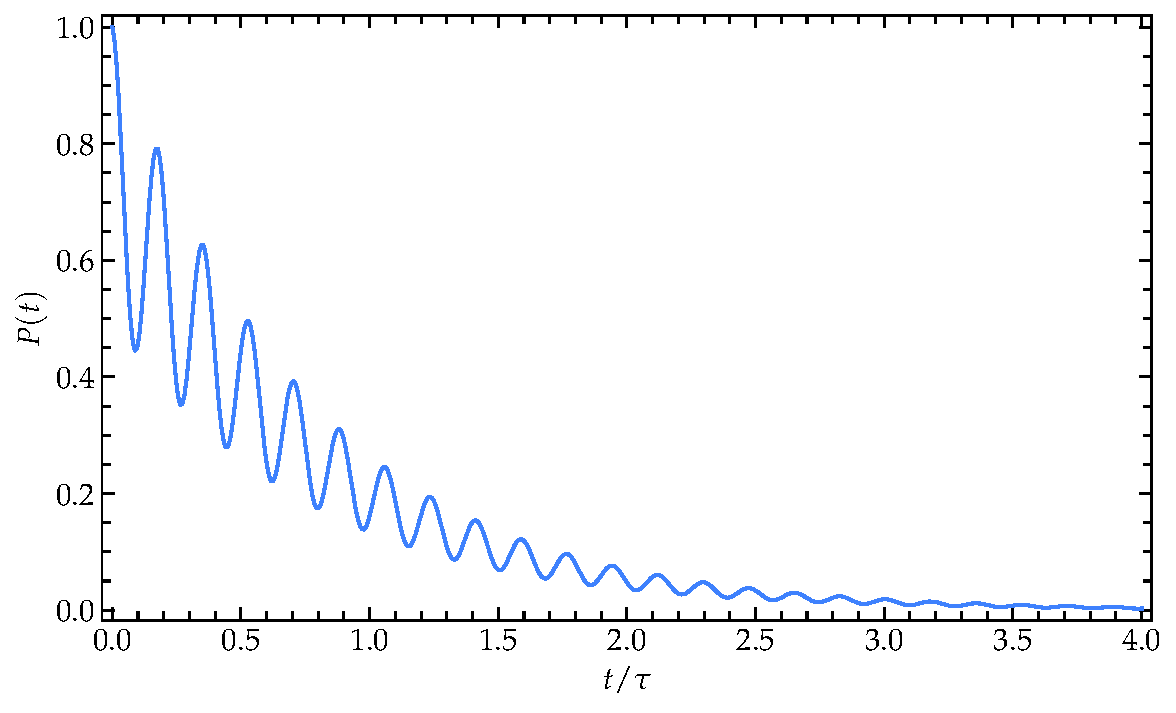
\includegraphics[width=0.48\textwidth]{plots/gpm_total}	 \hfill
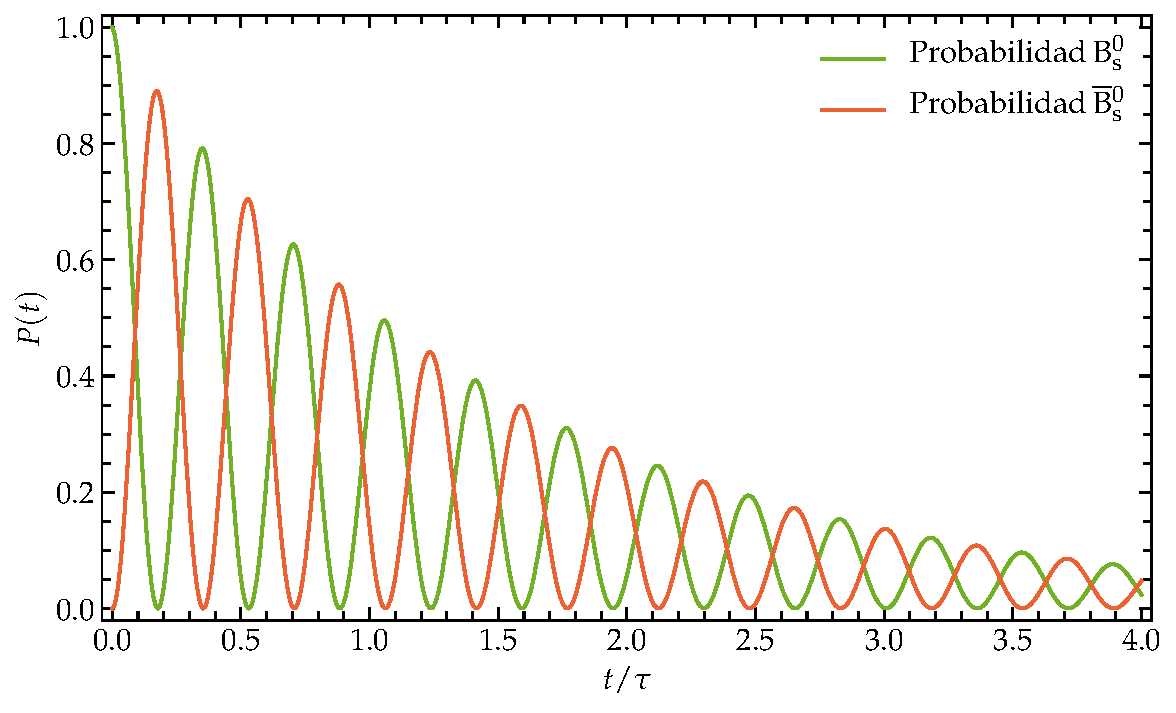
\includegraphics[width=0.48\textwidth]{plots/gpm_bbbar}	 \hfill
\caption{Probabilidad de observar un mesón $\Bs \text{ o } \Bbs$ --- conjuntamente  (izquierda) y separadamente (derecha) --- a tiempo $t$ \color{vero} y para un suceso inicial $\Bs$. \color{norm} }
\end{figure}

Entonces, para un determinado estado final $|f\rangle$ (y su conjugado), existen las cuatro siguientes posibles amplitudes
\begin{equation}
\begin{split}
\mathcal{A}_f = \langle f | \HW | \Bs \rangle \qquad \qquad\mathcal{A}_{\bar f} = \langle \bar f | \HW | \Bs \rangle \\
\overline{\mathcal{A}_f} = \langle f | \HW | \Bbs \rangle \qquad \qquad \overline{\mathcal{A}_{\bar f}} = \langle \bar f | \HW | \Bbs \rangle
\end{split}
\end{equation}
%
\color{vero} y donde se puede definir la cantidad compleja que gobierna las simetrías CP, 
%
\begin{equation}
\lambda_f = \frac{q}{p} \frac{\overline{\mathcal{A}_f}}{\mathcal{A}_f}.
\end{equation}
\color{norm}






\subsection{Violación CP} %%%%%%%%%%%%%%%%%%%%%%%%%%%%%%%%%%%%%%%%%%%%%%%%%%%%%%


\color{vero} La parte teórica \color{norm}  precisa de la existencia de una fase (\emph{vid.} Apéndice \ref{ap_cpvio}), lo que implica en el terreno experimental que esta fase cuántica compleja aparezca y sea medida en procesos de interferencia. Estos procesos han de ser de amplitudes de tamaño similar y que interfieran entre ellas. Si se consideran las secciones eficaces para los procesos $\text{M} \rightarrow f $ y $\overline{\text{M}} \rightarrow \bar f $, se da la siguiente proporcionalidad:
\[\Gamma (\text{M} \rightarrow f )  \sim e^{-\Gamma t} \, |\mathcal{A}_f|^2 \, \left| \frac{p}{q} \right|^2 \qquad	
\overline{\Gamma} (\overline{\text{M}} \rightarrow \bar f )  \sim e^{-\Gamma t} \,  |\overline{\mathcal{A}}_{\bar f}|^2 \, \left| \frac{p}{q} \right|^2.\]
A la vista de las expresiones, para ver cómo la interferencia entre amplitudes se ve reflejada en los módulos cuadrados y dónde podrían estar incluidas las fases que violarían la simetría CP, es útil escribir las amplitudes de la siguiente forma \color{vero}
\begin{equation}
\begin{split}
\mathcal{A}_f & = A_1 e^{i(\delta_1+\varphi_1)}	 + A_2 e^{i(\delta_2+\varphi_2)}	\\
\overline{\mathcal{A}}_{\overline{f}} & = A_1e^{i(\delta_1-\varphi_1)}	 + A_2e^{i(\delta_2-\varphi_2)}	
\end{split}
\end{equation} \color{norm}
donde la cantidad de violación CP vendrá dada por las llamadas fases de violación CP, $\varphi$, que emanan de los términos del lagrangiano que violan CP (es decir, que cambian de signo al aplicarle $\OPcp$). En el SM esto solo puede suceder mediante la interacción débil  y por lo tanto estas fases suelen denominarse fases débiles.  Las fases que conservan CP, $\delta$, provienen de términos del lagrangiano que son invariantes bajo $\OPcp$, y en el SM están típicamente relacionadas con la interacción fuerte, y por ello se denominan fases fuertes o hadrónicas.
Además, para el caso de mesones neutros, como el $\Bs$, es útil definir
\begin{equation}
	M_{12} = |M_{12}|e^{i\varphi_M}, \qquad \Gamma_{12} = |\Gamma_{12}|e^{i\varphi_{\Gamma}}
\end{equation}
%
En la literatura \cite{lavoura}, suelen distinguirse 3 tipos de violación CP ligadas a asimetrías entre amplitudes, $\mathscr{A}$, que se desglosan a continuación.



\subsubsection{Violación CP directa: CPV en la desintegración} %%%%%%%%%%%%%%%%%
\label{sec_CPVdesint}

Cuando las amplitudes de los procesos $A_f$ y $\overline{A}_{\bar f}$ (el proceso conjugado)  son distintas, entonces se tiene violación CP dado que \cite{pdg2018}
\begin{equation*}
\left| \frac{A_f}{\overline{A}_{\bar f}} \right| \neq 1 \qquad \Rightarrow \qquad \mathscr{A} _D = \frac{\overline{\Gamma}-\Gamma}{\overline{\Gamma}+\Gamma}=\frac{ \left| \sfrac{\overline{\mathcal{A}}_{\overline{f}}}{\mathcal{A}_f} \right|^2 -1 }{\left| \sfrac{\overline{\mathcal{A}}_{\overline{f}}}{\mathcal{A}_f} \right|^2 +1}.
\end{equation*}
%
Esta diferencia puede medirse en un proceso de interferencia y ser enorme puesto que 
\begin{equation}
\mathscr{A}_D \propto |A_f|^2 - |\overline{A}_{\overline{f}}|^2 = -4A_1A_2 \sin(\delta_1 - \delta_2) \sin (\varphi_1 - \varphi_2).	\label{eqinferf1}
\end{equation}
\color{vero} Esta \color{norm} es la única fuente de violación CP en sistemas de mesones cargados (puesto que estos no se ven afectados por la mezcla, $\Delta F = 1$).



\subsubsection{Violación CP indirecta: CPV (y TV) en la mezcla} %%%%%%%%%%%%%%%%
\label{sec_CPVmixing}

\color{vero} Se define la violación CP en la mezcla mediante \cite{pdg2018}\color{rem}
\begin{equation}
 \left| \frac{q}{p} \right| \neq 1	\qquad \Rightarrow \qquad \mathscr{A}_M = \frac{\sfrac{d\overline{\Gamma}}{dt}-\sfrac{d\Gamma}{dt}}{\sfrac{d\overline{\Gamma}}{dt}+\sfrac{d\Gamma}{dt}}  =  \frac{1- \left| \sfrac{q}{p} \right|^4}{1+ \left| \sfrac{q}{p} \right|^4},
\end{equation} 
un tipo de violación CP que se ha visto y medido en desintegraciones semileptónicas. Nótese que esta asimetría de tasas de desintegración dependientes del tiempo es, de hecho, no dependiente del tiempo.  \color{norm}

Si se manifiesta esta violación CP, vendría a indicar que en los procesos con $\Delta F = 2$ la mezcla que se produce en las Figuras \ref{fig_mix_a} y \ref{fig_mix_b} es distinta. Un proceso de violación CP en este caso requeriría de contribuciones en \color{vero} la mezcla \color{norm} que son similares en tamaño. Bajo la aproximación $M_{12} \gg \Gamma_{12}$ (válida para el $\Bs$), esta asimetría en desintegraciones de mesones neutros es
\begin{equation}
\mathscr{A}_M \propto \left| \frac{\Gamma_{12}}{M_{12}} \right| \sin (\varphi_M - \varphi_{\Gamma}),	
\end{equation}
aunque se trata de un factor pequeño y difícil de calcular, puesto que involucra \emph{long--distance physics}.



\subsubsection{Violación CP en la interferencia} %%%%%%%%%%%%%%%%%%%%%%%%%%%%%%%
\label{sec_cpvinter}

\begin{wrapfigure}{r}{0.45\textwidth}
\centering
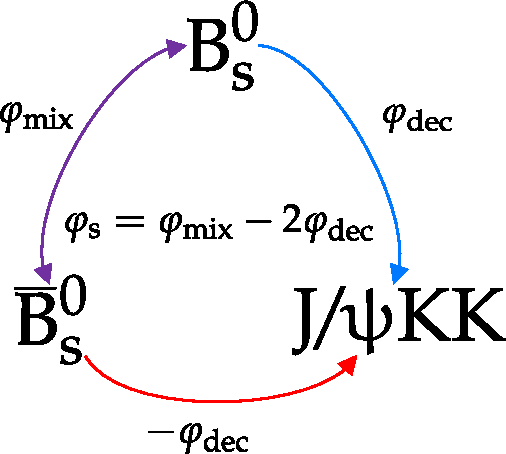
\includegraphics[width=0.3\textwidth]{PhisScheme.pdf}
\caption{Interferencia entre la desintegración directa y la desintegración después de la mezcla.}	\label{fig_oscillatenoscillate}
\end{wrapfigure}
Medir violación CP a través de asimetrías directas (\S \ref{sec_CPVdesint}) o en el \emph{mixing} (\S \ref{sec_CPVmixing}) no es la única forma de acceder a las fases de la matriz $\vckm$. Se puede también medir procesos de interferencia más sutiles donde no haya tanto protagonismo de las fases fuertes\footnote{\color{vero}En la Ecuación (\ref{eqinferf1}), se observa el seno de la diferencia de fases fuertes, que puede ser pequeño en algunos casos; y en dichos casos 'suprime' la posibilidad de observar los fenómenos de interferencia. \color{norm}}.
%
La interferencia puede producirse entre la desintegración del mesón y su oscilación partícula--antipartícula, en el estado entrelazado que se produce antes de la desintegración.
%
La teoría EW es capaz, por sí misma, de convertir espontáneamente un mesón neutro en su antipartícula a través, principalmente, del quark \textit{top}, aunque también de \emph{up} y \emph{charm}, como se observa en las Figuras \ref{fig_mix_a} y \ref{fig_mix_b}: se van intercambiando $\Bs$ y $\Bbs$ con una cierta frecuencia. Si ambos mesones tienen el mismo estado final, $f = \overline{f}$,  entonces estos podrán decaer al estado final habiendo o no oscilado previamente (\emph{vid.} Figura \ref{fig_oscillatenoscillate}).
%
Es posible observar violación CP incluso en ausencia de violación CP directa e indirecta, $|\lambda_f| = 1$. En este caso, $\lambda_f$ es una fase pura, típicamente \cite{pdg2018}, 
\begin{equation}
	\Im(\lambda_f) \neq 0  \,\, \Rightarrow \,\, \mathscr{A}_{\lambda} = \frac{
	\sfrac{d{\Gamma}(\overline{M}\rightarrow f )}{dt}-\sfrac{d\Gamma({M}\rightarrow f )}{dt}}{
	\sfrac{d{\Gamma(\overline{M}\rightarrow f )}}{dt}+\sfrac{d\Gamma({M}\rightarrow f )}{dt}} \propto \Im (\lambda_f) \sin (\Delta m \, t). \label{eq_alanda}
\end{equation}
%
De este modo, la fase medida aquí sería una fase débil, sin influencia de fases hadrónicas.



%%%%%%%%%%%%%%%%%%%%%%%%%%%%%%%%%%%%%%%%%%%%%%%%%%%%%%%%%%%%%%%%%%%%%%%%%%%%%%%%
%%%%%%%%%%%%%%%%%%%%%%%%%%%%%%%%%%%%%%%%%%%%%%%%%%%%%%%%%%%%%%%%%%%%%%%%%%%%%%%%
%%%%%%%%%%%%%%%%%%%%%%%%%%%%%%%%%%%%%%%%%%%%%%%%%%%%%%%%%%%%%%%%%%%%%%%%%%%%%%%%

\bigskip

\begin{center}
	$***$
\end{center}

\medskip

%%%%%%%%%%%%%%%%%%%%%%%%%%%%%%%%%%%%%%%%%%%%%%%%%%%%%%%%%%%%%%%%%%%%%%%%%%%%%%%%
%%%%%%%%%%%%%%%%%%%%%%%%%%%%%%%%%%%%%%%%%%%%%%%%%%%%%%%%%%%%%%%%%%%%%%%%%%%%%%%%
%%%%%%%%%%%%%%%%%%%%%%%%%%%%%%%%%%%%%%%%%%%%%%%%%%%%%%%%%%%%%%%%%%%%%%%%%%%%%%%%

\begin{subappendices}

%\titleformat{\section} 
%  {\normalfont}{\spacedlowsmallcaps\appendixname\ %
%  {\spacedallcaps\thesection}}%
%  {1em}{\spacedallcaps}

%%%%%%%%%%%%%%%%%%%%%%%%%%%%%%%%%%%%%%%%%%%%%%%%%%%%%%%%%%%%%%%%%%%%%%%%%%%%%%%%



%%%%%%%%%%%%%%%%%%%%%%%%%%%%%%%%%%%%%%%%%%%%%%%%%%%%%%%%%%%%%%%%%%%%%%%%%%%%%%%%
\section{Fases de CKM y violación CP}  %%%%%%%%%%%%%%%%%%%%%%%%%%%%%%%%%%%%%%%%%
\label{ap_cpvio}

La fase compleja de la matriz CKM es la única fuente de violación CP que se contempla en el sector electrodébil\footnote{Siendo precisos, puede existir violación CP que provenga de interacciones fuertes, mediante el parámetro de violación CP de QCD (\emph{vid.} Tabla \ref{tab_stdparams}). Sin embargo, este parámetro es muy pequeño e irrelevante en el caso de desintegraciones hadrónicas.} de quarks en el \stdmod. Este mecanismo no permite explicar la gran asimetría materia--antimateria que se observa en el Universo actual, por lo tanto deben existir otros procesos adicionales que dieron lugar a esta composición.

Para ver por qué las fases de $\vckm$ tienen la capacidad de generar violación CP, vamos a suponer una colisión a 2 cuerpos entre quarks libres, que denominaremos genéricamente $a\,b \rightarrow c\,d$.
\begin{figure}[H]
\centering
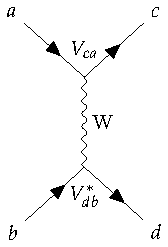
\includegraphics[width = 0.25\textwidth, page =1]{feymans.pdf}
\hspace*{3cm}
\includegraphics[width = 0.25\textwidth, page =2]{feymans.pdf}
\caption{Diagramas de Feynman para el proceso $a\,b \rightarrow c\,d$ (izquierda) y para su proceso conjugado (derecha).}	
\end{figure}
%
En el lagrangiano electrodébil para las corrientes cargadas, es decir, el de la teoría V--A,
todos los términos incluyen al hermítico conjugado. Esto quiere decir que el hamiltoniano de este proceso será $\mathcal{H} \sim M + M^+$, donde $M^+ = M^*$ describe el proceso $cd \rightarrow ab$ (el proceso revertido en el tiempo, es decir, tras la aplicación del operador $\mathcal{T}$). Por tanto, la invariancia CP no consiste en que, al aplicar $\OPcp$ a los espinores involucrados, las amplitudes $M$ y $M_{CP} = \OPcp M$ sean iguales (que sería imposible), sino en que $M_{CP} = M^*$. Es evidente que esto es condición necesaria y suficiente para que 
\[[\OPcp,\mathcal{H}] = 0 \quad  \Leftrightarrow \quad  (\OPcp)^{-1} M (\OPcp) = M^*  .\]
Se debe, por tanto, comparar en detalle $M$, $M_{CP}$ y $M^+$. Para $M$ y su correspondiente $M^+$ se tiene,
\begin{align*}
M & \sim (J_{ca})^{\mu} (J_{bd})_{\mu}^+ \\ & \sim [\bar u_c \gamma^{\mu} (1-\gamma^5) V_{ca} u_a ] \,\, [\bar u_b \gamma_{\mu} (1 -\gamma^5) V_{bd} u_d]^+	\\ & = V_{ca} V_{db}^* [\bar u_c \gamma^{\mu} (1-\gamma^5)  u_a ] \,\, [\bar u_d \gamma_{\mu} (1 -\gamma^5) u_b] \\ M^+ & \sim V_{ca}^* V_{db}[\bar u_a \gamma^{\mu} (1-\gamma^5)  u_c ] \,\, [\bar u_b \gamma_{\mu} (1 -\gamma^5) u_d]
\end{align*}
%
Ahora, al calcular $M_{CP}$ hay que considerar que $u_C = \OPc \overline{u} ^{\top}$ y $\overline{u}_C = - u^{\top} \OPc^{-1}$ \footnote{El operador de conjugación de carga es $\OPc = i \gamma^2 \gamma^0$ y el operador  de paridad es exactamente $\OPp = \gamma^0$.},
luego el conjugado de $ (J_{ca})^{\mu} = \bar u_c \gamma^{\mu} (1-\gamma^5) V_{ca} u_a$ es
\begin{align*}
(J_{ca})_{\phantom{\mu} C}^{\mu} &= -V_{ca} u_c^{\top} C^{-1} \gamma^{\mu} (1-\gamma^5) C \bar{u}_a^{\top}\\ & = + V_{ca} u_c^{\top} [\gamma^{\mu \top} (1- \gamma^5)^{\top}] \bar{u}_a^{\top} \\ &= - V_{ca} \bar{u}_a \gamma^{\mu } (1+ \gamma^5) u_c	
\end{align*}
ahora bien, el operador paridad sobre la regla del vértice, actúa como 
$\OPp^{-1} \gamma^{\mu} (1+ \gamma^5) \OPp = \gamma^{\mu +} (1- \gamma^5)$ y, recordando que $\gamma^{\mu \top} = g^{0\mu} \gamma_{\mu}$ (con $g^{0 \mu} g_{0 \mu} = 1$),
\[(J_{ca})_{\phantom{\mu} CP}^{\mu} = - V_{ca} \bar{u}_a \gamma^{\mu} (1- \gamma^5) u_c.\]
De este modo se obtiene que el elemento de matriz, tras aplicarle el operador $\OPcp$, es
\[M_{CP} = V_{ca}  [\bar{u}_a \gamma^{\mu} (1-\gamma^5)  u_c ] V_{db}^* [\bar{u}_b \gamma_{\mu} (1 -\gamma^5) u_b]\]

La invariancia CP exige, por tanto, que $V_{ca} V_{db}^*$ sea real, ya que solo así se logra $M \leftrightarrows M^+$, para que $\mathcal{H}$ sea invariante; luego la presencia de fases rompe la simetría CP.
%
Entonces, las amplitudes de desintegración para quarks a izquierdas, $\mathcal{A}_f = \langle f |T|i\rangle$, y para antiquarks a derechas, $\overline{\mathcal{A}}_{\bar{f}} = \langle \bar f |T| \bar i\rangle$, pueden ser distinguidas tan 'solo' en una fase. Además, ni la interacción fuerte ni la electromagnética distinguen entre partículas a izquierdas o a derechas, tan solo la interacción débil, que viola paridad, lo hace.

	
\end{subappendices}

%%%%%%%%%%%%%%%%%%%%%%%%%%%%%%%%%%%%%%%%%%%%%%%%%%%%%%%%%%%%%%%%%%%%%%%%%%%%%%%%
%%%%%%%%%%%%%%%%%%%%%%%%%%%%%%%%%%%%%%%%%%%%%%%%%%%%%%%%%%%%%%%%%%%%%%%%%%%%%%%%
%%%%%%%%%%%%%%%%%%%%%%%%%%%%%%%%%%%%%%%%%%%%%%%%%%%%%%%%%%%%%%%%%%%%%%%%%%%%%%%%
  \cleardoublepage%%%%%%%%%%%%%%%%%%%%%%%%%%%%%%%%%%%%%%%%%%%%%%%%%%%%%%%%%%%%%%%%%%%%%%%%%%%%%%%%
%%%%%%%%%%%%%%%%%%%%%%%%%%%%%%%%%%%%%%%%%%%%%%%%%%%%%%%%%%%%%%%%%%%%%%%%%%%%%%%%
%%%%%%%%%%%%%%%%%%%%%%%%%%%%%%%%%%%%%%%%%%%%%%%%%%%%%%%%%%%%%%%%%%%%%%%%%%%%%%%%
\chapter[Fenomenología del $\Bs \rightarrow \Jpsi(\muon\antimuon) \kaon\antikaon$]{Fenomenología del $\bm{\text{B}_{\text{s}}^0 \rightarrow \text{J}/\uppsi \kaon \antikaon}$}
\label{cha:pheno}
%%%%%%%%%%%%%%%%%%%%%%%%%%%%%%%%%%%%%%%%%%%%%%%%%%%%%%%%%%%%%%%%%%%%%%%%%%%%%%%%
%%%%%%%%%%%%%%%%%%%%%%%%%%%%%%%%%%%%%%%%%%%%%%%%%%%%%%%%%%%%%%%%%%%%%%%%%%%%%%%%
%%%%%%%%%%%%%%%%%%%%%%%%%%%%%%%%%%%%%%%%%%%%%%%%%%%%%%%%%%%%%%%%%%%%%%%%%%%%%%%%




Los efectos de violación CP pueden aparecer en este canal, \color{vero}$\Bs \rightarrow \Jpsi \kaon \antikaon$, \color{norm}   de tres formas distintas: en la oscilación $\Bs - \Bbs$, en la desintegración del mesón y también en la interferencia entre la oscilación y el decaimiento. Este trabajo se centra principalmente en el estudio de la tercera de ellas, es decir, las asimetrías $\mathscr{A}_{\lambda}$, de la Ecuación (\ref{eq_alanda}).



\begin{figure}[H]
\centering
\subfloat{\includegraphics[width=0.48\textwidth,page=5]{feymans.pdf}} \hfill
\subfloat{\includegraphics[width=0.48\textwidth,page=6]{feymans.pdf}} \hfill
%
\subfloat{\includegraphics[width=0.48\textwidth,page=7]{feymans.pdf}} \hfill
\subfloat{\includegraphics[width=0.48\textwidth,page=8]{feymans.pdf}} \hfill
\caption{Diagramas de Feynman para la desintegración de ambos mesones en $\protect\Jpsi$ y $\kaon\antikaon$ a nivel árbol (arriba) y \emph{penguin} (abajo).} \label{fig_decay}
\end{figure}



%%%%%%%%%%%%%%%%%%%%%%%%%%%%%%%%%%%%%%%%%%%%%%%%%%%%%%%%%%%%%%%%%%%%%%%%%%%%%%%%
\section{La fase débil ${\varphi}_{\text{s}}$} %%%%%%%%%%%%%%%%%%%%%%%%%%%%%%%%%%%%%%%%%%%%
\label{sec_phis}

La fase $\varphi_s$ es un parámetro clave en el sistema $\Bs - \Bbs$. Está íntimamente relacionada con la CPV descrita en \S \ref{sec_cpvinter}, manifestándose  en la evolución temporal de las transiciones $\mathrm{b \rightarrow c \overline{c}{s}}$. Para el canal estudiado, el estado final $f=\Jpsi \kaon \antikaon$ es común a mesón y antimesón (Figura \ref{fig_decay}). 

Se debe resaltar que no es necesario que exista violación CP en la mezcla o en el decaimiento, aún así se puede acceder a CPV en la fase de $\lambda_f$. La asimetría $\mathscr{A}_{\lambda}$ puede desvanecerse para un cierto tiempo, $t$, y por ello es preciso medirla sin integrar esta asimetría en el tiempo, como función de la tasa de desintegración diferencial (\emph{vid.} \S \ref{sec_diffrate}). La fase de $\lambda_f$ es precisamente $\varphi_s$ \color{vero} a nivel árbol, \color{norm} que puede expresarse en términos de los elementos de $V_{\text{CKM}}$:
\begin{equation}
\begin{split}
  \varphi_s = \text{arg} (\lambda_f) & =  \text{arg}\left(\frac{p}{q}  \frac{\mathcal{A}_f}{\overline{\mathcal{A}_{\bar{f}}}}\right) =   \text{arg}\left(\frac{V_{ts}V_{tb}^*}{V_{ts}^*V_{tb}} \frac{V_{cb}V_{cs}^*}{V_{cb}^*V_{cs}} \right) \\ &=   \text{arg} \left(  \left[ \frac{V_{ts} V_{tb}^*}{V_{cs} V_{cb}^*}  \right]^2  \right) = 2 \text{arg} \left(   \frac{V_{ts} V_{tb}^*}{V_{cs} V_{cb}^*}    \right)  =  - 2\beta_s.
\end{split}
\end{equation}
que es la fase que aparece en el elemento de matriz \textsc{CKM} $V_{ts} = |V_{ts}| e^{- \beta_s}$, que se podía ver en la Ecuación (\ref{eq_bs_ckm}).
%
Esto es así porque atendiendo a la Ecuación (\ref{eq_qp_cocient}), se tiene que
\[\frac{q}{p} \sim \sqrt{\frac {M_{12}^*} {M_{12}} } \sim \frac{V_{ts}V_{tb}^*}{V_{ts}^*V_{tb}}; \]
y por otra parte, a la vista de las Figuras \ref{fig_mix_c} y \ref{fig_mix_d},
\[\frac{\mathcal{A}_f}{\overline{\mathcal{A}_{\bar{f}}}} \sim \frac{V_{cb}V_{cs}^*}{V_{cb}^*V_{cs}}.\]



El canal $\Bs \rightarrow \Jpsi \kaon \antikaon$ es el \emph{golden channel} para la medida más precisa de la fase $\varphi_s$, respecto de otros canales que involucren transiciones $\mathrm{b \rightarrow c\overline{c}s}$. Ahora bien, el escoger este desintegración con dos resonancias de \color{vero} espín 1, \color{norm} $\Jpsi$ y $\fai$, implica que la suma de los espines debe compensarse con el momento angular entre ambos, puesto que $\Bs$ tiene espín cero y se debe conservar el momento angular. Entonces, debido a la presencia de este momento angular, $\ell$, $\Jpsi \fai$ no es un autoestado $\OPcp$ puro, sino una mezcla de amplitudes pares e impares bajo $\OPcp$. Por tanto, para poder medir correctamente $\phis$, se deben desentrelazar las amplitudes $\OPcp$--pares y $\OPcp$--impares mediante el análisis angular del canal que se presenta en la siguiente sección \cite{paperPhis}.



\color{new}
El hecho de que la predicción del valor de $\varphi_{\text{s}}^{\text{SM}}$, para el canal $\Bs \rightarrow \Jpsi \fai$, sea suficientemente precisa ---Ecuación (\ref{eq_smpredicphis})---, hace que la presencia de física \bstdmod pueda desplazar significativamente el valor experimental del teórico. Ahora bien, hay que tener en cuenta, dada la mejora en la precisión de \lhcb, las contribuciones tipo \emph{penguin}, para no confundirlas con nuevas partículas. De este modo, la fase realmente medida se expresa
\begin{equation}
\varphi_{\text{s}}^{\text{eff}}  = \varphi_{\text{s}}^{\text{SM}} + \varphi_{\text{s}}^{\text{peng}} + \varphi_{\text{s}}^{\text{BSM}}
\end{equation}
y que en adelante se escribirá simplemente como  $\varphi_{\text{s}}$. Existen cálculos de las contribuciones de los diagramas \emph{penguin} en el \stdmod, pero estas no son muy precisas, puesto que involucran cálculos no perturbativos en QCD \cite{liu2014penguin}.

\color{norm}

%%%%%%%%%%%%%%%%%%%%%%%%%%%%%%%%%%%%%%%%%%%%%%%%%%%%%%%%%%%%%%%%%%%%%%%%%%%%%%%%
\section{Tasa de desintegración diferencial} %%%%%%%%%%%%%%%%%%%%%%%%%%%%%%%%%%%%%%
\label{sec_diffrate}

Para el decaimiento \color{vero} $\Bs \rightarrow (\muon \antimuon)_{\Jpsi} (\kaon \antikaon)$, \color{norm} la expresión de la tasa de desintegración diferencial se escribe como \cite{liu2014penguin}
\begin{equation}
\frac{d^4\Gamma}{dtd\Omega} \propto |\mathcal{A}_T(t)|^2,	
\end{equation}
donde $\mathcal{A}_T(t)$ es una amplitud compleja, dependiente del tiempo y con una cierta descomposición en ondas parciales. 
%
En la región de masa del $\fai(1020)$ existen principalmente dos contribuciones: la propia resonancia del $\fai$ \color{vero} y la componente de onda S en esta región de masa. Esta última se supone $\fzero(980)$, aunque podría tener una componente no resonante también. \color{norm} Además conviene, para otros análisis \cite{Aaij:2017zgz}, tener en cuenta la onda D del $\ftwop(1525)$, una resonancia de espín $2$ que se encuentra en la región más alta de masa del sistema $\kaon\antikaon$\todo{ponder algo más de lo de Liming?}. De este modo, la descomposición para este canal en amplitudes constará de 7: una amplitud para espín 0, y tres amplitudes para espines 1 y 2.

Como hay $7$ amplitudes, se puede escribir la amplitud $\mathcal{A}_T(t)$
\begin{equation}
\mathcal{A}_T(t) = \sum_{k=1}^{7} \mathcal{A}_k (t).	
\end{equation}
de forma que su módulo cuadrado dará lugar a una suma de 28 términos, que constituirán la sección eficaz diferencial. 

La tasa de desintegración cuádruplo--diferencial se puede expresar separadamente en función de productos de funciones angulares (\S \ref{sec_angdist}), $\Omega_{ij}(\theta_{\upmu},\theta_{\text{K}},\phi)$ (\emph{vid.} Tabla \ref{tab_coeffsfk}), y de la evolución temporal (\S \ref{sec_tempdist}), que vendrá dada por $h_{ij}(t)$:
%
\begin{equation}
\frac{d^4 \Gamma}{dt d\cos\theta_{\text{K}} d\cos\theta_{\upmu} d\phi} \propto \sum_{i=1}^{7}  \sum_{j=1}^i N_{ij} h_{ij}(t) \Omega_{ij}(\theta_{\upmu},\theta_{\text{K}},\phi).
\end{equation}


\subsection{Distribución angular} %%%%%%%%%%%%%%%%%%%%%%%%%%%%%%%%%%%%%%%%%%%%%%
\label{sec_angdist}

El análisis angular es preciso para separar los estados con $\eta = +1$ y $\eta = -1$.
Generalmente se expresa la distribución angular en términos de los ángulos de helicidad que, a la vista de la Figura \ref{fig_angdist}, son: $\theta_{\upmu}$, el ángulo que se forma entre la dirección del $\antimuon$ respecto del $\Jpsi$ en reposo y la dirección del $\Jpsi$ respecto del $\Bs(\Bbs)$ en reposo; $\theta_{\text{K}}$, el ángulo que se forma entre la dirección del $\antikaon$ respecto del sistema $\kaon \antikaon$ en reposo y la dirección del sistema $\kaon \antikaon$ respecto del $\Bs(\Bbs)$ en reposo; y finalmente $\phi$, el ángulo que forman los planos de desintegración del $\Jpsi$ y del sistema $\kaon \antikaon$.
%
De este modo, la parte angular de la sección eficaz diferencial es
\begin{equation}
\frac{d^3 \Gamma}{d \Omega} = \frac{d^3 \Gamma}{d \cos\theta_{\text{K}} d\cos\theta_{\upmu} d\phi}	\propto |\Omega(\cos\theta_{\text{K}} ,\cos\theta_{\upmu} ,\phi) |^2
\end{equation}


Para las desintegraciones $\Bs \rightarrow \Jpsi (\muon \antimuon) \kaon \antikaon$, la tasa de desintegración se obtiene sumando sobre la polarización (no observada) de los muones. La parte independiente del tiempo de esta tasa es \cite{zhang2013time}
\begin{equation}
	H_{} (\theta_{\upmu},\theta_{\text{K}},\phi) = \sum_{\alpha = \pm 1} \left|\sum_{\lambda = -j}^{+j} \sqrt{\frac{2j+1}{4\pi}}\, e^{i \lambda \phi} d_{\lambda,\alpha}^{1}(\theta_{\upmu})
	d_{-\lambda,0}^{j}(\theta_{\text{K}}) \right|^2
\end{equation}
%
donde $\lambda$ es la helicidad del $\Jpsi$; $\alpha=\pm1$, la diferencia entre la helicidad de los dos muones; y $j$, el espín del sistema $\kaon \antikaon$ del estado intermedio. 
%
Las matrices $d_{\lambda,\alpha}^{j}$ de Wigner pueden expresarse como función de polinomios asociados de Legendre, y su funcionamiento es similar a la matriz de rotación de Euler, pero como su versión cuantizada (\emph{vid.} Apéndice \ref{app_matwig}). En la base de helicidad podemos aprovechar que cada estado está identificado por el número cuántico de espín $j$ y por $\lambda = {-1,0,+1}$.

\begin{figure}[H]
\centering
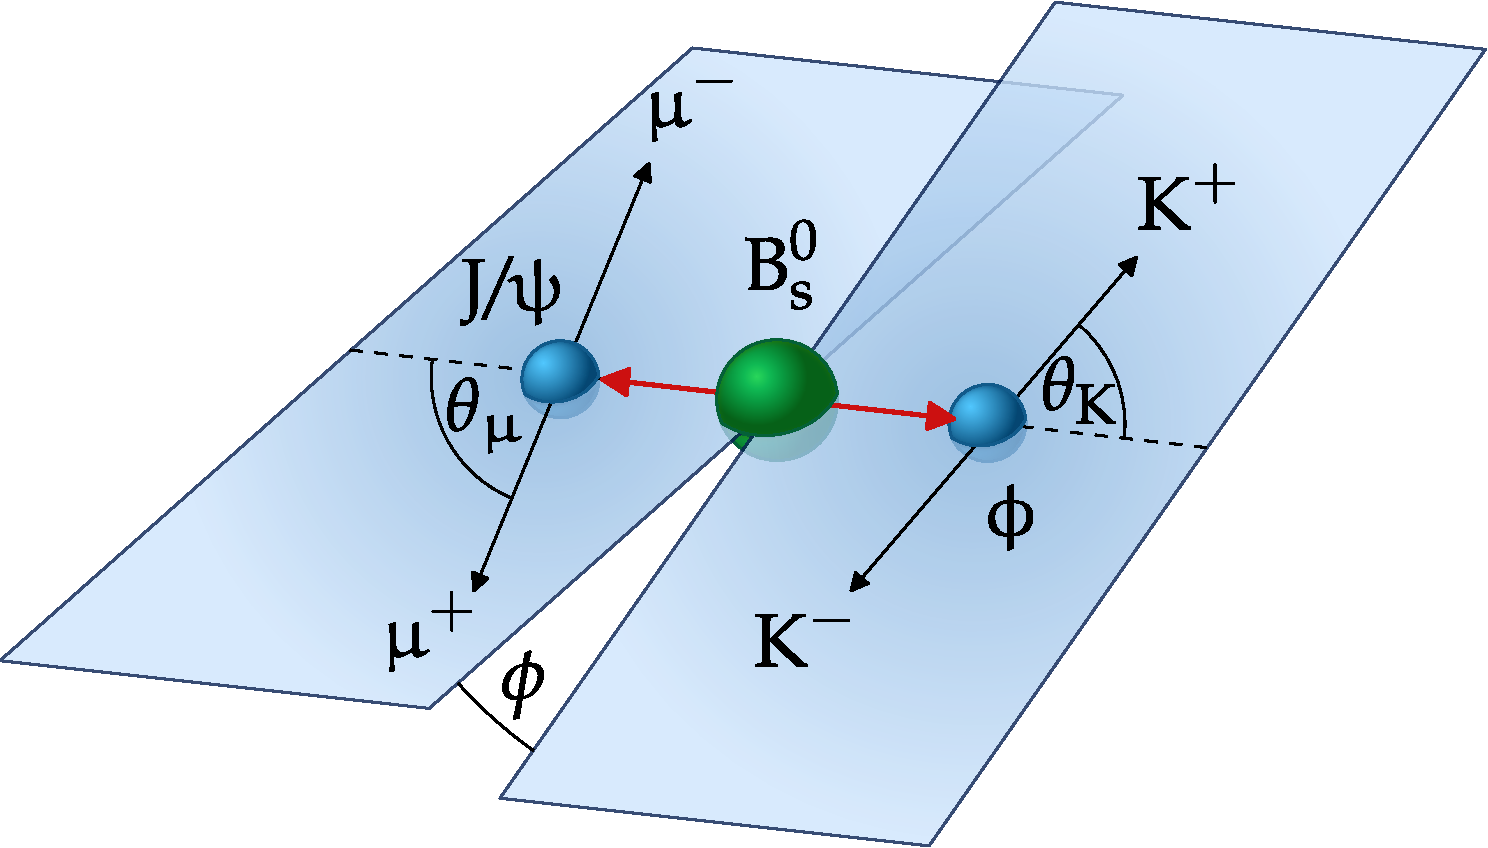
\includegraphics[width=0.7\textwidth]{HelicityPlanes.pdf}
\caption{Definición de los ángulos de helicidad.} \label{fig_angdist}
\end{figure}


Ahora conviene hacer una rotación a la base de las amplitudes de transversalidad, que son
\begin{equation}
\begin{array}{ccl}
\text{S}:& i=1 & \mathcal{A}_{\text{S}} = H_{0,0} \\ \\
  & i=2 & \mathcal{A}_{\perp} = \frac{\sqrt{2}}{2} (H_{1,+1}-H_{1,-1})   \\
\text{P}:& i=3 & \mathcal{A}_{0} = H_{1,0} \\
  & i=4 & \mathcal{A}_{\parallel} = \frac{\sqrt{2}}{2} (H_{1,+1}+H_{1,-1}) \\ \\
  & i=5 & \mathcal{A}_{2\perp} = \frac{\sqrt{2}}{2} (H_{2,+1}-H_{2,-1}) \\
\text{D}:& i=6 & \mathcal{A}_{20} = H_{2,0} \\
  & i=7 & \mathcal{A}_{2\parallel} = \frac{\sqrt{2}}{2} (H_{2,+1}+H_{2,-1})  
\end{array}	\label{eq:amps}
\end{equation}
que se corresponden con estados con autovalores de $\OPcp$ bien definidos. De este modo, la parte angular de la sección eficaz vendría dada por los coeficientes $\Omega_{ij}$ del Apéndice \ref{ap_angdistampana},
\begin{equation}
\frac{d^3 \Gamma}{d\cos\theta_{\text{K}} d\cos\theta_{\upmu} d\phi} \propto \sum_{i=1}^{7}  \sum_{j=1}^i N_{ij} \Omega_{ij}(\theta_{\upmu},\theta_{\text{K}},\phi).
\end{equation}


\begin{table}[H]
\centering
\begin{tabular}{c|ccc} 
\toprule
Onda & $\perp$ & $0$ & $\parallel$\\ 
\midrule
S &      & $-1$ &       \\
P & $-1$ & $+1$ & $+1$  \\
D & $+1$ & $-1$ & $-1$  \\ 
\bottomrule
\end{tabular}
\caption{Signatura, $\eta$, de los autovalores de $\OPcp$ para las amplitudes de transversalidad.}	
\end{table}

\begin{figure}[H]
\centering
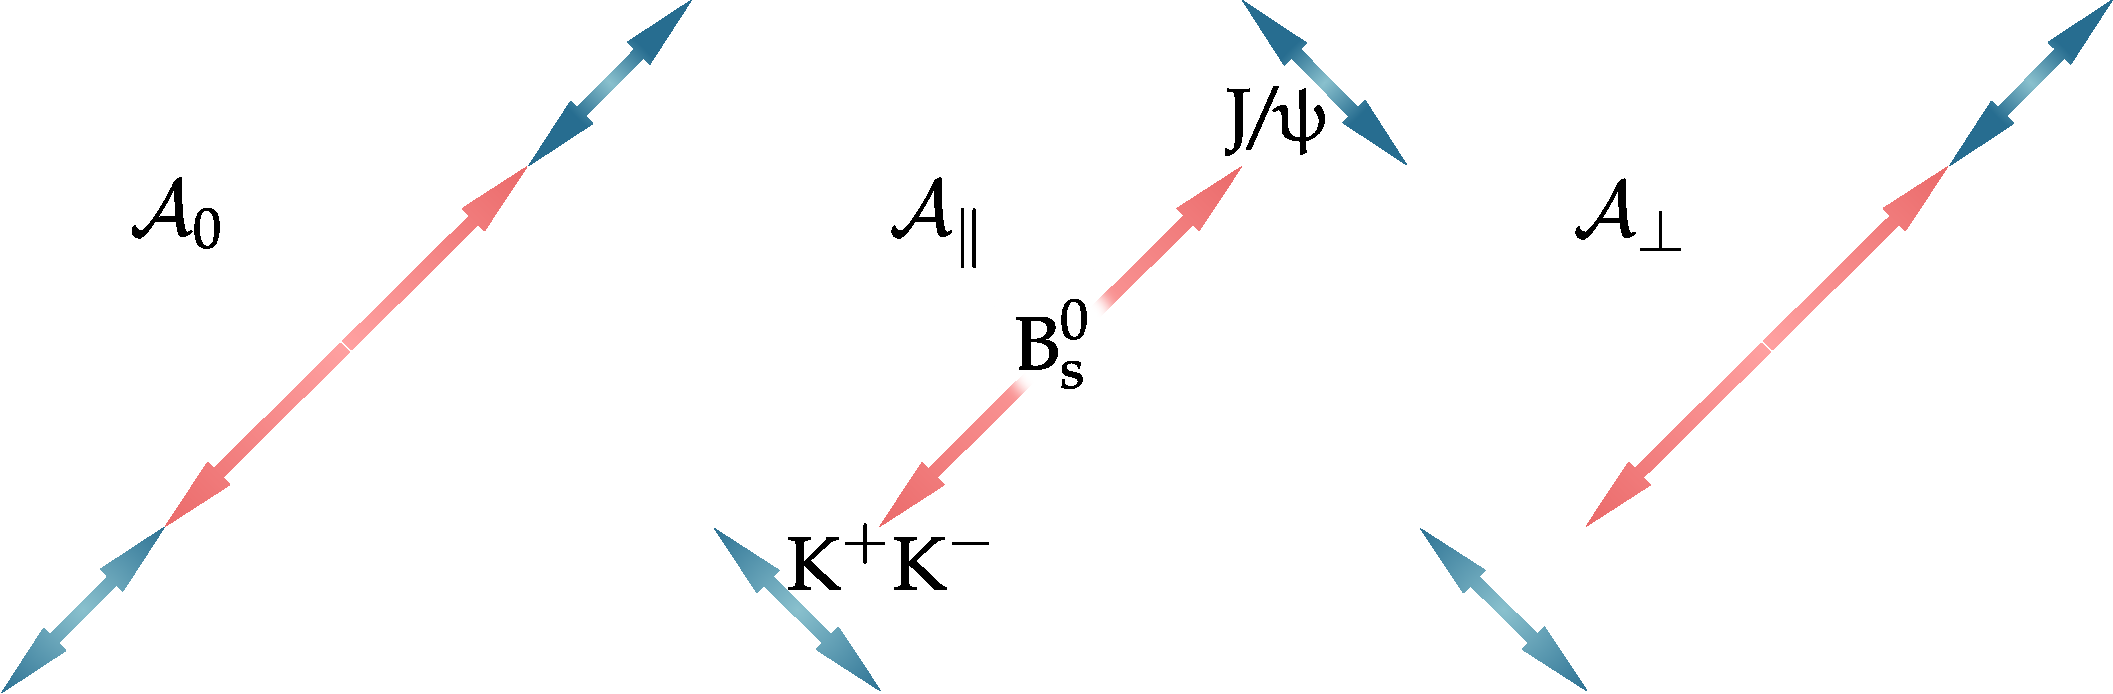
\includegraphics[width=0.8\textwidth]{HelicityPolarizations.pdf}
\caption{Configuraciones de polarización en la base de transversalidad.}
\end{figure}


\subsection{Dependencia temporal} %%%%%%%%%%%%%%%%%%%%%%%%%%%%%%%%%%%%%%%%%%%%%%
\label{sec_tempdist}

Como hemos visto en \S \ref{sec_evotempB}, debido a la mezcla $\Bs-\Bbs$, cada una de las amplitudes de polarización $\mathcal{A}_k$ se describe como
\begin{equation}
\mathcal{A}_k(t) = g_+ (t) \mathcal{A}{}_k^0 + \eta_k \frac{q}{p} g_{-}(t) \overline{\mathcal{A}}{}_f^0
\end{equation}
donde el superíndice $0$ indica que se trata de las amplitudes a $t=0$; $\eta_k$ es el signo del autovalor de $\OPcp$, dependiendo del comportamiento de la amplitud bajo paridad; $p$ y $q$ son parámetros que contiene la física del \emph{mixing}; y las funciones dependientes del tiempo $g_{\pm}(t)$ se corresponden con la Ecuación (\ref{eq_gedete}), verificándose además la relación entre las amplitudes 
\begin{equation}
	\frac{q}{p} \frac{\overline{\mathcal{A}}{}_k^0}{\mathcal{A}{}_k^0} = \eta_k e^{i {\varphi_s}_k}
\end{equation}
con $\varphi_s$ dada por la Ecuación (\ref{eq_phismixdecay}).


Centrándose solo en una contribución $k$, la tasa de desintegración dependiente del tiempo puede expresarse como
\begin{equation}
\begin{split}
\Gamma (t)  \propto e^{-\Gamma t} &\left[\frac{|A|^2+|\overline{A}|^2}{2} \cosh \left(\frac{\Delta \Gamma}{2} t \right) + \frac{|A|^2-|\overline{A}|^2}{2} \cos \left(\Delta m t \right) \right. - \\ & \left. \Re (A^* \overline{A}) \sinh \left(\frac{\Delta \Gamma}{2} t \right) - \Im (A^* \overline{A}) \sinh \left(\Delta m t\right) \right] \\
\overline{\Gamma} (t)  \propto e^{-\Gamma t} &\left[\frac{|A|^2+|\overline{A}|^2}{2} \cosh \left(\frac{\Delta \Gamma}{2} t \right) - \frac{|A|^2-|\overline{A}|^2}{2} \cos \left(\Delta m t \right) \right. - \\ & \left. \Re (A^* \overline{A}) \sinh \left(\frac{\Delta \Gamma}{2} t \right) + \Im (A^* \overline{A}) \sinh \left(\Delta m t\right) \right] 
\end{split}	 \label{eq_decayrateamp}
\end{equation}
o, previa definición de estos coeficientes (\emph{vid.} \ref{ap_angdistampana}),
\begin{equation}
\begin{split}
a_{ij} &= \AmpA_i(0) \AmpA_j^*(0) + \AmpAb_i (0) \AmpAb_j^* (0)\\
b_{ij} &= -\left(\AmpA_i(0) \AmpAb_j^*(0) + \AmpAb_i (0) \AmpA_j^* (0) \right)\\
c_{ij} &= \AmpA_i(0) \AmpA_j^*(0) - \AmpAb_i (0) \AmpAb_j^* (0)\\
d_{ij} &= -i \left(\AmpA_i(0) \AmpAb_j^*(0) - \AmpAb_i (0) \AmpA_j^* (0) \right).
\end{split}
\end{equation}
se puede convenientemente reescribir, para una población inicial de $\Bs$, como
\begin{equation}
	\frac{d\Gamma}{dt} \propto \sum_{i=1}^{7}\sum_{j=1}^i h_{ij}(t)
\end{equation}
donde las funciones dependientes del tiempo, $h_{ij}$, vienen dadas por 
\begin{equation}
\begin{split}
	h_{ij}(t) = e^{-\Gamma t} &\left[  a_{ij} \cosh \left(\frac{\Delta \Gamma}{2} t \right) + c_{ij} \cos \left(\Delta m t \right) \right. + \\ & \left. b_{ij} \sinh \left(\frac{\Delta \Gamma}{2} t \right) + d_{ij} \sinh \left(\Delta m t\right) \right]
\end{split}
\end{equation}
en donde, a la vista de la Ecuación (\ref{eq_decayrateamp}), se puede obtener la expresión para una población inicial de $\Bbs$, cambiando de signo los coeficientes $c_{ij}$ y $d_{ij}$.


Para distinguir mejor los términos susceptibles de violación CP, se escriben las amplitudes
\[\mathcal{A}_f^0 = \sqrt{1-\mathscr{A}_D} \, e^{-i \varphi_D} \, A_f^0, \qquad \overline{\mathcal{A}}_f^0 = \sqrt{1+\mathscr{A}_D} \, e^{i \varphi_D} \, A_f^0 \]
de modo que $\mathscr{A}_D $ es una CPV directa y $\varphi_D$ es una fase débil que da cuenta de la desintegración
\begin{equation}
	\mathscr{A}_D = \frac{|\mathcal{A}_f^0|^2-|\overline{\mathcal{A}}_f^0|^2}{|\mathcal{A}_f^0|^2+|\overline{\mathcal{A}}_f^0|^2}, \qquad \varphi_D = \frac{\text{arg}(\overline{\mathcal{A}}_f^0)-\text{arg}(\mathcal{A}_f^0)}{2}.
\end{equation}
%
La fase de interferencia entre el \textit{mixing} y el \emph{decay} es por tanto,
\begin{equation}
	\varphi_s \equiv \varphi_s^{\Jpsi KK} = \varphi_{M} + 2 \varphi_{D} \label{eq_phismixdecay}
\end{equation}
que junto con $|\lambda|$, son los parámetros que se pretenden medir con precisión en este análisis
\begin{equation}
|\lambda| = \frac{\sqrt{1+\mathscr{A}_D}}{\sqrt{1-\mathscr{A}_D}}	.
\end{equation}





%%%%%%%%%%%%%%%%%%%%%%%%%%%%%%%%%%%%%%%%%%%%%%%%%%%%%%%%%%%%%%%%%%%%%%%%%%%%%%%%
\section{Distribuciones de masa} %%%%%%%%%%%%%%%%%%%%%%%%%%%%%%%%%%%%%%%
% TODO cite ref 22 ananote


Como se decía en la \S \ref{sec_diffrate}, a la hora de parametrizar el espectro de masas en la región del $\fai(1020)$ se usan la propia resonancia $\fai$ de espín $1$ y la contribución de onda S  de espín $0$\footnote{La región de alta masa suele parametrizar $\ftwop$ (de espín $2$), aunque no afecta mucho en la ventana de masa que aquí se emplea.}. A continuación se describen las dependencias de masa junto con los \emph{barrier factors}. \todo{mejor así?}
%
\color{dieg}
En lo sucesivo se tomarán las masas,  $m_{*}$, y anchuras, $\Gamma_{*
}$, como las nominales de la Tabla \ref{tab_massPDG}.


%\color{rem}
%Esto es: $m_{\kaon} = m_{\antikaon} = 493.677$ MeV, $m_{\uppi^+} = m_{\uppi^-} = 139.57018$ MeV, $m_{\text{K}^0} = 497.614$ MeV, $m_{\uppi^0} = 134.9766$ MeV, $m_{\fzero} = 949.9$ MeV, $m_{\ftwop} = 1525$ MeV, $\Gamma_{\ftwop} = 73$ MeV, $m_{\fai} = 1019.4610$, $\Gamma_{\fai} = 4.266$ MeV, $m_{\Bs} = 5366.77$ MeV y $m_{\Jpsi} = 3096.916$ MeV. <CITE PDG>
\color{dieg}

\begin{table}[H]
  \centering
  \begin{tabular}{ccc}
\toprule
Partícula & $m \, (\text{MeV}/c^2)$  & $\Gamma$ \\ \midrule
$\mathrm{K^{\pm}}$    & $ 493.677\pm0.016 $\\
$\mathrm{K^{0}}$      & $497.611\pm0.013$\\
$\uppi^{\pm}$         & $139.57061\pm0.00024$\\
$\uppi^{0}$           & $134.9770\pm0.0005$\\
$\fai (1020)$         & $1019.461\pm0.016$  & $4.249\pm0.013 \, \text{MeV}$\\
$\Jpsi$               & $3096.900\pm0.006$  \\%& $92.9\pm2.8 \,\times 10^{-3}$
$\Bs$                 & $5366.89\pm0.19$ \\ \midrule
$\fzero (980)$        & $949.9\pm2.1$ \\
$\ftwop (1525)$       & $1522_{-3}^{+6}$          & $84_{-8}^{+12} \, \text{keV}$\\
\bottomrule
  \end{tabular}
  \caption{Masas nominales de partículas tomados de \cite[primer bloque]{pdg2018} y \cite[segundo bloque]{Aaij:1664567}.} \label{tab_massPDG}
\end{table}
\color{norm}


\color{new}
La amplitud $R(m)$ se usa para describir la \emph{line--shape} de masa de la resonancia $R$, en este caso correspondientes a $\fzero$, $\fai$ y $\ftwop$. Se combina esta función con las propiedades del decaimiento del $\Bs$, resultando la expresión \cite{Aaij:1664567}  
\begin{equation}
  \mathcal{M}_R = \sqrt{2 j + 1}\, \sqrt{q_m,q_{\Bs}} \,\mathfrak{B}_j \, R(m) \label{eq:masslineshape}
\end{equation}
siendo $j$ el espín de la resonancia, $\mathfrak{B}_j$ los \emph{barrier factors} y  $\sqrt{q_m,q_{\Bs}}$ el factor de espacio fásico, para tener en cuenta la cinemática de la desintegración a cuatro cuerpos se tiene que incluir una densidad de espacio fásico.
%
%TODO <meter algo más de palla>
%
%
% P
%
%
\color{norm}
%
El espacio fásico va a depender de los momentos $q_{\kaon}$  ($q_{\antikaon}$), momento del $\kaon$($\antikaon$) respecto del sistema en reposo $\kaon\antikaon$; y  $q_{\Bs}$, momento del sistema $\kaon\antikaon$ respecto del sistema en reposo del $\Bs$. Todos esos momentos se construyen de la forma:
\begin{equation}
q_m \equiv q(m,m_1,m_2) = \frac{1}{2}  \sqrt{m^2+\frac{\left(m_1^2-m_2^2\right){}^2}{m^2}-2 \left(m_1^2+m_2^2\right)}	
\end{equation}
y por lo tanto se definen $q_m \equiv q(m_R,m_{\kaon},m_{\antikaon})$, donde $m_R$ es la masa de la resonancia, y $q_{\Bs} \equiv q(m_{\Bs},m,m)$.



Los \emph{barrier factors} de momento angular se construyen como \cite{blatt2012theoretical}
\begin{equation}
\mathfrak{B}_j = \left[ B_{\ell}(q_{\Bs},\tilde{q}_{\kaon\antikaon}) \left( \frac{q_{\Bs}}{\tilde{q}_{\kaon\antikaon}} \right)^{\ell}\right] \, \left[ B_j(q_m,\tilde{q}_m) \left( \frac{q_m}{\tilde{q}_m} \right)^j\right]
\end{equation}
siendo $B_j(q,q0) \equiv B(j,q,q_0)$ los Blatt--Weisskopf \emph{barrier factors}, que hasta $j=2$ son:
\begin{equation} 
B_0 = 1, \qquad B_1 = \sqrt{\frac{1+(q_0d)^2}{1+(qd)^2}}, \qquad B_2 = \sqrt{\frac{9+3(q_0d)^2+(q_0d)^4}{9+3(qd)^2+(qd)^4}},
\end{equation}
donde el parámetro $d$ se corresponde con el tamaño característico de la partícula que decae y se mantiene fijo en $d = \frac{3\times10^{-3}}{j}$.



Para cada una de las contribuciones se emplea una resonancia $R(m)$, para lo que se hace uso de las siguientes distribuciones \cite{paperPhis}:

\paragraph{Distribución de Breit--Wigner}

Tanto la resonancia $\fai(1020)$, vectorial, como $\ftwop(1525)$, tensorial, se parametrizan con una función Breit--Wigner relativista que se define como: 
\begin{equation}
\mathcal{B}(m;m_0,\Gamma_0,m_1,m_2,j) = \frac{1}{(m_0^2-m^2)-im_0\Gamma(m;m_0,\Gamma_0,m_1,m_2,j)}
\end{equation}
La función $\Gamma(m;m_0,\Gamma_0,m_1,m_2,j)$, llamada \emph{running width}, viene dada por
\begin{equation}
	\Gamma(m;m_0,\Gamma_0,m_1,m_2,j) = \Gamma_0 \left(\frac{q_m}{q_0}\right)^{2j+1}\, \frac{m_0}{m} \, B_j (q_m,q_0)
\end{equation}


\paragraph{Distribución de Flatté}

Para la resonancia $\fzero(980)$, escalar,  se parametriza con una función Breit--Wigner relativista modificada, denominada distribución de Flatté, definida tal que así: 
\begin{equation}
\mathcal{F}(m;m_0) = \frac{1}{(m_0^2-m^2)-im_0(\Gamma_\text{K}+\Gamma_{\uppi})}
\end{equation}
siendo,
\begin{equation}
	\Gamma_{\text{K}} = \sqrt{1-\frac{m_{\text{K}}^2}{m^2}}, \qquad 	\Gamma_{\uppi} = \sqrt{1-\frac{m_{\uppi}^2}{m^2}}.
\end{equation}
La masa del polo del $\fzero(980)$ está muy cerca del umbral cinemático para decaer en dos kaones. Debido a las condiciones de unitariedad, este efecto distorsiona significativamente la forma del $\fzero$ en el espectro de masa de dos piones \cite{baru2005flatte}. \todo{qué tal así?}




%%%%%%%%%%%%%%%%%%%%%%%%%%%%%%%%%%%%%%%%%%%%%%%%%%%%%%%%%%%%%%%%%%%%%%%%%%%%%%%%
\subsection{Contribuciones de masa}

El espectro de masa $M_{\text{KK}}$ estará formado a lo sumo por tres componentes que se construirán con Ecuación \ref{eq:masslineshape} y los parámetros de la Tabla \ref{tab_massPDG}. Las formas de las ditribuciones y sus fases pueden verse en la Figura \ref{fig:masslineshape}, donde pueden apreciarse diferentes contribuciones dependiendo del la masa.

%TODO amañar pictures con python
\begin{figure}[H]
\centering
\subfloat[Resonancia de la masa $\fzero$ (azul) y distribución de la fase (verde).\label{fig_flatte}]{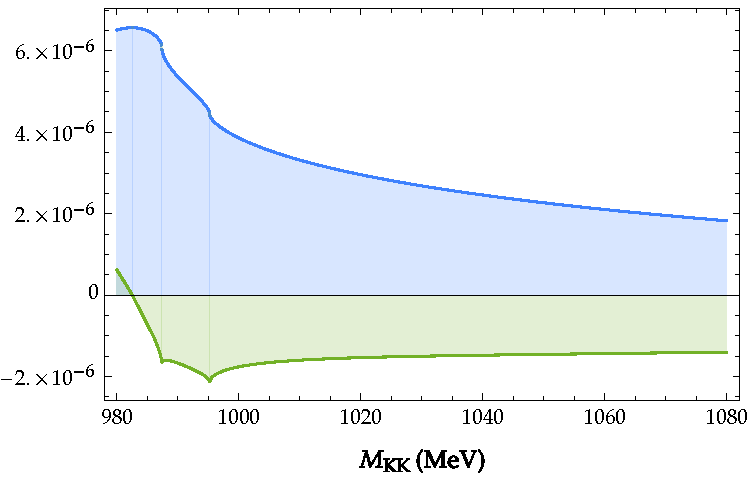
\includegraphics[width=0.48\textwidth]{flatte.pdf}} \hfill
\subfloat[Resonancia de la masa $\fai$ (azul) y distribución de la fase (verde).\label{fig_faires}]{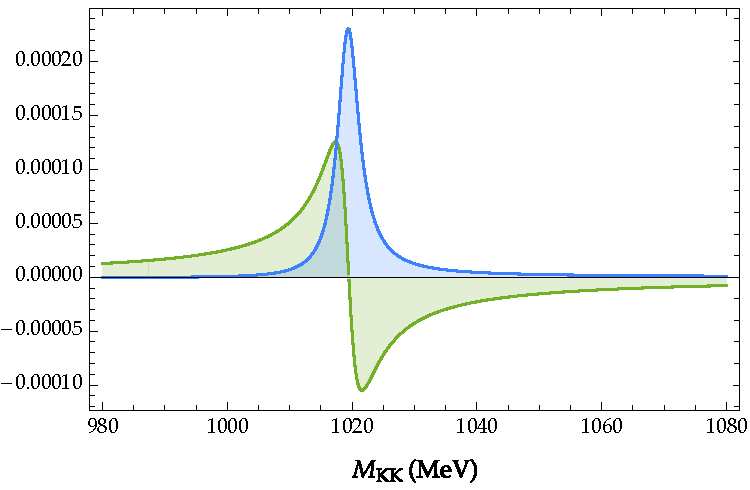
\includegraphics[width=0.48\textwidth]{BW_phi.pdf}} \hfill
\subfloat[Resonancia de la masa $\ftwop$ (azul) y distribución de la fase (verde).\label{fig_flatte}]{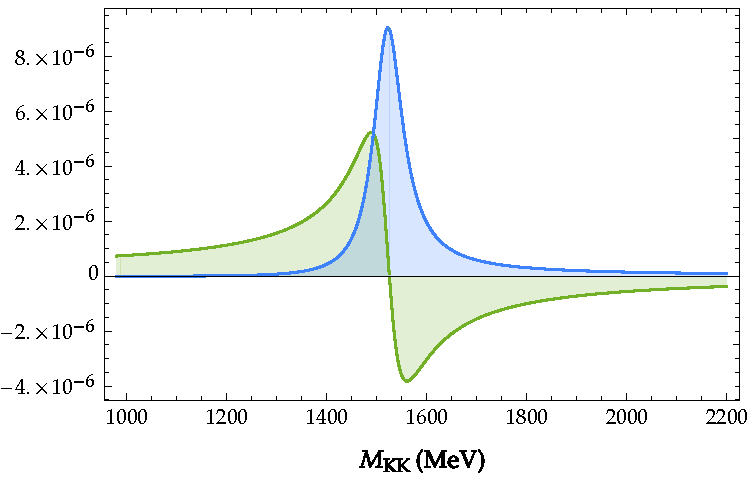
\includegraphics[width=0.48\textwidth]{BW_f2p.pdf}} \hfill
\subfloat[Espectro de masa KK con las resonacias $\fzero$ (naranja), $\fai$ (azul) y $\ftwop$ (rojo). Se hace uso de la escala logarítmica para poder distinguir las tres formas. \label{fig_mKK_linemass}]{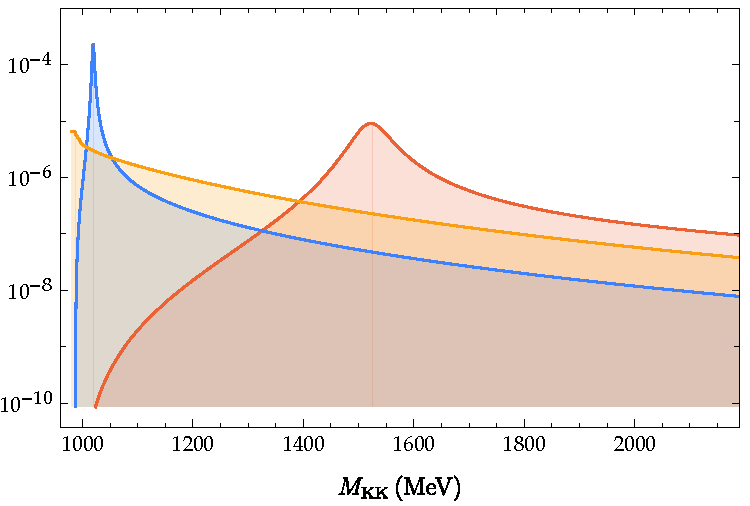
\includegraphics[width=0.48\textwidth]{mass_shape.pdf}} \hfill
\caption{Funciones de distribución de masa, para las 3 componentes resonantes estudiadas.}  \label{fig:masslineshape}
\end{figure}

\paragraph{Componente escalar $\bm{(j=0)}$}
Esta componente se supone la dominante en los rangos de masa $980- 1000$ MeV$/c^2$ y $1050-1400$ MeV$/c^2$ y se atribuye a una contribución de onda S resonante, correspondiente con el $\fzero(980)$. %, aunque también existe la posibilidad de añadir  S--\emph{wave}  no resonante.
La ausencia de un completo entendimiento de esta componente y de su relación con la la onda P, provoca que se haga un ajuste en diferentes bines de masa (\emph{vid.} \S \ref{sec_factorescspcspdcssd}). Esta componente se modela con una forma \todo{???}
\begin{equation}
	s(m) = \mathcal{F}(m;m_{\fzero}) \, \mathfrak{B}_0.
\end{equation}

\paragraph{Componente vectorial $\bm{(j=1)}$}
La componente principal de la ventana de masa es la correspondiente al $\fai(1020)$ de espín $1$. Para su modelado se emplea una Breit--Wigner relativista, quedando su \emph{line--shape}
\begin{equation}
	p(m) = \mathcal{B}(m;m_{\fai},\Gamma_{\fai},m_{\kaon},m_{\antikaon},1) \, \mathfrak{B}_1.
\end{equation}
Es la componente mayoritaria en el rango de masa $1000-1050$ MeV$/c^2$.


\paragraph{Componente tensorial $\text{(\textit{j}}\mathbf{=}\text{2)}$}
A pesar de que esta contribución es despreciable en la ventana de masa $[980,1200]$ MeV, la resonancia $\ftwop(1525)$ de espín $2$ también hace uso de una BW,
\begin{equation}
	d(m) = \mathcal{B}(m;m_{\ftwop},\Gamma_{\ftwop},m_{\kaon},m_{\antikaon},1) \, \mathfrak{B}_2.
\end{equation}
Su preeminencia se sitúa en el rango de masa $1400-2200$ MeV$/c^2$.




%%%%%%%%%%%%%%%%%%%%%%%%%%%%%%%%%%%%%%%%%%%%%%%%%%%%%%%%%%%%%%%%%%%%%%%%%%%%%%%%
%\subsection[ee]{Factores 
%\begingroup
%\fontfamily{newtxsf}\selectfont\bfseries\sffamily\sansmath
%$C_{\text{SP}}$, $\bm{C_{\text{SD}}}$ y $\bm{C_{\text{PD}}}$
%\endgroup
%} %%%%%%

\subsection{Factores 
$\text{\textit{C}}_{\text{SP}}$, $\text{\textit{C}}_{\text{SD}}$ y $\text{\textit{C}}_{\text{PD}}$
}

\label{sec_factorescspcspdcssd}
%TODO bold math

En la Tabla \ref{tab_coeffsfk}, a las contribuciones correspondientes a interferencia entre las amplitudes, las acompañan los factores $C_{\text{SP}}$, $C_{\text{SD}}$ y $C_{\text{PD}}$ , que dan cuenta del cambio relativo de fracciones de las diferentes polarizaciones en los bines de masa $m_{\text{KK}}$.

Para poder calcular estos factores, se deben explicitar las expresiones analíticas de las funciones de forma normalizadas de la masas  $s(m_{\text{KK}})$ (onda S), $p(m_{\text{KK}})$ (onda P)  y $d(m_{\text{KK}})$ (onda D). El problema nace principalmente porque $\langle p \times s^* \rangle \neq \langle p \rangle \langle s^* \rangle$ (e igual para los demás factores) \cite{Xie:1461783}. Entonces para cada bin $m_{\text{KK}}$, se integra  
\begin{equation}
C_{\text{SP}} e^{-i \theta_{\text{SP}}} =
\frac{\int_{m_{KK}^L}^{m_{KK}^H} { p(m_{KK}) \times s(m_{KK})^*} \:\:d m_{KK}}
{\sqrt{\int_{m_{KK}^L}^{m_{KK}^H} { |p(m_{KK})|^2}  \:\:d m_{KK} \,\,\int_{m_{KK}^L}^{m_{KK}^H} { |s(m_{KK})|^2}  \:\:d m_{KK}}}
\end{equation}
y análogamente para los demás factores de corrección.
\todo{more on this?}


\begin{table}[H]
\centering
\begin{tabular}{c|c}
\toprule
$m_{\text{KK}}$ GeV & $C_{\text{SP}}$ \\ \midrule
$[0.990,1.008]$ & 0.8463  \\
$(1.008,1.016]$ & 0.8756  \\
$(1.016,1.020]$ & 0.8478  \\
$(1.020,1.024]$ & 0.8833  \\
$(1.024,1.032]$ & 0.9415  \\
$(1.032,1.050]$ & 0.9756  \\
\bottomrule
\end{tabular}
\caption{Factores de corrección para los bines de masa KK definidos en la región del $\fai(1020)$.}	
\end{table}


\begin{table}[H]
\centering
\begin{tabular}{c|ccc}
\toprule
$m_{\text{KK}}$ GeV & $C_{\text{SP}}$ & $C_{\text{SD}}$ & $C_{\text{PD}}$\\ \midrule
$[1.0,1.2]$ & 0.8420 & 0.8525 & 0.9965 \\
$(1.2,1.4]$ & 0.9273 & 0.9925 & 0.9623 \\
$(1.4,1.6]$ & 0.9053 & 0.9987 & 0.9122 \\
$(1.6,1.8]$ & 0.9485 & 0.9990 & 0.9372 \\
$(1.8,2.0]$ & 0.9734 & 0.9969 & 0.9531 \\
$(2.0,2.2]$ & 0.9840 & 0.9901 & 0.9499 \\
\bottomrule
\end{tabular}
\caption{Factores de corrección para los bines de masa KK definidos en la ventana de masa $[1.0,2.2]$ GeV$/c^2$.}	
\end{table}





%%%%%%%%%%%%%%%%%%%%%%%%%%%%%%%%%%%%%%%%%%%%%%%%%%%%%%%%%%%%%%%%%%%%%%%%%%%%%%%%
%%%%%%%%%%%%%%%%%%%%%%%%%%%%%%%%%%%%%%%%%%%%%%%%%%%%%%%%%%%%%%%%%%%%%%%%%%%%%%%%
%%%%%%%%%%%%%%%%%%%%%%%%%%%%%%%%%%%%%%%%%%%%%%%%%%%%%%%%%%%%%%%%%%%%%%%%%%%%%%%%

\bigskip

\begin{center}
	$***$
\end{center}

\medskip

%%%%%%%%%%%%%%%%%%%%%%%%%%%%%%%%%%%%%%%%%%%%%%%%%%%%%%%%%%%%%%%%%%%%%%%%%%%%%%%%
%%%%%%%%%%%%%%%%%%%%%%%%%%%%%%%%%%%%%%%%%%%%%%%%%%%%%%%%%%%%%%%%%%%%%%%%%%%%%%%%
%%%%%%%%%%%%%%%%%%%%%%%%%%%%%%%%%%%%%%%%%%%%%%%%%%%%%%%%%%%%%%%%%%%%%%%%%%%%%%%%

\begin{subappendices}

%\titleformat{\section} 
%  {\normalfont}{\spacedlowsmallcaps\appendixname\ %
%  {\spacedallcaps\thesection}}%
%  {1em}{\spacedallcaps}

%%%%%%%%%%%%%%%%%%%%%%%%%%%%%%%%%%%%%%%%%%%%%%%%%%%%%%%%%%%%%%%%%%%%%%%%%%%%%%%%



%%%%%%%%%%%%%%%%%%%%%%%%%%%%%%%%%%%%%%%%%%%%%%%%%%%%%%%%%%%%%%%%%%%%%%%%%%%%%%%%
%Matrices Wigner
%%%%%%%%%%%%%%%%%%%%%%%%%%%%%%%%%%%%%%%%%%%%%%%%%%%%%%%%%%%%%%%%%%%%%%%%%%%%%%%%
%%%%%%%%%%%%%%%%%%%%%%%%%%%%%%%%%%%%%%%%%%%%%%%%%%%%%%%%%%%%%%%%%%%%%%%%%%%%%%%%
%%%%%%%%%%%%%%%%%%%%%%%%%%%%%%%%%%%%%%%%%%%%%%%%%%%%%%%%%%%%%%%%%%%%%%%%%%%%%%%%
\section{Matrices de Wigner}
\label{app_matwig}
%%%%%%%%%%%%%%%%%%%%%%%%%%%%%%%%%%%%%%%%%%%%%%%%%%%%%%%%%%%%%%%%%%%%%%%%%%%%%%%%
%%%%%%%%%%%%%%%%%%%%%%%%%%%%%%%%%%%%%%%%%%%%%%%%%%%%%%%%%%%%%%%%%%%%%%%%%%%%%%%%
%%%%%%%%%%%%%%%%%%%%%%%%%%%%%%%%%%%%%%%%%%%%%%%%%%%%%%%%%%%%%%%%%%%%%%%%%%%%%%%%



%%%%%%%%%%%%%%%%%%%%%%%%%%%%%%%%%%%%%%%%%%%%%%%%%%%%%%%%%%%%%%%%%%%%%%%%%%%%%%%%
%\section{Introducción } %%%%%%%%%%%%%%%%%%%%%%%%%%%%%%%%%%%%%%%%%%%%%%%%%%%%%%%%

Se denominan funciones $D$ de Wigner, $D_{m,m'}^j(\alpha,\beta,\gamma)$, a los elementos de matriz del operador de rotaciones, $R(\alpha,\beta,\gamma)$, para un estado $|j\,m\rangle$ con valores bien definidos de momento angular $j^2$ y de su proyección $j_z$ \cite{kutschke1996angular}. De modo que
\begin{equation}
	\psi_{jm'}(\theta',\phi',\sigma') = R(\Omega) \psi_{jm} (\theta,\phi,\sigma) = \sum_{m' = -j}^j  \psi_{jm} (\theta,\phi,\sigma) D_{m,m'}^j(\Omega),
\end{equation}
siendo $\theta$ y $\phi \, (\theta'$ y $\phi')$ los ángulos polares iniciales (rotados) y $\sigma(\sigma')$ referida a las variables de espín. Además, se tiene la relación con las matrices $d$ de Wigner,
\begin{equation}
	D_{m,m'}^j (\alpha,\beta,\gamma) \equiv e^{-i\alpha m} d_{m,m'}^j (\beta) e^{-i\gamma m'}.
\end{equation}


Al considerar la desintegración del $\Bs$ en $\Jpsi$ y $\fai$, que a su vez decaen en $\muon \antimuon$ y  $\kaon \antikaon$ \footnote{Aunque los nombres de partículas sean específicos, este es un marco y procedimiento general para las desintegraciones a cuatro cuerpos que mediados por dos resonancias intermedias para desintegraciones escalares.}.
%
Los estados para las partículas se definen, por ejemplo, para el $\Jpsi$, como $\Jpsi:  |j_{\Jpsi} \,\lambda_{\Jpsi}\rangle$. Cuando $\Jpsi$ decae, se proyecta en un nuevo plano, $X_{\Jpsi}',Y_{\Jpsi}',Z_{\Jpsi}'$, cuya amplitud es proporcional a 
\begin{equation*}
\langle j_{\Jpsi},\, \lambda_{\muon} - \lambda_{\antimuon} | R(\alpha,\beta,\gamma) | j_{\Jpsi} , \lambda_{\Jpsi} \rangle \equiv D_{\lambda_{\Jpsi},\lambda_{\muon} - \lambda_{\antimuon}}^{j_{\Jpsi}}	(\alpha,\beta,\gamma)
\end{equation*}
es decir, precisamente la matriz de Wigner-$D$. Aquí $\alpha,\beta$ y $\gamma$
son los ángulos de Euler, que en la Mecánica Clásica  definen cualquier posible rotación en el espacio tridimensional. Hay otras convenciones posibles para estos ángulos, una de ellas --- y la usada por \lhcb --- es la convención de Jacobi--Wick \cite{kutschke1996angular}, que dicta
$R(\alpha,\beta,\gamma)  \rightarrow R(\alpha,\beta,-\alpha).  $


\begin{figure}[H]
\centering
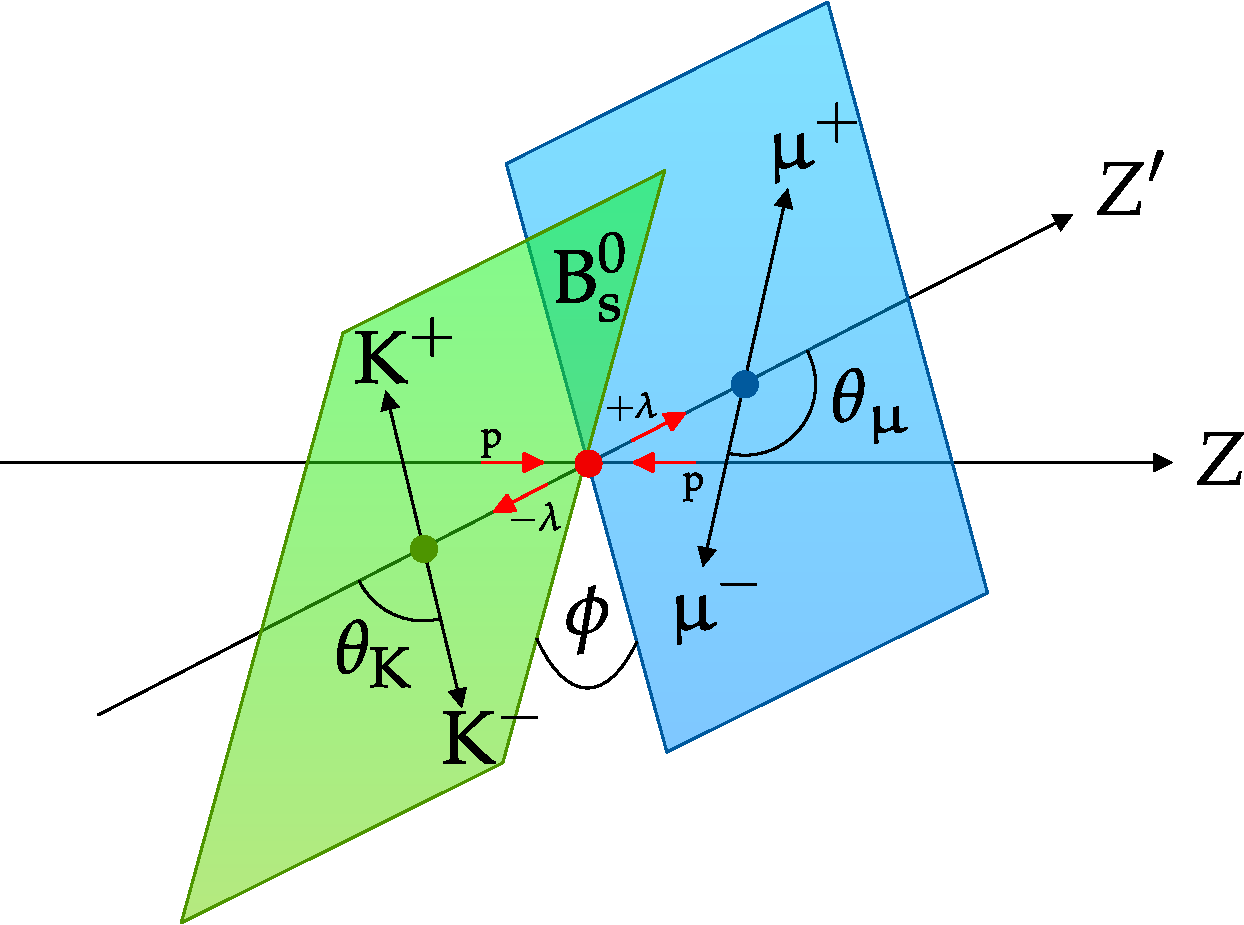
\includegraphics[width=0.48\textwidth]{WignerD1}
\hfill
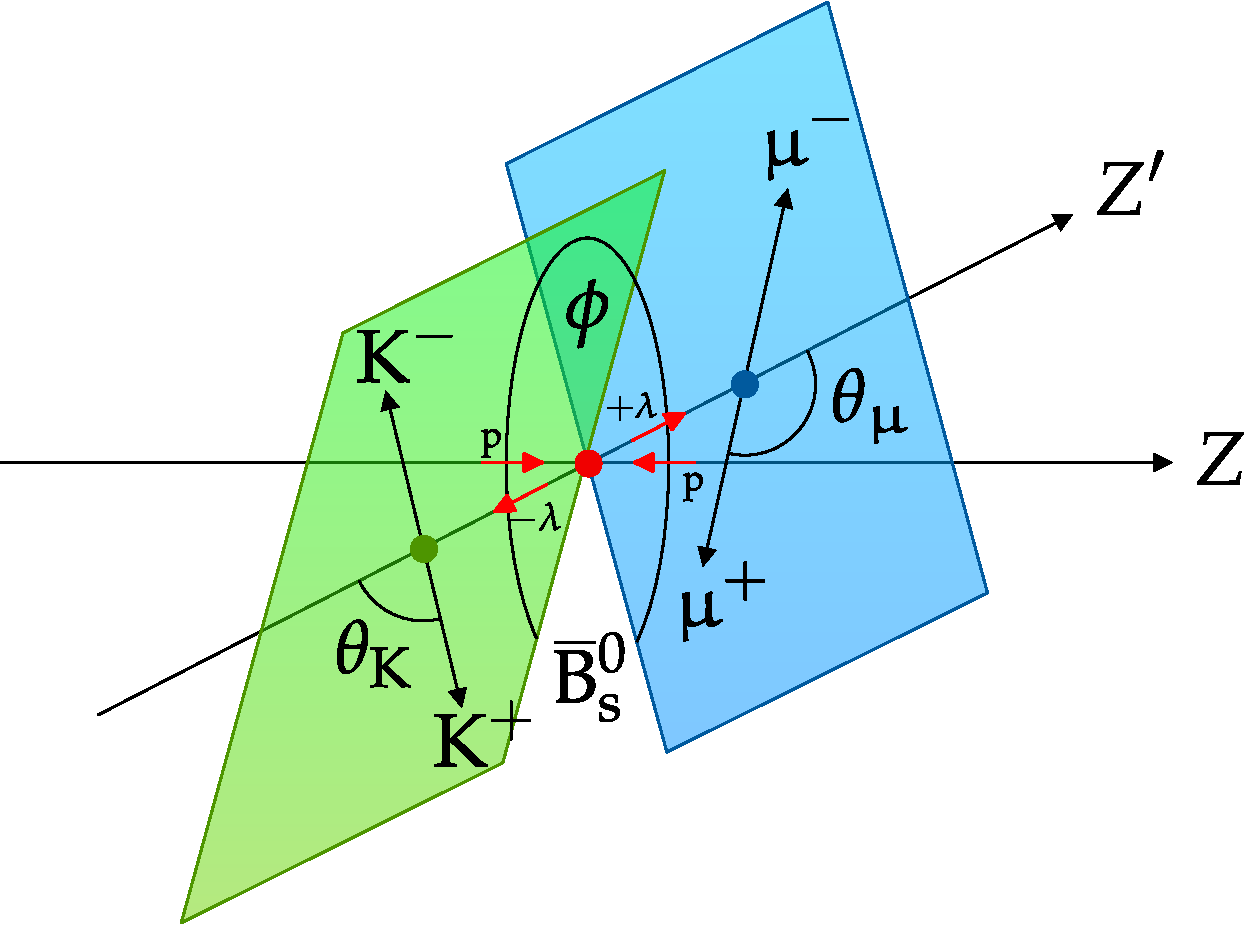
\includegraphics[width=0.48\textwidth]{WignerD2}
\caption{Definición de la helicidad y ángulos de helicidad para los desintegraciones $\Bs$ y $\Bbs$.}	
\end{figure}



%
Por tanto, la amplitud del proceso será proporcional al siguiente producto de funciones de Wigner
\[\mathcal{A} \sim D_{\lambda_{\Bs},\lambda_{\Jpsi}-\lambda_{\fai}}^{j_{\Bs}}\,D_{\lambda_{\Jpsi},\lambda_{\muon}-\lambda_{\antimuon}}^{j_{\Jpsi}}\, D_{\lambda_{\fai},\lambda_{\kaon}-\lambda_{\antikaon}}^{j_{\fai}}\]
Dado que el $\Bs$ carece de espín, $D_{0,\lambda_{\Jpsi}-\lambda_{\fai}}^0 = \delta_{0,\lambda_{\Jpsi}-\lambda_{\fai}}^0$, por lo que las helicidades del $\Jpsi$ y del $\fai$ deben ser contrarias respecto de la dirección del $\Bs$ (o equivalentemente, conservar el momento lineal). Así,
\[\mathcal{A} \sim D_{\lambda_{\Jpsi},\lambda_{\muon}-\lambda_{\antimuon}}^{j_{\Jpsi}}\, D_{\lambda_{\fai},\lambda_{\kaon}-\lambda_{\antikaon}}^{j_{\fai}},\]
o denominando $\lambda \equiv \lambda_{\Jpsi} = - \lambda_{\fai} $, $\alpha = \lambda_{\muon}-\lambda_{\antimuon}$, $j \equiv j_{\fai}$ y como los kaones son escalares \cite{zhang2013time},
\begin{equation}
\begin{split}
\mathcal{A} &  \sim D_{\lambda,\alpha}^{1}(0, \theta_{\upmu}, 0)\, D_{-\lambda,0}^{j} (\phi, \theta_{\text{K}} , -\phi ) = \\
&= d_{\lambda,\alpha}^{1} (\theta_{\upmu})\, e^{-i (-\lambda) (\phi)} d_{-\lambda,0}^{j}(\theta_{\text{K}}) e^{-i (0) (-\phi)} = \\ 
&= e^{i\lambda \phi} \,d_{\lambda,\alpha}^{1} (\theta_{\upmu})\,  d_{-\lambda,0}^{j}(\theta_{\text{K}}) .
\end{split}	
\end{equation}
encontrando así la notación estándar de los términos angulares de la amplitud.



%%%%%%%%%%%%%%%%%%%%%%%%%%%%%%%%%%%%%%%%%%%%%%%%%%%%%%%%%%%%%%%%%%%%%%%%%%%%%%%%
%%%%%%%%%%%%%%%%%%%%%%%%%%%%%%%%%%%%%%%%%%%%%%%%%%%%%%%%%%%%%%%%%%%%%%%%%%%%%%%%
%%%%%%%%%%%%%%%%%%%%%%%%%%%%%%%%%%%%%%%%%%%%%%%%%%%%%%%%%%%%%%%%%%%%%%%%%%%%%%%%



%%%%%%%%%%%%%%%%%%%%%%%%%%%%%%%%%%%%%%%%%%%%%%%%%%%%%%%%%%%%%%%%%%%%%%%%%%%%%%%%
\section{Coeficientes del análisis angular de amplitudes}
\label{ap_angdistampana}

Se presentan en forma de tabla los coeficientes de la sección eficaz diferencial desarrollada en el Capítulo \ref{cha:pheno}.




\begin{table}
\centering
\begin{tabular}{LC}
\toprule
\multicolumn{1}{c}{$N_{ij}$} & \Omega_{ij} \\
\midrule
\phantom{C_{\mathrm{SP}}} A_{\text{S}}^2 & \frac{1}{3} \sin ^2\left(\theta _{\mu }\right) \\
 C_{\mathrm{SP}} A_{\text{S}} A_{\perp} & \frac{\sin (\phi ) \sin \left(\theta _K\right) \sin \left(2 \theta _{\mu }\right)}{\sqrt{6}} \\
 \phantom{C_{\mathrm{SP}}} A_{\perp}^2 & \frac{1}{2} \left(\cos ^2(\phi )+\cos ^2\left(\theta _{\mu }\right) \sin ^2(\phi )\right) \sin ^2\left(\theta _K\right) \\
 C_{\mathrm{SP}} A_{\text{S}} A_{0} & \frac{2 \cos \left(\theta _K\right) \sin ^2\left(\theta _{\mu }\right)}{\sqrt{3}} \\
 \phantom{C_{\mathrm{SP}}} A_{\perp} A_{0} & -\frac{\sin (\phi ) \sin \left(2 \theta _K\right) \sin \left(2 \theta _{\mu }\right)}{2 \sqrt{2}} \\
 \phantom{C_{\mathrm{SP}}} A_{0}^2 & \cos ^2\left(\theta _K\right) \sin ^2\left(\theta _{\mu }\right) \\
 C_{\mathrm{SP}} A_{\text{S}} A_{\parallel} & \frac{\cos (\phi ) \sin \left(\theta _K\right) \sin \left(2 \theta _{\mu }\right)}{\sqrt{6}} \\
 \phantom{C_{\mathrm{SP}}} A_{\perp} A_{\parallel} & \frac{1}{2} \sin (2 \phi ) \sin ^2\left(\theta _K\right) \sin ^2\left(\theta _{\mu }\right) \\
 \phantom{C_{\mathrm{SP}}} A_{0} A_{\parallel} & \frac{\cos (\phi ) \sin \left(2 \theta _K\right) \sin \left(2 \theta _{\mu }\right)}{2 \sqrt{2}} \\
 \phantom{C_{\mathrm{SP}}} A_{\parallel}^2 & \frac{1}{2} \left(\cos ^2(\phi ) \cos ^2\left(\theta _{\mu }\right)+\sin ^2(\phi )\right) \sin ^2\left(\theta _K\right) \\
 C_{\mathrm{SD}} A_{\text{S}} A_{2\perp} & \frac{1}{2} \sqrt{\frac{5}{6}} \sin (\phi ) \sin \left(2 \theta _K\right) \sin \left(2 \theta _{\mu }\right) \\
 C_{\mathrm{PD}} A_{\perp} A_{2\perp} & \frac{1}{2} \sqrt{5} \left(\cos ^2(\phi )+\cos ^2\left(\theta _{\mu }\right) \sin ^2(\phi )\right) \sin \left(\theta _K\right) \sin \left(2 \theta _K\right) \\
 C_{\mathrm{PD}} A_{0} A_{2\perp} & \sqrt{\frac{5}{2}} \cos ^2\left(\theta _K\right) \sin (\phi ) \sin \left(\theta _K\right) \sin \left(2 \theta _{\mu }\right) \\
 C_{\mathrm{PD}} A_{\parallel} A_{2\perp} & -\frac{1}{2} \sqrt{5} \cos \left(\theta _K\right) \sin (2 \phi ) \sin ^2\left(\theta _K\right) \sin ^2\left(\theta _{\mu }\right) \\
 \phantom{C_{\mathrm{SP}}} A_{2\perp}^2 & \frac{5}{8} \left(\cos ^2(\phi )+\cos ^2\left(\theta _{\mu }\right) \sin ^2(\phi )\right) \sin ^2\left(2 \theta _K\right) \\
 C_{\mathrm{SD}} A_{\text{S}} A_{20} & \frac{1}{6} \sqrt{5} \left(3 \cos \left(2 \theta _K\right)+1\right) \sin ^2\left(\theta _{\mu }\right) \\
 C_{\mathrm{PD}} A_{\perp} A_{20} & -\frac{1}{4} \sqrt{\frac{5}{6}} \left(3 \cos \left(2 \theta _K\right)+1\right) \sin (\phi ) \sin \left(\theta _K\right) \sin \left(2 \theta _{\mu }\right) \\
 C_{\mathrm{PD}} A_{0} A_{20} & \frac{1}{2} \sqrt{\frac{5}{3}} \cos \left(\theta _K\right) \left(3 \cos \left(2 \theta _K\right)+1\right) \sin ^2\left(\theta _{\mu }\right) \\
 C_{\mathrm{PD}} A_{\parallel} A_{20} & \frac{1}{4} \sqrt{\frac{5}{6}} \cos (\phi ) \left(3 \cos \left(2 \theta _K\right)+1\right) \sin \left(\theta _K\right) \sin \left(2 \theta _{\mu }\right) \\
 \phantom{C_{\mathrm{SP}}} A_{2\perp} A_{20} & -\frac{5 \left(3 \cos \left(2 \theta _K\right)+1\right) \sin (\phi ) \sin \left(2 \theta _K\right) \sin \left(2 \theta _{\mu }\right)}{8 \sqrt{6}} \\
 \phantom{C_{\mathrm{SP}}} A_{20}^2 & \frac{5}{48} \left(3 \cos \left(2 \theta _K\right)+1\right){}^2 \sin ^2\left(\theta _{\mu }\right) \\
 C_{\mathrm{SD}} A_{\text{S}} A_{2\parallel} & \frac{1}{2} \sqrt{\frac{5}{6}} \cos (\phi ) \sin \left(2 \theta _K\right) \sin \left(2 \theta _{\mu }\right) \\
 C_{\mathrm{PD}} A_{\perp} A_{2\parallel} & \frac{1}{2} \sqrt{5} \cos \left(\theta _K\right) \sin (2 \phi ) \sin ^2\left(\theta _K\right) \sin ^2\left(\theta _{\mu }\right) \\
 C_{\mathrm{PD}} A_{0} A_{2\parallel} & \sqrt{\frac{5}{2}} \cos (\phi ) \cos ^2\left(\theta _K\right) \sin \left(\theta _K\right) \sin \left(2 \theta _{\mu }\right) \\
 C_{\mathrm{PD}} A_{\parallel} A_{2\parallel} & \frac{1}{2} \sqrt{5} \left(\cos ^2(\phi ) \cos ^2\left(\theta _{\mu }\right)+\sin ^2(\phi )\right) \sin \left(\theta _K\right) \sin \left(2 \theta _K\right) \\
 \phantom{C_{\mathrm{SP}}} A_{2\perp} A_{2\parallel} & \frac{5}{8} \sin (2 \phi ) \sin ^2\left(2 \theta _K\right) \sin ^2\left(\theta _{\mu }\right) \\
 \phantom{C_{\mathrm{SP}}} A_{20} A_{2\parallel} & \frac{5 \cos (\phi ) \left(3 \cos \left(2 \theta _K\right)+1\right) \sin \left(2 \theta _K\right) \sin \left(2 \theta _{\mu }\right)}{8 \sqrt{6}} \\
\phantom{C_{\mathrm{SP}}}  A_{2\parallel}^2 & \frac{5}{8} \left(\cos ^2(\phi ) \cos ^2\left(\theta _{\mu }\right)+\sin ^2(\phi )\right) \sin ^2\left(2 \theta _K\right) \\
 \bottomrule
\end{tabular}
\caption{Coeficientes $N_{ij}$ y $\Omega_{ij}$ de la distribución angular de la desintragración $\Bs \rightarrow \Jpsi \antikaon\kaon$ con las contribuciones de onda S, P y D.}	 \label{tab_coeffsfk}
\end{table}



\begin{table}
\centering
%\resizebox{\textwidth}{!}{
\begin{tabular}{CCC}
\toprule
i & j & a_{ij} \\
\midrule
 1 & 1 & \frac{1}{2} \left(\lambda _{\text{S}}^2+1\right) \\
 2 & 1 & \frac{1}{2} \left(\sin \left(\delta _{\text{S}}-\delta _{\perp}\right)+\sin \left(\delta _{\text{S}}-\delta _{\perp}-\varphi _{\text{S}}+\varphi _{\perp}\right) \lambda _{\text{S}} \lambda _{\perp}\right) \\
 2 & 2 & \frac{1}{2} \left(\lambda _{\perp}^2+1\right) \\
 3 & 1 & \frac{1}{2} \left(\cos \left(\delta _{\text{S}}-\delta _{0}\right)-\cos \left(\delta _{\text{S}}-\delta _{0}-\varphi _{\text{S}}+\varphi _{0}\right) \lambda _{\text{S}} \lambda _{0}\right) \\
 3 & 2 & \frac{1}{2} \left(\sin \left(\delta _{\perp}-\delta _{0}\right)-\sin \left(\delta _{\perp}-\delta _{0}-\varphi _{\perp}+\varphi _{0}\right) \lambda _{\perp} \lambda _{0}\right) \\
 3 & 3 & \frac{1}{2} \left(\lambda _{0}^2+1\right) \\
 4 & 1 & \frac{1}{2} \left(\cos \left(\delta _{\text{S}}-\delta _{\parallel}\right)-\cos \left(\delta _{\text{S}}-\delta _{\parallel}-\varphi _{\text{S}}+\varphi _{\parallel}\right) \lambda _{\text{S}} \lambda _{\parallel}\right) \\
 4 & 2 & \frac{1}{2} \left(\sin \left(\delta _{\perp}-\delta _{\parallel}\right)-\sin \left(\delta _{\perp}-\delta _{\parallel}-\varphi _{\perp}+\varphi _{\parallel}\right) \lambda _{\perp} \lambda _{\parallel}\right) \\
 4 & 3 & \frac{1}{2} \left(\cos \left(\delta _{0}-\delta _{\parallel}\right)+\cos \left(\delta _{0}-\delta _{\parallel}-\varphi _{0}+\varphi _{\parallel}\right) \lambda _{0} \lambda _{\parallel}\right) \\
 4 & 4 & \frac{1}{2} \left(\lambda _{\parallel}^2+1\right) \\
 5 & 1 & \frac{1}{2} \left(\cos \left(\delta _{\text{S}}-\delta _{2\perp}\right)+\cos \left(\delta _{\text{S}}-\delta _{2\perp}-\varphi _{\text{S}}+\varphi _{2\perp}\right) \lambda _{\text{S}} \lambda _{2\perp}\right) \\
 5 & 2 & \frac{1}{2} \left(\sin \left(\delta _{\perp}-\delta _{2\perp}\right)+\sin \left(\delta _{\perp}-\delta _{2\perp}-\varphi _{\perp}+\varphi _{2\perp}\right) \lambda _{\perp} \lambda _{2\perp}\right) \\
 5 & 3 & \frac{1}{2} \left(\cos \left(\delta _{0}-\delta _{2\perp}\right)-\cos \left(\delta _{0}-\delta _{2\perp}-\varphi _{0}+\varphi _{2\perp}\right) \lambda _{0} \lambda _{2\perp}\right) \\
 5 & 4 & \frac{1}{2} \left(\cos \left(\delta _{\parallel}-\delta _{2\perp}\right)-\cos \left(\delta _{\parallel}-\delta _{2\perp}-\varphi _{\parallel}+\varphi _{2\perp}\right) \lambda _{\parallel} \lambda _{2\perp}\right) \\
 5 & 5 & \frac{1}{2} \left(\lambda _{2\perp}^2+1\right) \\
 6 & 1 & \frac{1}{2} \left(\sin \left(\delta _{\text{S}}-\delta _{20}\right)-\sin \left(\delta _{\text{S}}-\delta _{20}-\varphi _{\text{S}}+\varphi _{20}\right) \lambda _{\text{S}} \lambda _{20}\right) \\
 6 & 2 & \frac{1}{2} \left(\cos \left(\delta _{\perp}-\delta _{20}\right)-\cos \left(\delta _{\perp}-\delta _{20}-\varphi _{\perp}+\varphi _{20}\right) \lambda _{\perp} \lambda _{20}\right) \\
 6 & 3 & \frac{1}{2} \left(\sin \left(\delta _{0}-\delta _{20}\right)+\sin \left(\delta _{0}-\delta _{20}-\varphi _{0}+\varphi _{20}\right) \lambda _{0} \lambda _{20}\right) \\
 6 & 4 & \frac{1}{2} \left(\sin \left(\delta _{\parallel}-\delta _{20}\right)+\sin \left(\delta _{\parallel}-\delta _{20}-\varphi _{\parallel}+\varphi _{20}\right) \lambda _{\parallel} \lambda _{20}\right) \\
 6 & 5 & \frac{1}{2} \left(\sin \left(\delta _{2\perp}-\delta _{20}\right)-\sin \left(\delta _{2\perp}-\delta _{20}-\varphi _{2\perp}+\varphi _{20}\right) \lambda _{2\perp} \lambda _{20}\right) \\
 6 & 6 & \frac{1}{2} \left(\lambda _{20}^2+1\right) \\
 7 & 1 & \frac{1}{2} \left(\sin \left(\delta _{\text{S}}-\delta _{2\parallel}\right)-\sin \left(\delta _{\text{S}}-\delta _{2\parallel}-\varphi _{\text{S}}+\varphi _{2\parallel}\right) \lambda _{\text{S}} \lambda _{2\parallel}\right) \\
 7 & 2 & \frac{1}{2} \left(\cos \left(\delta _{\perp}-\delta _{2\parallel}\right)-\cos \left(\delta _{\perp}-\delta _{2\parallel}-\varphi _{\perp}+\varphi _{2\parallel}\right) \lambda _{\perp} \lambda _{2\parallel}\right) \\
 7 & 3 & \frac{1}{2} \left(\sin \left(\delta _{0}-\delta _{2\parallel}\right)+\sin \left(\delta _{0}-\delta _{2\parallel}-\varphi _{0}+\varphi _{2\parallel}\right) \lambda _{0} \lambda _{2\parallel}\right) \\
 7 & 4 & \frac{1}{2} \left(\sin \left(\delta _{\parallel}-\delta _{2\parallel}\right)+\sin \left(\delta _{\parallel}-\delta _{2\parallel}-\varphi _{\parallel}+\varphi _{2\parallel}\right) \lambda _{\parallel} \lambda _{2\parallel}\right) \\
 7 & 5 & \frac{1}{2} \left(\sin \left(\delta _{2\perp}-\delta _{2\parallel}\right)-\sin \left(\delta _{2\perp}-\delta _{2\parallel}-\varphi _{2\perp}+\varphi _{2\parallel}\right) \lambda _{2\perp} \lambda _{2\parallel}\right) \\
 7 & 6 & \frac{1}{2} \left(\cos \left(\delta _{20}-\delta _{2\parallel}\right)+\cos \left(\delta _{20}-\delta _{2\parallel}-\varphi _{20}+\varphi _{2\parallel}\right) \lambda _{20} \lambda _{2\parallel}\right) \\
 7 & 7 & \frac{1}{2} \left(\lambda _{2\parallel}^2+1\right) \\
\bottomrule
\end{tabular}%}
\caption{Coeficientes $a_{ij}$ de la evolución temporal de la desintragración $\Bs \rightarrow \Jpsi \antikaon\kaon$ con las contribuciones de onda S, P y D.}	 \label{tab_coeffsak}
\end{table}



\begin{table}
\centering
%\resizebox{\textwidth}{!}{
\begin{tabular}{CCC}
\toprule
i & j & b_{ij} \\
\midrule
 1 & 1 & \cos \left(\varphi _{\text{S}}\right) \lambda _{\text{S}} \\
 2 & 1 & \frac{1}{2} \left(\sin \left(\delta _{\text{S}}-\delta _{\perp}-\varphi _{\text{S}}\right) \lambda _{\text{S}}+\sin \left(\delta _{\text{S}}-\delta _{\perp}+\varphi _{\perp}\right) \lambda _{\perp}\right) \\
 2 & 2 & \cos \left(\varphi _{\perp}\right) \lambda _{\perp} \\
 3 & 1 & \frac{1}{2} \left(\cos \left(\delta _{\text{S}}-\delta _{0}-\varphi _{\text{S}}\right) \lambda _{\text{S}}-\cos \left(\delta _{\text{S}}-\delta _{0}+\varphi _{0}\right) \lambda _{0}\right) \\
 3 & 2 & \frac{1}{2} \left(\sin \left(\delta _{\perp}-\delta _{0}-\varphi _{\perp}\right) \lambda _{\perp}-\sin \left(\delta _{\perp}-\delta _{0}+\varphi _{0}\right) \lambda _{0}\right) \\
 3 & 3 & -\cos \left(\varphi _{0}\right) \lambda _{0} \\
 4 & 1 & \frac{1}{2} \left(\cos \left(\delta _{\text{S}}-\delta _{\parallel}-\varphi _{\text{S}}\right) \lambda _{\text{S}}-\cos \left(\delta _{\text{S}}-\delta _{\parallel}+\varphi _{\parallel}\right) \lambda _{\parallel}\right) \\
 4 & 2 & \frac{1}{2} \left(\sin \left(\delta _{\perp}-\delta _{\parallel}-\varphi _{\perp}\right) \lambda _{\perp}-\sin \left(\delta _{\perp}-\delta _{\parallel}+\varphi _{\parallel}\right) \lambda _{\parallel}\right) \\
 4 & 3 & \frac{1}{2} \left(-\cos \left(\delta _{0}-\delta _{\parallel}-\varphi _{0}\right) \lambda _{0}-\cos \left(\delta _{0}-\delta _{\parallel}+\varphi _{\parallel}\right) \lambda _{\parallel}\right) \\
 4 & 4 & -\cos \left(\varphi _{\parallel}\right) \lambda _{\parallel} \\
 5 & 1 & \frac{1}{2} \left(\cos \left(\delta _{\text{S}}-\delta _{2\perp}-\varphi _{\text{S}}\right) \lambda _{\text{S}}+\cos \left(\delta _{\text{S}}-\delta _{2\perp}+\varphi _{2\perp}\right) \lambda _{2\perp}\right) \\
 5 & 2 & \frac{1}{2} \left(\sin \left(\delta _{\perp}-\delta _{2\perp}-\varphi _{\perp}\right) \lambda _{\perp}+\sin \left(\delta _{\perp}-\delta _{2\perp}+\varphi _{2\perp}\right) \lambda _{2\perp}\right) \\
 5 & 3 & \frac{1}{2} \left(\cos \left(\delta _{0}-\delta _{2\perp}+\varphi _{2\perp}\right) \lambda _{2\perp}-\cos \left(\delta _{0}-\delta _{2\perp}-\varphi _{0}\right) \lambda _{0}\right) \\
 5 & 4 & \frac{1}{2} \left(\cos \left(\delta _{\parallel}-\delta _{2\perp}+\varphi _{2\perp}\right) \lambda _{2\perp}-\cos \left(\delta _{\parallel}-\delta _{2\perp}-\varphi _{\parallel}\right) \lambda _{\parallel}\right) \\
 5 & 5 & \cos \left(\varphi _{2\perp}\right) \lambda _{2\perp} \\
 6 & 1 & \frac{1}{2} \left(\sin \left(\delta _{\text{S}}-\delta _{20}-\varphi _{\text{S}}\right) \lambda _{\text{S}}-\sin \left(\delta _{\text{S}}-\delta _{20}+\varphi _{20}\right) \lambda _{20}\right) \\
 6 & 2 & \frac{1}{2} \left(\cos \left(\delta _{\perp}-\delta _{20}-\varphi _{\perp}\right) \lambda _{\perp}-\cos \left(\delta _{\perp}-\delta _{20}+\varphi _{20}\right) \lambda _{20}\right) \\
 6 & 3 & \frac{1}{2} \left(-\sin \left(\delta _{0}-\delta _{20}-\varphi _{0}\right) \lambda _{0}-\sin \left(\delta _{0}-\delta _{20}+\varphi _{20}\right) \lambda _{20}\right) \\
 6 & 4 & \frac{1}{2} \left(-\sin \left(\delta _{\parallel}-\delta _{20}-\varphi _{\parallel}\right) \lambda _{\parallel}-\sin \left(\delta _{\parallel}-\delta _{20}+\varphi _{20}\right) \lambda _{20}\right) \\
 6 & 5 & \frac{1}{2} \left(\sin \left(\delta _{2\perp}-\delta _{20}-\varphi _{2\perp}\right) \lambda _{2\perp}-\sin \left(\delta _{2\perp}-\delta _{20}+\varphi _{20}\right) \lambda _{20}\right) \\
 6 & 6 & -\cos \left(\varphi _{20}\right) \lambda _{20} \\
 7 & 1 & \frac{1}{2} \left(\sin \left(\delta _{\text{S}}-\delta _{2\parallel}-\varphi _{\text{S}}\right) \lambda _{\text{S}}-\sin \left(\delta _{\text{S}}-\delta _{2\parallel}+\varphi _{2\parallel}\right) \lambda _{2\parallel}\right) \\
 7 & 2 & \frac{1}{2} \left(\cos \left(\delta _{\perp}-\delta _{2\parallel}-\varphi _{\perp}\right) \lambda _{\perp}-\cos \left(\delta _{\perp}-\delta _{2\parallel}+\varphi _{2\parallel}\right) \lambda _{2\parallel}\right) \\
 7 & 3 & \frac{1}{2} \left(-\sin \left(\delta _{0}-\delta _{2\parallel}-\varphi _{0}\right) \lambda _{0}-\sin \left(\delta _{0}-\delta _{2\parallel}+\varphi _{2\parallel}\right) \lambda _{2\parallel}\right) \\
 7 & 4 & \frac{1}{2} \left(-\sin \left(\delta _{\parallel}-\delta _{2\parallel}-\varphi _{\parallel}\right) \lambda _{\parallel}-\sin \left(\delta _{\parallel}-\delta _{2\parallel}+\varphi _{2\parallel}\right) \lambda _{2\parallel}\right) \\
 7 & 5 & \frac{1}{2} \left(\sin \left(\delta _{2\perp}-\delta _{2\parallel}-\varphi _{2\perp}\right) \lambda _{2\perp}-\sin \left(\delta _{2\perp}-\delta _{2\parallel}+\varphi _{2\parallel}\right) \lambda _{2\parallel}\right) \\
 7 & 6 & \frac{1}{2} \left(-\cos \left(\delta _{20}-\delta _{2\parallel}-\varphi _{20}\right) \lambda _{20}-\cos \left(\delta _{20}-\delta _{2\parallel}+\varphi _{2\parallel}\right) \lambda _{2\parallel}\right) \\
 7 & 7 & -\cos \left(\varphi _{2\parallel}\right) \lambda _{2\parallel} \\
\bottomrule
\end{tabular}%}
\caption{Coeficientes $b_{ij}$ de la evolución temporal de la desintragración $\Bs \rightarrow \Jpsi \antikaon\kaon$ con las contribuciones de onda S, P y D.} \label{tab_coeffsbk}
\end{table}



\begin{table}
\centering
%\resizebox{\textwidth}{!}{
\begin{tabular}{CCC}
\toprule
i & j & c_{ij} \\
\midrule
 1 & 1 & \frac{1}{2} \left(1-\lambda _{\text{S}}^2\right) \\
 2 & 1 & \frac{1}{2} \left(\sin \left(\delta _{\text{S}}-\delta _{\perp}\right)-\sin \left(\delta _{\text{S}}-\delta _{\perp}-\varphi _{\text{S}}+\varphi _{\perp}\right) \lambda _{\text{S}} \lambda _{\perp}\right) \\
 2 & 2 & \frac{1}{2} \left(1-\lambda _{\perp}^2\right) \\
 3 & 1 & \frac{1}{2} \left(\cos \left(\delta _{\text{S}}-\delta _{0}\right)+\cos \left(\delta _{\text{S}}-\delta _{0}-\varphi _{\text{S}}+\varphi _{0}\right) \lambda _{\text{S}} \lambda _{0}\right) \\
 3 & 2 & \frac{1}{2} \left(\sin \left(\delta _{\perp}-\delta _{0}\right)+\sin \left(\delta _{\perp}-\delta _{0}-\varphi _{\perp}+\varphi _{0}\right) \lambda _{\perp} \lambda _{0}\right) \\
 3 & 3 & \frac{1}{2} \left(1-\lambda _{0}^2\right) \\
 4 & 1 & \frac{1}{2} \left(\cos \left(\delta _{\text{S}}-\delta _{\parallel}\right)+\cos \left(\delta _{\text{S}}-\delta _{\parallel}-\varphi _{\text{S}}+\varphi _{\parallel}\right) \lambda _{\text{S}} \lambda _{\parallel}\right) \\
 4 & 2 & \frac{1}{2} \left(\sin \left(\delta _{\perp}-\delta _{\parallel}\right)+\sin \left(\delta _{\perp}-\delta _{\parallel}-\varphi _{\perp}+\varphi _{\parallel}\right) \lambda _{\perp} \lambda _{\parallel}\right) \\
 4 & 3 & \frac{1}{2} \left(\cos \left(\delta _{0}-\delta _{\parallel}\right)-\cos \left(\delta _{0}-\delta _{\parallel}-\varphi _{0}+\varphi _{\parallel}\right) \lambda _{0} \lambda _{\parallel}\right) \\
 4 & 4 & \frac{1}{2} \left(1-\lambda _{\parallel}^2\right) \\
 5 & 1 & \frac{1}{2} \left(\cos \left(\delta _{\text{S}}-\delta _{2\perp}\right)-\cos \left(\delta _{\text{S}}-\delta _{2\perp}-\varphi _{\text{S}}+\varphi _{2\perp}\right) \lambda _{\text{S}} \lambda _{2\perp}\right) \\
 5 & 2 & \frac{1}{2} \left(\sin \left(\delta _{\perp}-\delta _{2\perp}\right)-\sin \left(\delta _{\perp}-\delta _{2\perp}-\varphi _{\perp}+\varphi _{2\perp}\right) \lambda _{\perp} \lambda _{2\perp}\right) \\
 5 & 3 & \frac{1}{2} \left(\cos \left(\delta _{0}-\delta _{2\perp}\right)+\cos \left(\delta _{0}-\delta _{2\perp}-\varphi _{0}+\varphi _{2\perp}\right) \lambda _{0} \lambda _{2\perp}\right) \\
 5 & 4 & \frac{1}{2} \left(\cos \left(\delta _{\parallel}-\delta _{2\perp}\right)+\cos \left(\delta _{\parallel}-\delta _{2\perp}-\varphi _{\parallel}+\varphi _{2\perp}\right) \lambda _{\parallel} \lambda _{2\perp}\right) \\
 5 & 5 & \frac{1}{2} \left(1-\lambda _{2\perp}^2\right) \\
 6 & 1 & \frac{1}{2} \left(\sin \left(\delta _{\text{S}}-\delta _{20}\right)+\sin \left(\delta _{\text{S}}-\delta _{20}-\varphi _{\text{S}}+\varphi _{20}\right) \lambda _{\text{S}} \lambda _{20}\right) \\
 6 & 2 & \frac{1}{2} \left(\cos \left(\delta _{\perp}-\delta _{20}\right)+\cos \left(\delta _{\perp}-\delta _{20}-\varphi _{\perp}+\varphi _{20}\right) \lambda _{\perp} \lambda _{20}\right) \\
 6 & 3 & \frac{1}{2} \left(\sin \left(\delta _{0}-\delta _{20}\right)-\sin \left(\delta _{0}-\delta _{20}-\varphi _{0}+\varphi _{20}\right) \lambda _{0} \lambda _{20}\right) \\
 6 & 4 & \frac{1}{2} \left(\sin \left(\delta _{\parallel}-\delta _{20}\right)-\sin \left(\delta _{\parallel}-\delta _{20}-\varphi _{\parallel}+\varphi _{20}\right) \lambda _{\parallel} \lambda _{20}\right) \\
 6 & 5 & \frac{1}{2} \left(\sin \left(\delta _{2\perp}-\delta _{20}\right)+\sin \left(\delta _{2\perp}-\delta _{20}-\varphi _{2\perp}+\varphi _{20}\right) \lambda _{2\perp} \lambda _{20}\right) \\
 6 & 6 & \frac{1}{2} \left(1-\lambda _{20}^2\right) \\
 7 & 1 & \frac{1}{2} \left(\sin \left(\delta _{\text{S}}-\delta _{2\parallel}\right)+\sin \left(\delta _{\text{S}}-\delta _{2\parallel}-\varphi _{\text{S}}+\varphi _{2\parallel}\right) \lambda _{\text{S}} \lambda _{2\parallel}\right) \\
 7 & 2 & \frac{1}{2} \left(\cos \left(\delta _{\perp}-\delta _{2\parallel}\right)+\cos \left(\delta _{\perp}-\delta _{2\parallel}-\varphi _{\perp}+\varphi _{2\parallel}\right) \lambda _{\perp} \lambda _{2\parallel}\right) \\
 7 & 3 & \frac{1}{2} \left(\sin \left(\delta _{0}-\delta _{2\parallel}\right)-\sin \left(\delta _{0}-\delta _{2\parallel}-\varphi _{0}+\varphi _{2\parallel}\right) \lambda _{0} \lambda _{2\parallel}\right) \\
 7 & 4 & \frac{1}{2} \left(\sin \left(\delta _{\parallel}-\delta _{2\parallel}\right)-\sin \left(\delta _{\parallel}-\delta _{2\parallel}-\varphi _{\parallel}+\varphi _{2\parallel}\right) \lambda _{\parallel} \lambda _{2\parallel}\right) \\
 7 & 5 & \frac{1}{2} \left(\sin \left(\delta _{2\perp}-\delta _{2\parallel}\right)+\sin \left(\delta _{2\perp}-\delta _{2\parallel}-\varphi _{2\perp}+\varphi _{2\parallel}\right) \lambda _{2\perp} \lambda _{2\parallel}\right) \\
 7 & 6 & \frac{1}{2} \left(\cos \left(\delta _{20}-\delta _{2\parallel}\right)-\cos \left(\delta _{20}-\delta _{2\parallel}-\varphi _{20}+\varphi _{2\parallel}\right) \lambda _{20} \lambda _{2\parallel}\right) \\
 7 & 7 & \frac{1}{2} \left(1-\lambda _{2\parallel}^2\right) \\
\bottomrule
\end{tabular}%}
\caption{Coeficientes $c_{ij}$ de la evolución temporal de la desintragración $\Bs \rightarrow \Jpsi \antikaon\kaon$ con las contribuciones de onda S, P y D.}	\label{tab_coeffsck}
\end{table}



\begin{table}
\centering
%\resizebox{\textwidth}{!}{
\begin{tabular}{CCC}
\toprule
i & j & d_{ij} \\
\midrule
 1 & 1 & -\sin \left(\varphi _{\text{S}}\right) \lambda _{\text{S}} \\
 2 & 1 & \frac{1}{2} \left(\cos \left(\delta _{\text{S}}-\delta _{\perp}+\varphi _{\perp}\right) \lambda _{\perp}-\cos \left(\delta _{\text{S}}-\delta _{\perp}-\varphi _{\text{S}}\right) \lambda _{\text{S}}\right) \\
 2 & 2 & -\sin \left(\varphi _{\perp}\right) \lambda _{\perp} \\
 3 & 1 & \frac{1}{2} \left(\sin \left(\delta _{\text{S}}-\delta _{0}-\varphi _{\text{S}}\right) \lambda _{\text{S}}+\sin \left(\delta _{\text{S}}-\delta _{0}+\varphi _{0}\right) \lambda _{0}\right) \\
 3 & 2 & \frac{1}{2} \left(-\cos \left(\delta _{\perp}-\delta _{0}-\varphi _{\perp}\right) \lambda _{\perp}-\cos \left(\delta _{\perp}-\delta _{0}+\varphi _{0}\right) \lambda _{0}\right) \\
 3 & 3 & \sin \left(\varphi _{0}\right) \lambda _{0} \\
 4 & 1 & \frac{1}{2} \left(\sin \left(\delta _{\text{S}}-\delta _{\parallel}-\varphi _{\text{S}}\right) \lambda _{\text{S}}+\sin \left(\delta _{\text{S}}-\delta _{\parallel}+\varphi _{\parallel}\right) \lambda _{\parallel}\right) \\
 4 & 2 & \frac{1}{2} \left(-\cos \left(\delta _{\perp}-\delta _{\parallel}-\varphi _{\perp}\right) \lambda _{\perp}-\cos \left(\delta _{\perp}-\delta _{\parallel}+\varphi _{\parallel}\right) \lambda _{\parallel}\right) \\
 4 & 3 & \frac{1}{2} \left(\sin \left(\delta _{0}-\delta _{\parallel}+\varphi _{\parallel}\right) \lambda _{\parallel}-\sin \left(\delta _{0}-\delta _{\parallel}-\varphi _{0}\right) \lambda _{0}\right) \\
 4 & 4 & \sin \left(\varphi _{\parallel}\right) \lambda _{\parallel} \\
 5 & 1 & \frac{1}{2} \left(\sin \left(\delta _{\text{S}}-\delta _{2\perp}-\varphi _{\text{S}}\right) \lambda _{\text{S}}-\sin \left(\delta _{\text{S}}-\delta _{2\perp}+\varphi _{2\perp}\right) \lambda _{2\perp}\right) \\
 5 & 2 & \frac{1}{2} \left(\cos \left(\delta _{\perp}-\delta _{2\perp}+\varphi _{2\perp}\right) \lambda _{2\perp}-\cos \left(\delta _{\perp}-\delta _{2\perp}-\varphi _{\perp}\right) \lambda _{\perp}\right) \\
 5 & 3 & \frac{1}{2} \left(-\sin \left(\delta _{0}-\delta _{2\perp}-\varphi _{0}\right) \lambda _{0}-\sin \left(\delta _{0}-\delta _{2\perp}+\varphi _{2\perp}\right) \lambda _{2\perp}\right) \\
 5 & 4 & \frac{1}{2} \left(-\sin \left(\delta _{\parallel}-\delta _{2\perp}-\varphi _{\parallel}\right) \lambda _{\parallel}-\sin \left(\delta _{\parallel}-\delta _{2\perp}+\varphi _{2\perp}\right) \lambda _{2\perp}\right) \\
 5 & 5 & -\sin \left(\varphi _{2\perp}\right) \lambda _{2\perp} \\
 6 & 1 & \frac{1}{2} \left(-\cos \left(\delta _{\text{S}}-\delta _{20}-\varphi _{\text{S}}\right) \lambda _{\text{S}}-\cos \left(\delta _{\text{S}}-\delta _{20}+\varphi _{20}\right) \lambda _{20}\right) \\
 6 & 2 & \frac{1}{2} \left(\sin \left(\delta _{\perp}-\delta _{20}-\varphi _{\perp}\right) \lambda _{\perp}+\sin \left(\delta _{\perp}-\delta _{20}+\varphi _{20}\right) \lambda _{20}\right) \\
 6 & 3 & \frac{1}{2} \left(\cos \left(\delta _{0}-\delta _{20}-\varphi _{0}\right) \lambda _{0}-\cos \left(\delta _{0}-\delta _{20}+\varphi _{20}\right) \lambda _{20}\right) \\
 6 & 4 & \frac{1}{2} \left(\cos \left(\delta _{\parallel}-\delta _{20}-\varphi _{\parallel}\right) \lambda _{\parallel}-\cos \left(\delta _{\parallel}-\delta _{20}+\varphi _{20}\right) \lambda _{20}\right) \\
 6 & 5 & \frac{1}{2} \left(-\cos \left(\delta _{2\perp}-\delta _{20}-\varphi _{2\perp}\right) \lambda _{2\perp}-\cos \left(\delta _{2\perp}-\delta _{20}+\varphi _{20}\right) \lambda _{20}\right) \\
 6 & 6 & \sin \left(\varphi _{20}\right) \lambda _{20} \\
 7 & 1 & \frac{1}{2} \left(-\cos \left(\delta _{\text{S}}-\delta _{2\parallel}-\varphi _{\text{S}}\right) \lambda _{\text{S}}-\cos \left(\delta _{\text{S}}-\delta _{2\parallel}+\varphi _{2\parallel}\right) \lambda _{2\parallel}\right) \\
 7 & 2 & \frac{1}{2} \left(\sin \left(\delta _{\perp}-\delta _{2\parallel}-\varphi _{\perp}\right) \lambda _{\perp}+\sin \left(\delta _{\perp}-\delta _{2\parallel}+\varphi _{2\parallel}\right) \lambda _{2\parallel}\right) \\
 7 & 3 & \frac{1}{2} \left(\cos \left(\delta _{0}-\delta _{2\parallel}-\varphi _{0}\right) \lambda _{0}-\cos \left(\delta _{0}-\delta _{2\parallel}+\varphi _{2\parallel}\right) \lambda _{2\parallel}\right) \\
 7 & 4 & \frac{1}{2} \left(\cos \left(\delta _{\parallel}-\delta _{2\parallel}-\varphi _{\parallel}\right) \lambda _{\parallel}-\cos \left(\delta _{\parallel}-\delta _{2\parallel}+\varphi _{2\parallel}\right) \lambda _{2\parallel}\right) \\
 7 & 5 & \frac{1}{2} \left(-\cos \left(\delta _{2\perp}-\delta _{2\parallel}-\varphi _{2\perp}\right) \lambda _{2\perp}-\cos \left(\delta _{2\perp}-\delta _{2\parallel}+\varphi _{2\parallel}\right) \lambda _{2\parallel}\right) \\
 7 & 6 & \frac{1}{2} \left(\sin \left(\delta _{20}-\delta _{2\parallel}+\varphi _{2\parallel}\right) \lambda _{2\parallel}-\sin \left(\delta _{20}-\delta _{2\parallel}-\varphi _{20}\right) \lambda _{20}\right) \\
 7 & 7 & \sin \left(\varphi _{2\parallel}\right) \lambda _{2\parallel} \\
\bottomrule
\end{tabular}%}
\caption{Coeficientes $d_{ij}$ de la evolución temporal de la desintragración $\Bs \rightarrow \Jpsi \antikaon\kaon$ con las contribuciones de onda S, P y D.}	 \label{tab_coeffsdk}
\end{table}








%%%%%%%%%%%%%%%%%%%%%%%%%%%%%%%%%%%%%%%%%%%%%%%%%%%%%%%%%%%%%%%%%%%%%%%%%%%%%%%%

\end{subappendices}

%%%%%%%%%%%%%%%%%%%%%%%%%%%%%%%%%%%%%%%%%%%%%%%%%%%%%%%%%%%%%%%%%%%%%%%%%%%%%%%%
%%%%%%%%%%%%%%%%%%%%%%%%%%%%%%%%%%%%%%%%%%%%%%%%%%%%%%%%%%%%%%%%%%%%%%%%%%%%%%%%
%%%%%%%%%%%%%%%%%%%%%%%%%%%%%%%%%%%%%%%%%%%%%%%%%%%%%%%%%%%%%%%%%%%%%%%%%%%%%%%%
  \cleardoublepage%%%%%%%%%%%%%%%%%%%%%%%%%%%%%%%%%%%%%%%%%%%%%%%%%%%%%%%%%%%%%%%%%%%%%%%%%%%%%%%%
%%%%%%%%%%%%%%%%%%%%%%%%%%%%%%%%%%%%%%%%%%%%%%%%%%%%%%%%%%%%%%%%%%%%%%%%%%%%%%%%
%%%%%%%%%%%%%%%%%%%%%%%%%%%%%%%%%%%%%%%%%%%%%%%%%%%%%%%%%%%%%%%%%%%%%%%%%%%%%%%%
\chapter{Condiciones experimentales}
\label{cha:detector}
%%%%%%%%%%%%%%%%%%%%%%%%%%%%%%%%%%%%%%%%%%%%%%%%%%%%%%%%%%%%%%%%%%%%%%%%%%%%%%%%
%%%%%%%%%%%%%%%%%%%%%%%%%%%%%%%%%%%%%%%%%%%%%%%%%%%%%%%%%%%%%%%%%%%%%%%%%%%%%%%%
%%%%%%%%%%%%%%%%%%%%%%%%%%%%%%%%%%%%%%%%%%%%%%%%%%%%%%%%%%%%%%%%%%%%%%%%%%%%%%%%

\todo{this chapter is not fully corrected yet}

\color{vero}
En 1954 se funda el Laboratorio Europeo para la Física de Partículas, CERN\footnote{Las siglas provienen del previo acrónimo francés de \emph{Conseil Européen pour la Recherche Nucléaire}, aunque en la actualidad el nombre del centro es \emph{Organisation européenne pour la recherche nucléaire}.}, internacionalizando la investigación en este campo, haciéndola más transparente y segura.
%
Con el paso del tiempo, se pudieron alcanzar cada vez energías mayores en el acelerador principal.%y el \cern se fue centrando en el estudio de la física de partículas y dejando en una fracción pequeña a la física nuclear.
\color{norm}

\begin{table}[H]
\centering
\begin{tabular}{l|p{7cm}r}
1957 -- 1990 & \textit{Synchrocyclotron} & $600$ MeV \\ 
 & Primer acelerador del CERN. \\
1959    --      &  \textit{Proton Synchrotron} & $26$ GeV\\ 
& Se continúa usando en la actualidad como pre--acelerador.\\
1971 -- 1984 & \textit{Intersecting Storage Rings} & $62$ GeV\\
     & Primer colisionador de hadrones del mundo.\\     
1976 -- & \textit{Super Proton Synchrotron} & $450$ GeV\\
& En él se descubrieron las corrientes neutras, y se continúa usando en la actualidad como pre--acelerador.\\
1984 -- 2000 & \textit{Large Electron--Positron}\\
& Confirmó la existencia de 3 familias de fermiones y el \stdmod con muy buena precisión.\\
2008 --      & \textit{Large Hadron Collider} & $7$ TeV \\
& Es el mayor acelerador de protones del mundo, y en él se ha observado por primera vez el bosón de Higgs.
\end{tabular}
\caption{Cronología de los principales aceleradores en el \cern.}
\end{table}

\vspace*{\fill}

\begin{figure}[H]
\centering
\subfloat[Cadena de aceleradores con la que se inyectan protones al \lhc. \label{fig_lhcA}]{\includegraphics[width=\textwidth]{LHCchain}} \\ \vfill
\subfloat[Proyección del \lhc sobre la superficie terrestre, junto con las partes principales \cite{lhcpathearth}. \label{fig_lhcB}]{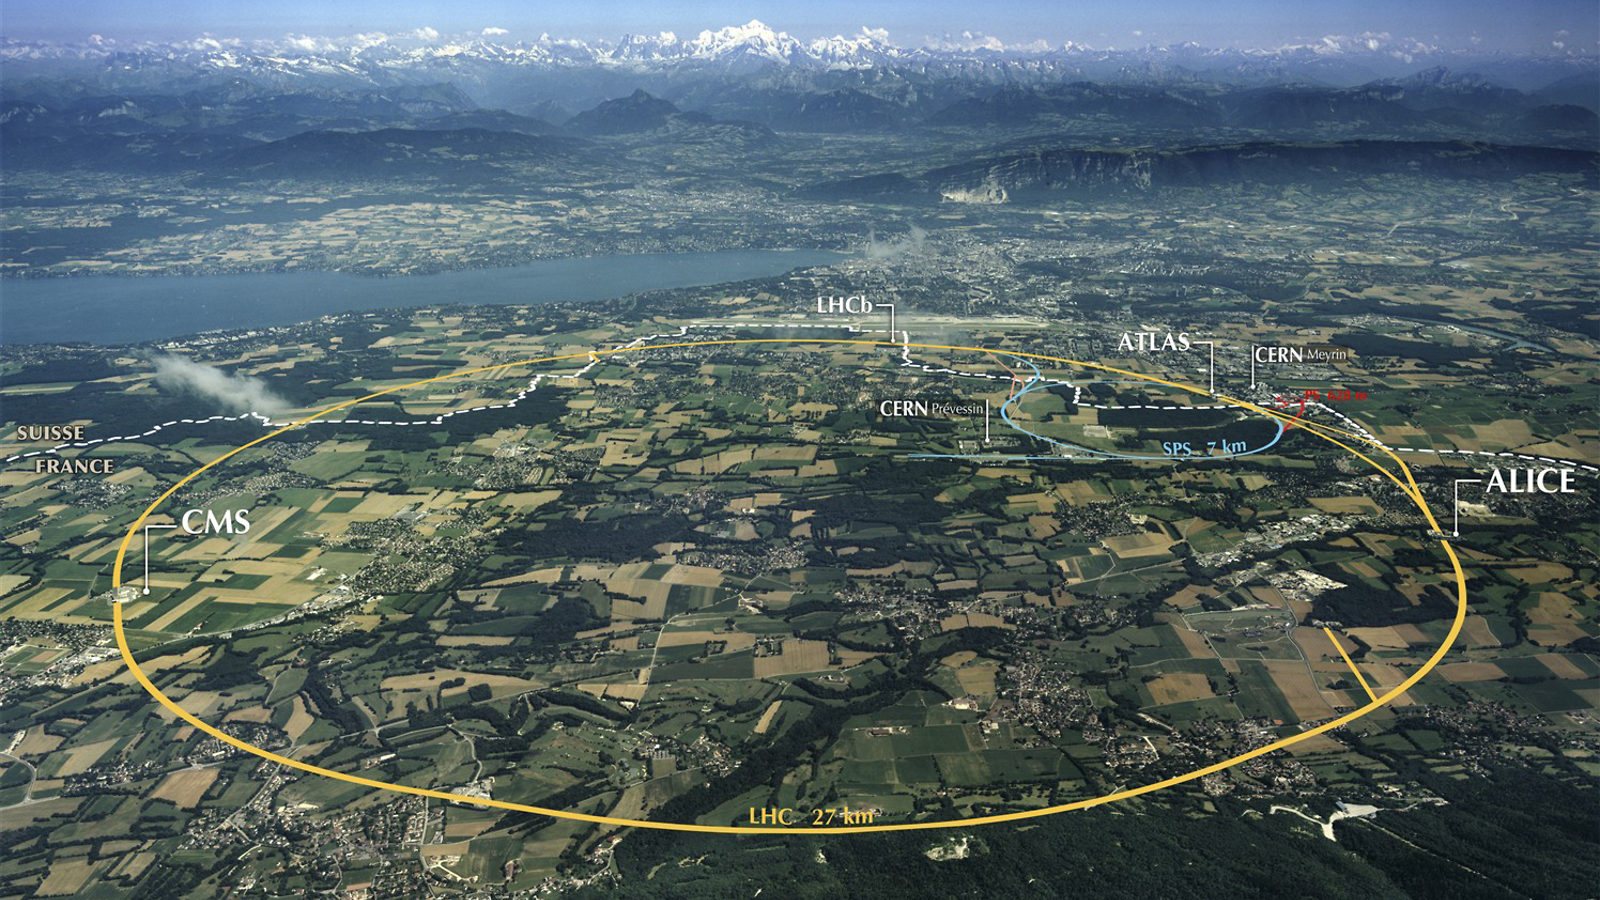
\includegraphics[width=\textwidth]{LHCearth}} \vfill
\caption{Disposición de los elementos principales del \lhc.} \label{fig_lhc}
\end{figure}

\vspace*{\fill}

\newpage


%%%%%%%%%%%%%%%%%%%%%%%%%%%%%%%%%%%%%%%%%%%%%%%%%%%%%%%%%%%%%%%%%%%%%%%%%%%%%%%%
\section{El CERN y su acelerador \lhc} %%%%%%%%%%%%%%%%%%%%%%%%%%%%%%%%%%%%%%%%%%%%%%%%%%%%%%%%%


El LHC es un acelerador circular de 27 km de longitud diseñado para producir colisiones $p-p$ a una energía máxima en el centro de masa de $\sqrt{s} = 14 \, \mathrm{TeV}$, permitiendo por tanto estudiar la escala de energías de $10^{12}$ eV y buscar nueva física. \color{vero} Desde 2008 opera en la misma obra civil que lo hacía LEP, \color{norm} soterrado a unos 150 metros de profundidad en la frontera franco-suiza, cerca de Ginebra como se ve en la Figura \ref{fig_lhcA}.

Los protones se extraen de fuentes de iones, como el duoplasmatrón, introduciendo gas hidrógeno,
y se van acelerando en una sucesión de  pre--aceleradores: LINAC, PSB, PS y  SPS, hasta finalmente llegar al LHC donde se alcanzan los $7 \, \mathrm{TeV}$ por haz (véase Figura \ref{fig_lhcA}).
%
Estos haces contienen $1.15 \times  10^{11}$ protones y se hacen cruzar con una frecuencia de $40$ MHz, dando el acelerador una luminosidad máxima de $10^{34} \, \mathrm{cm^{-2}s^{-1}}$.


A estas energías tan altas, para mantener a las dos corrientes de protones circulando a casi la velocidad de la luz y en órbitas contrarias, se necesitan fuertes campos magnéticos ($8.33 \, \mathrm{T}$ a $7 \, \mathrm{TeV}$), que se logran mediante potentes imanes superconductores refrigerados mediante helio super--fluido a  temperaturas de aproximadamente $1.9 \, \text{K}$. Para ello se  emplea un único crióstato con un flujo magnético circulando en sentido opuesto para cada corriente de protones.
 






La colisión de los dos haces tiene lugar en cuatro puntos  concretos del túnel, donde se hacen coincidir las trayectorias de ambos. 
Es en esos puntos dónde se sitúan los cuatro principales\footnote{Existen otros experimentos como TOTEM, que mide la secciones eficaces elásticas e inelásticas de las colisiones $pp$ ayudando al monitoreo de la luminosidad de CMS; o LHCf, que estudia a través los neutrones y fotones producidos a bajo ángulo en ATLAS los fenómenos de rayos cósmicos.} experimentos del LHC:

\begin{itemize}
 \item ALICE: Se dedica al estudio del Plasma de Quark y Gluones (\textit{Quark--Gluon Plasma}, QGP), un nuevo estado de agregación de la materia de extrema densidad y que se produce tras colisiones con iones pesados, para lo que se hacen circular iones Pb, en vez de protones.
 \item ATLAS: Creado para buscar el bosón de Higgs, es un detector de propósito general centrado en el estudio de los quarks t y b; diseñado para la detección de nuevas partículas pesadas en su capa de masa, buscando nueva física, así como evidencias de partículas de SUSY.
 \item CMS: Concebido para verificar de un modo distinto los resultados de ATLAS, es también un detector de propósito general con un programa de física similar.
 \item \lhcb: Es un detector especializado en medidas de precisión en violación CP, lo hace estudiando desintegraciones de los quarks b y c, teniendo como objetivo final entender mejor la asimetría bariónica del Universo, cuyo origen no se comprende en el \stdmod.
\end{itemize}

\color{vero}
Pueden verse representaciones de los cuatro detectores en la Figura \ref{fig_lhcdetect}. Cabe resaltar que el hito más grande, hasta la fecha, de ATLAS y CMS es el descubrimiento del bosón de Higgs en 2012; mientras que para \lhcb sus hitos son el descubrimiento de la desintegración ultra-rara $\Bs \rightarrow \muon \antimuon$, las medidas más precisas en las fases $\gamma$ y $\phis$, y el primer descubrimiento de estados de pentaquark.


\begin{figure}[H]
\subfloat[Detector ALICE \cite{alicedetector}.]{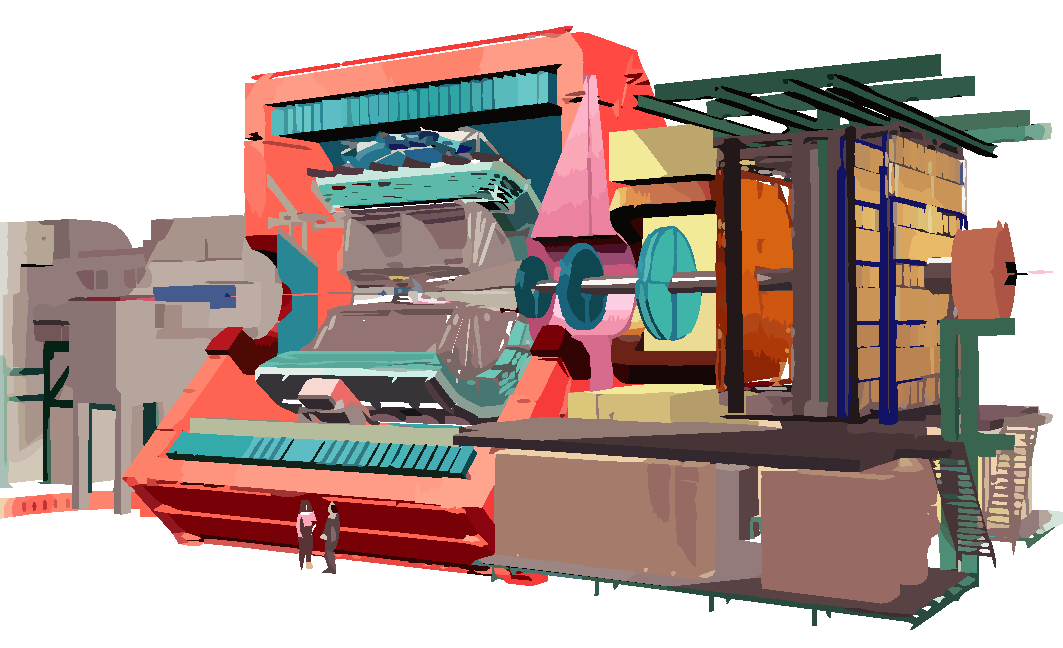
\includegraphics[width=0.48\textwidth]{ALICE.pdf}} \hfill
\subfloat[Detector ATLAS \cite{atlasdetector}.]{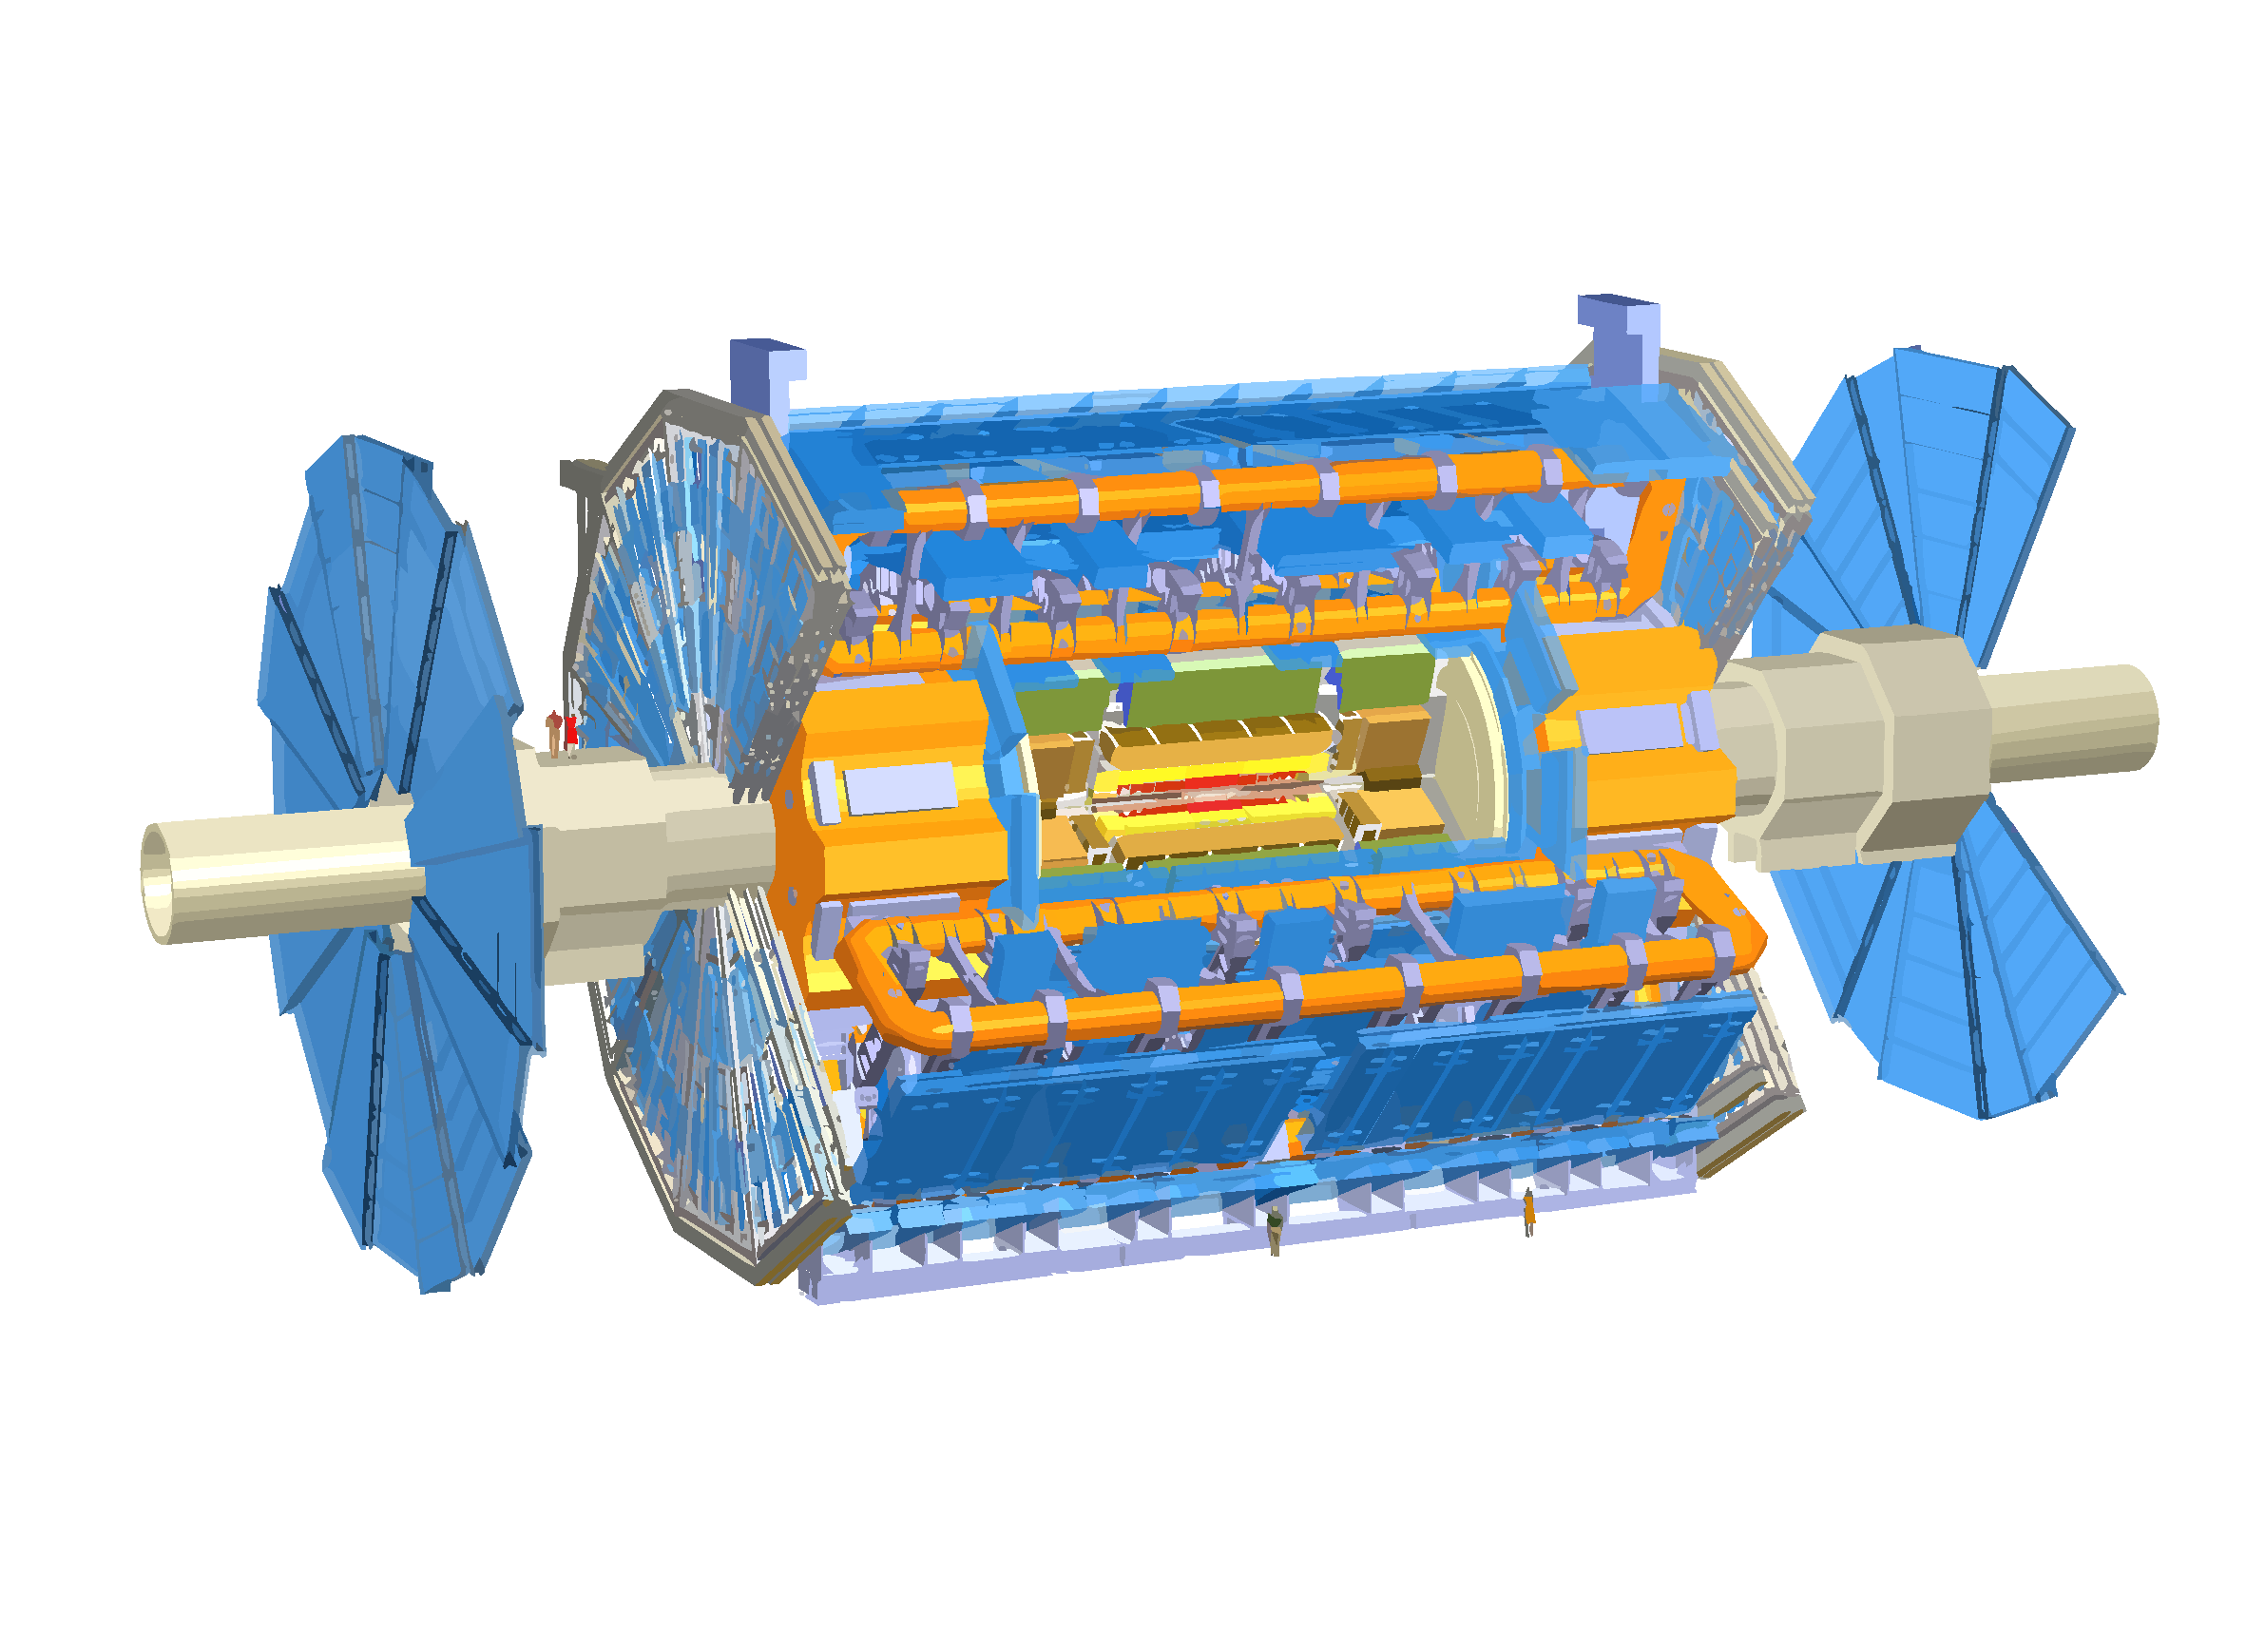
\includegraphics[width=0.48\textwidth]{ATLAS.pdf}} \hfill
%
\subfloat[Detector CMS \cite{cmsdetector}.]{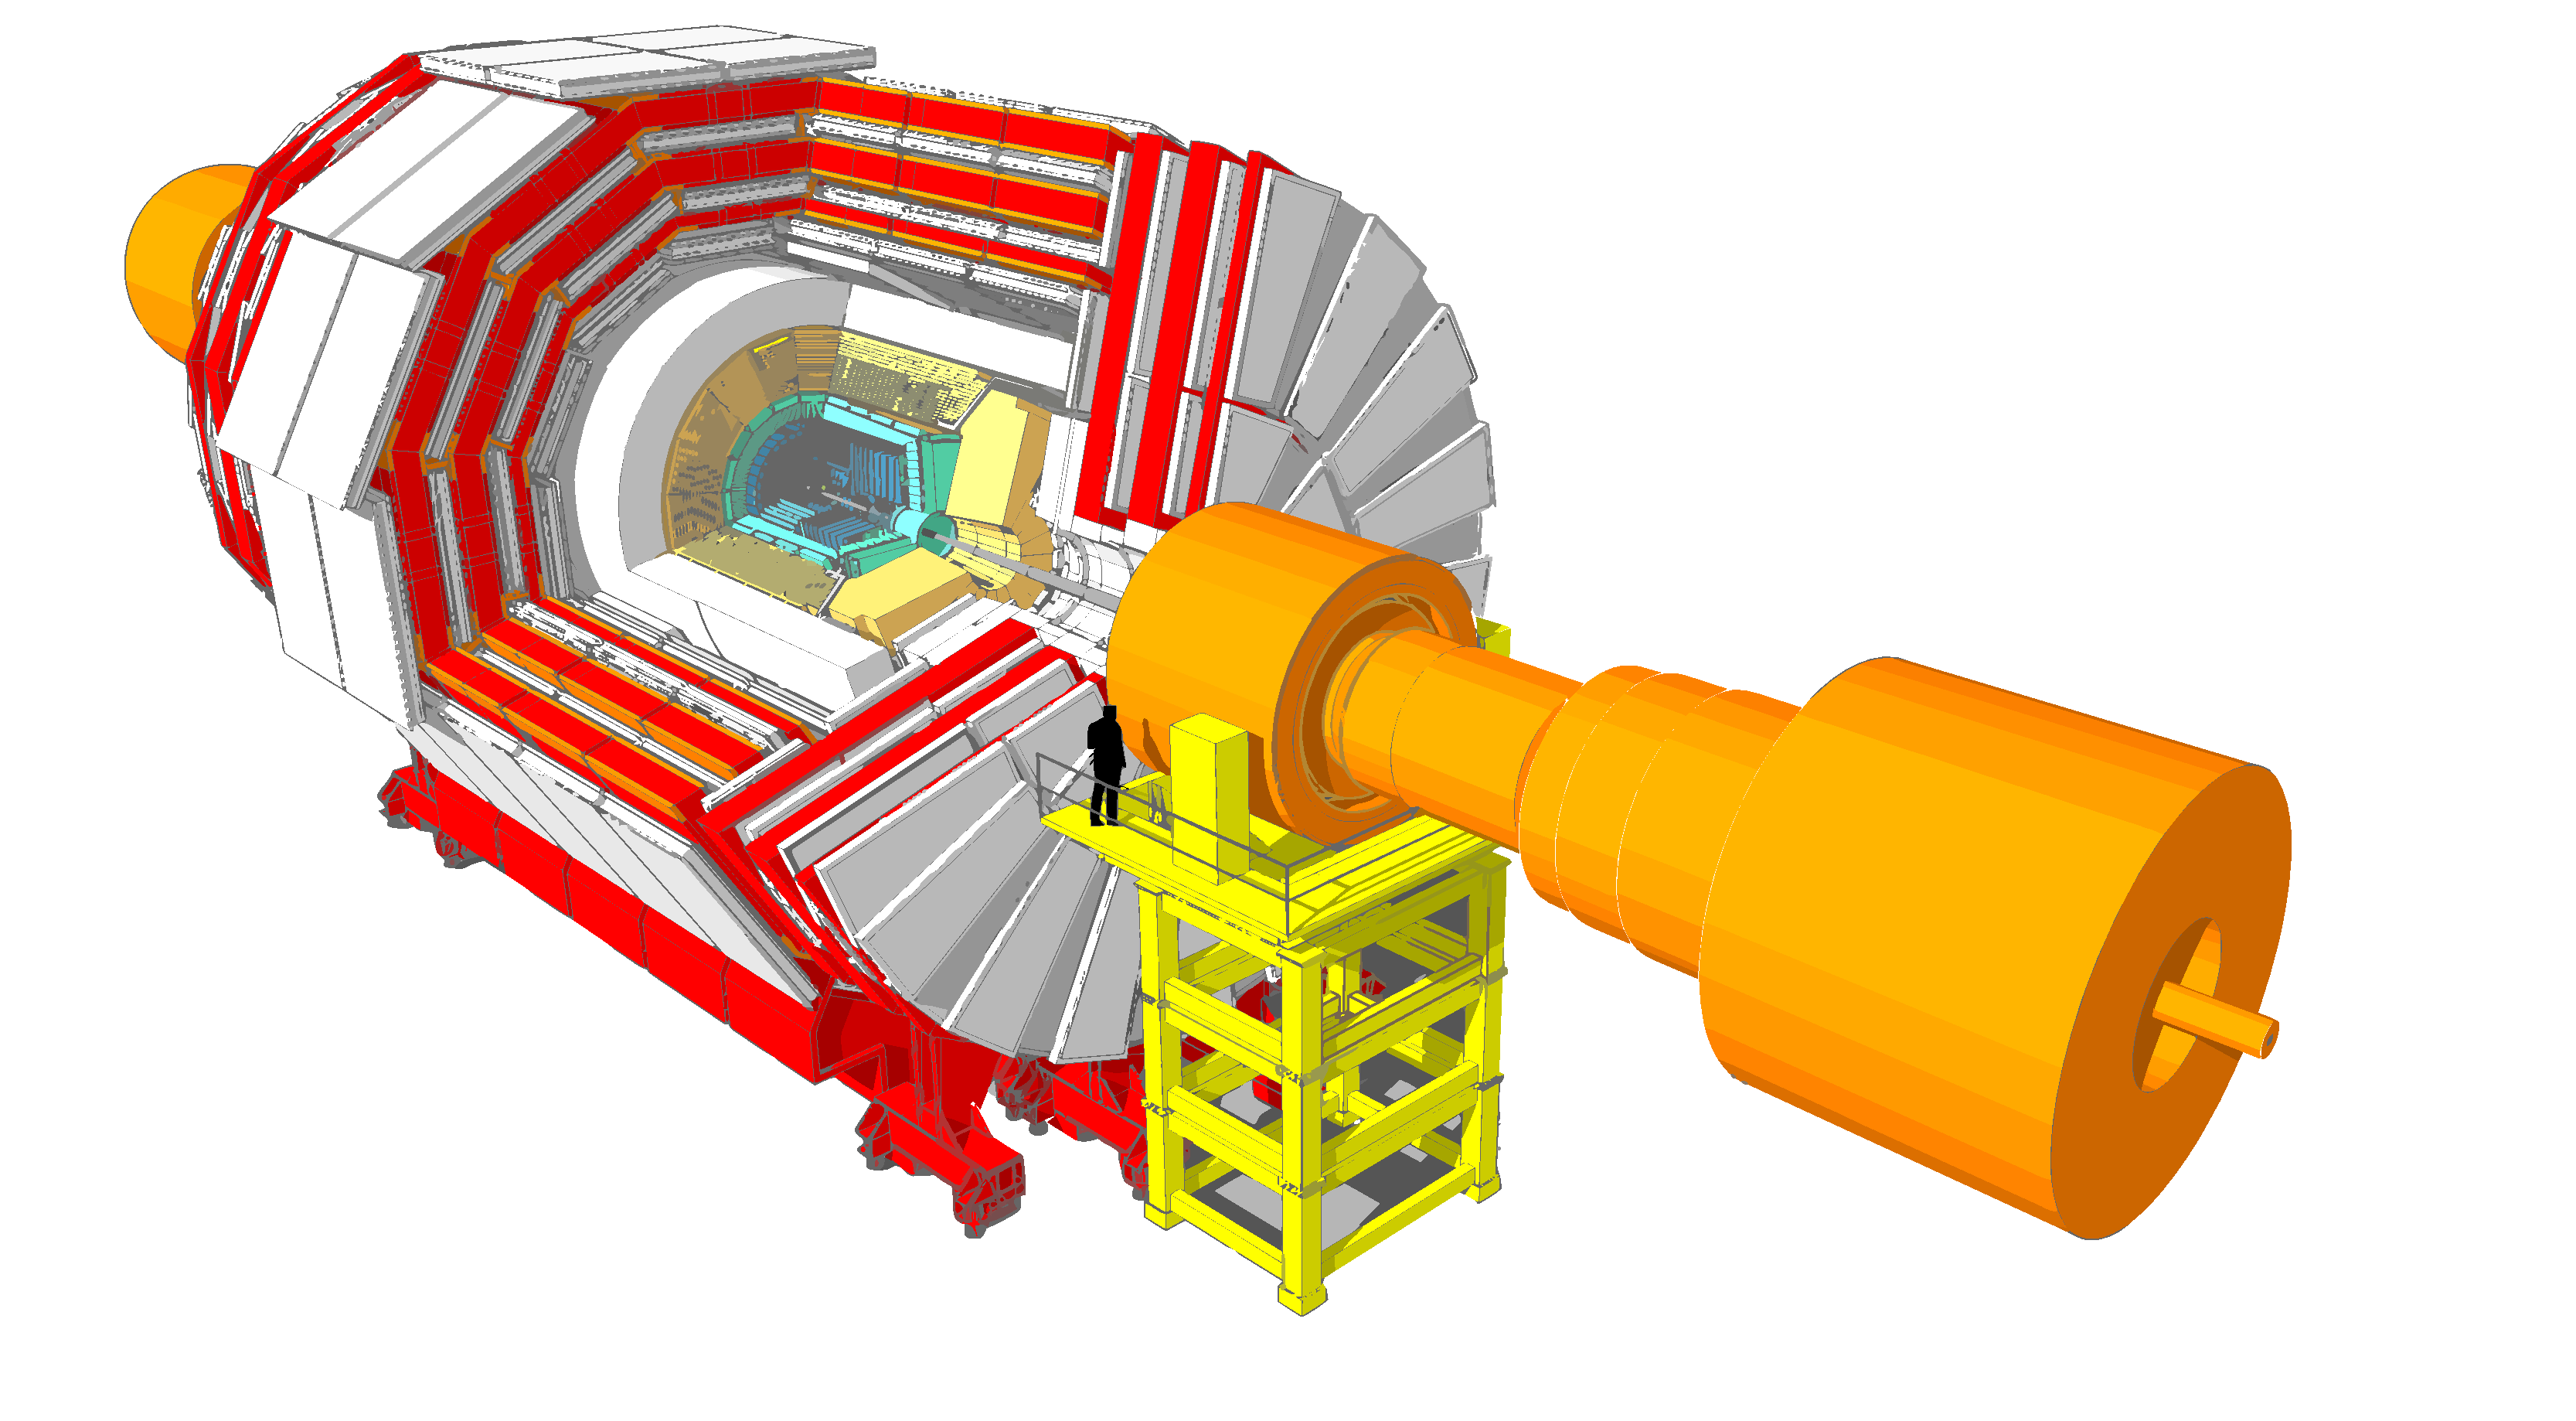
\includegraphics[width=0.48\textwidth]{CMS.pdf}} \hfill
\subfloat[Detector \lhcb \cite{lhcbdetector}.]{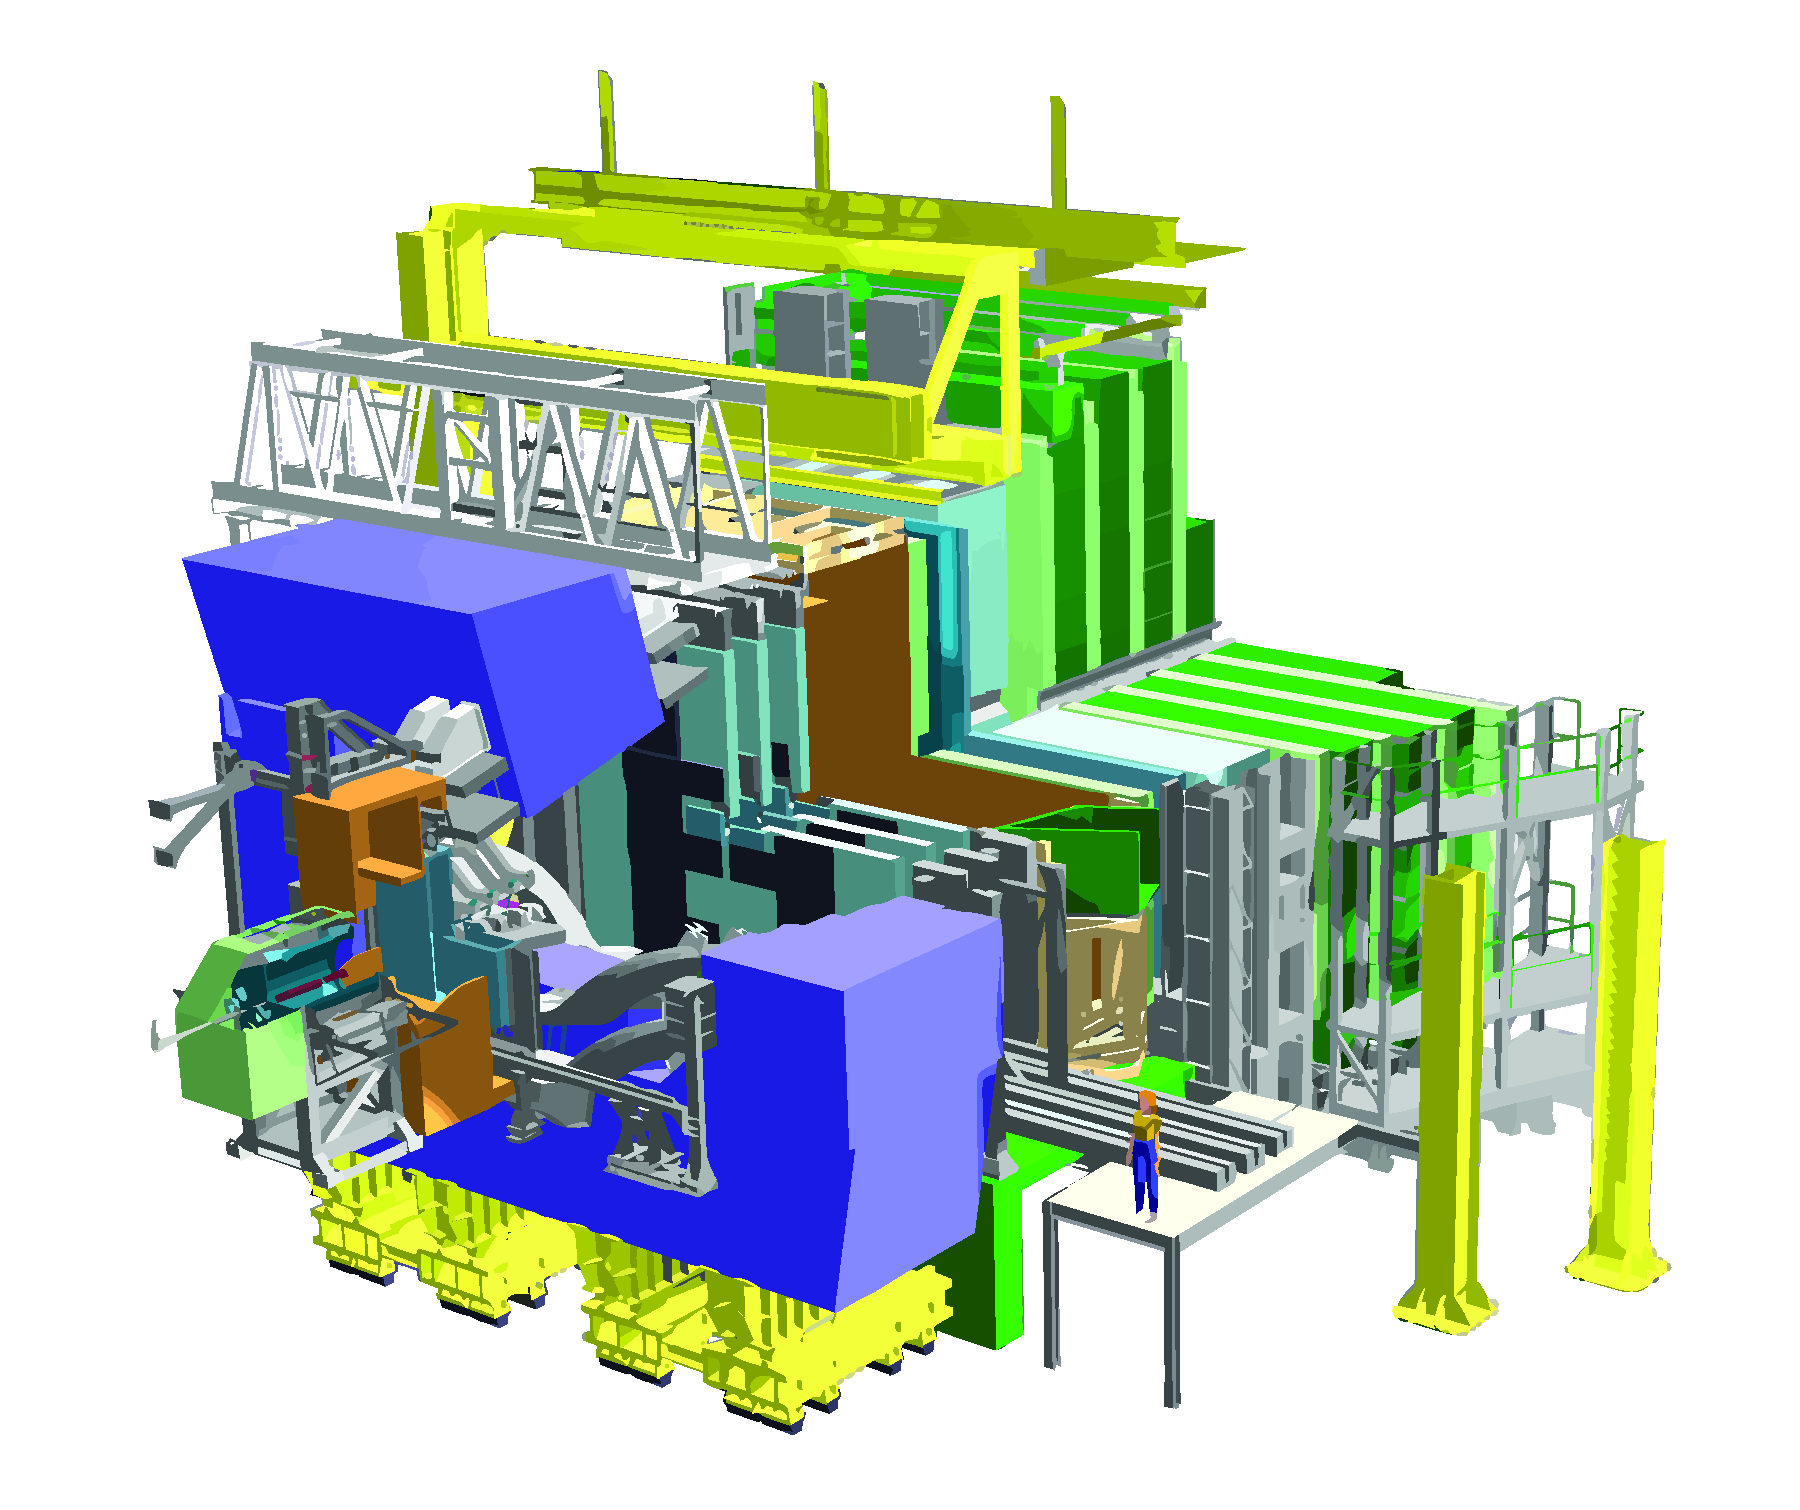
\includegraphics[width=0.48\textwidth]{LHCb.pdf}} \hfill
\caption{Esquemas (no en la misma escala) de los cuatro detectores principales de \lhc.} \label{fig_lhcdetect}
\end{figure}




%%%%%%%%%%%%%%%%%%%%%%%%%%%%%%%%%%%%%%%%%%%%%%%%%%%%%%%%%%%%%%%%%%%%%%%%%%%%%%%%
\section{El detector} %%%%%%%%%%%%%%%%%%%%%%%%%%%%%%%%%%%%%%%%%%%%%%%%%%%%%%%%%%

La idea original para la que \lhcb, Figura \ref{fig:partsLHCb}, fue diseñado era hacer estudios de precisión de los decaimientos raros de los quarks \emph{charm} y, sobre todo, \emph{bottom} \cite{Adeva:1224241,Alves:1129809}. El experimento, de $4500$ toneladas, situado en la antigua caverna de DELPHI (\textit{Detector with Lepton, Photon and Hadron Identication}, uno de los cuatro principales experimentos de LEP), fue diseñado específicamente para filtrar estas partículas. %La propia decisión de centrarse en los mesones B (aquellos formados por un quark b), provoca una constricción en el propio diseño del detector.  \color{norm}

\begin{figure}[H]
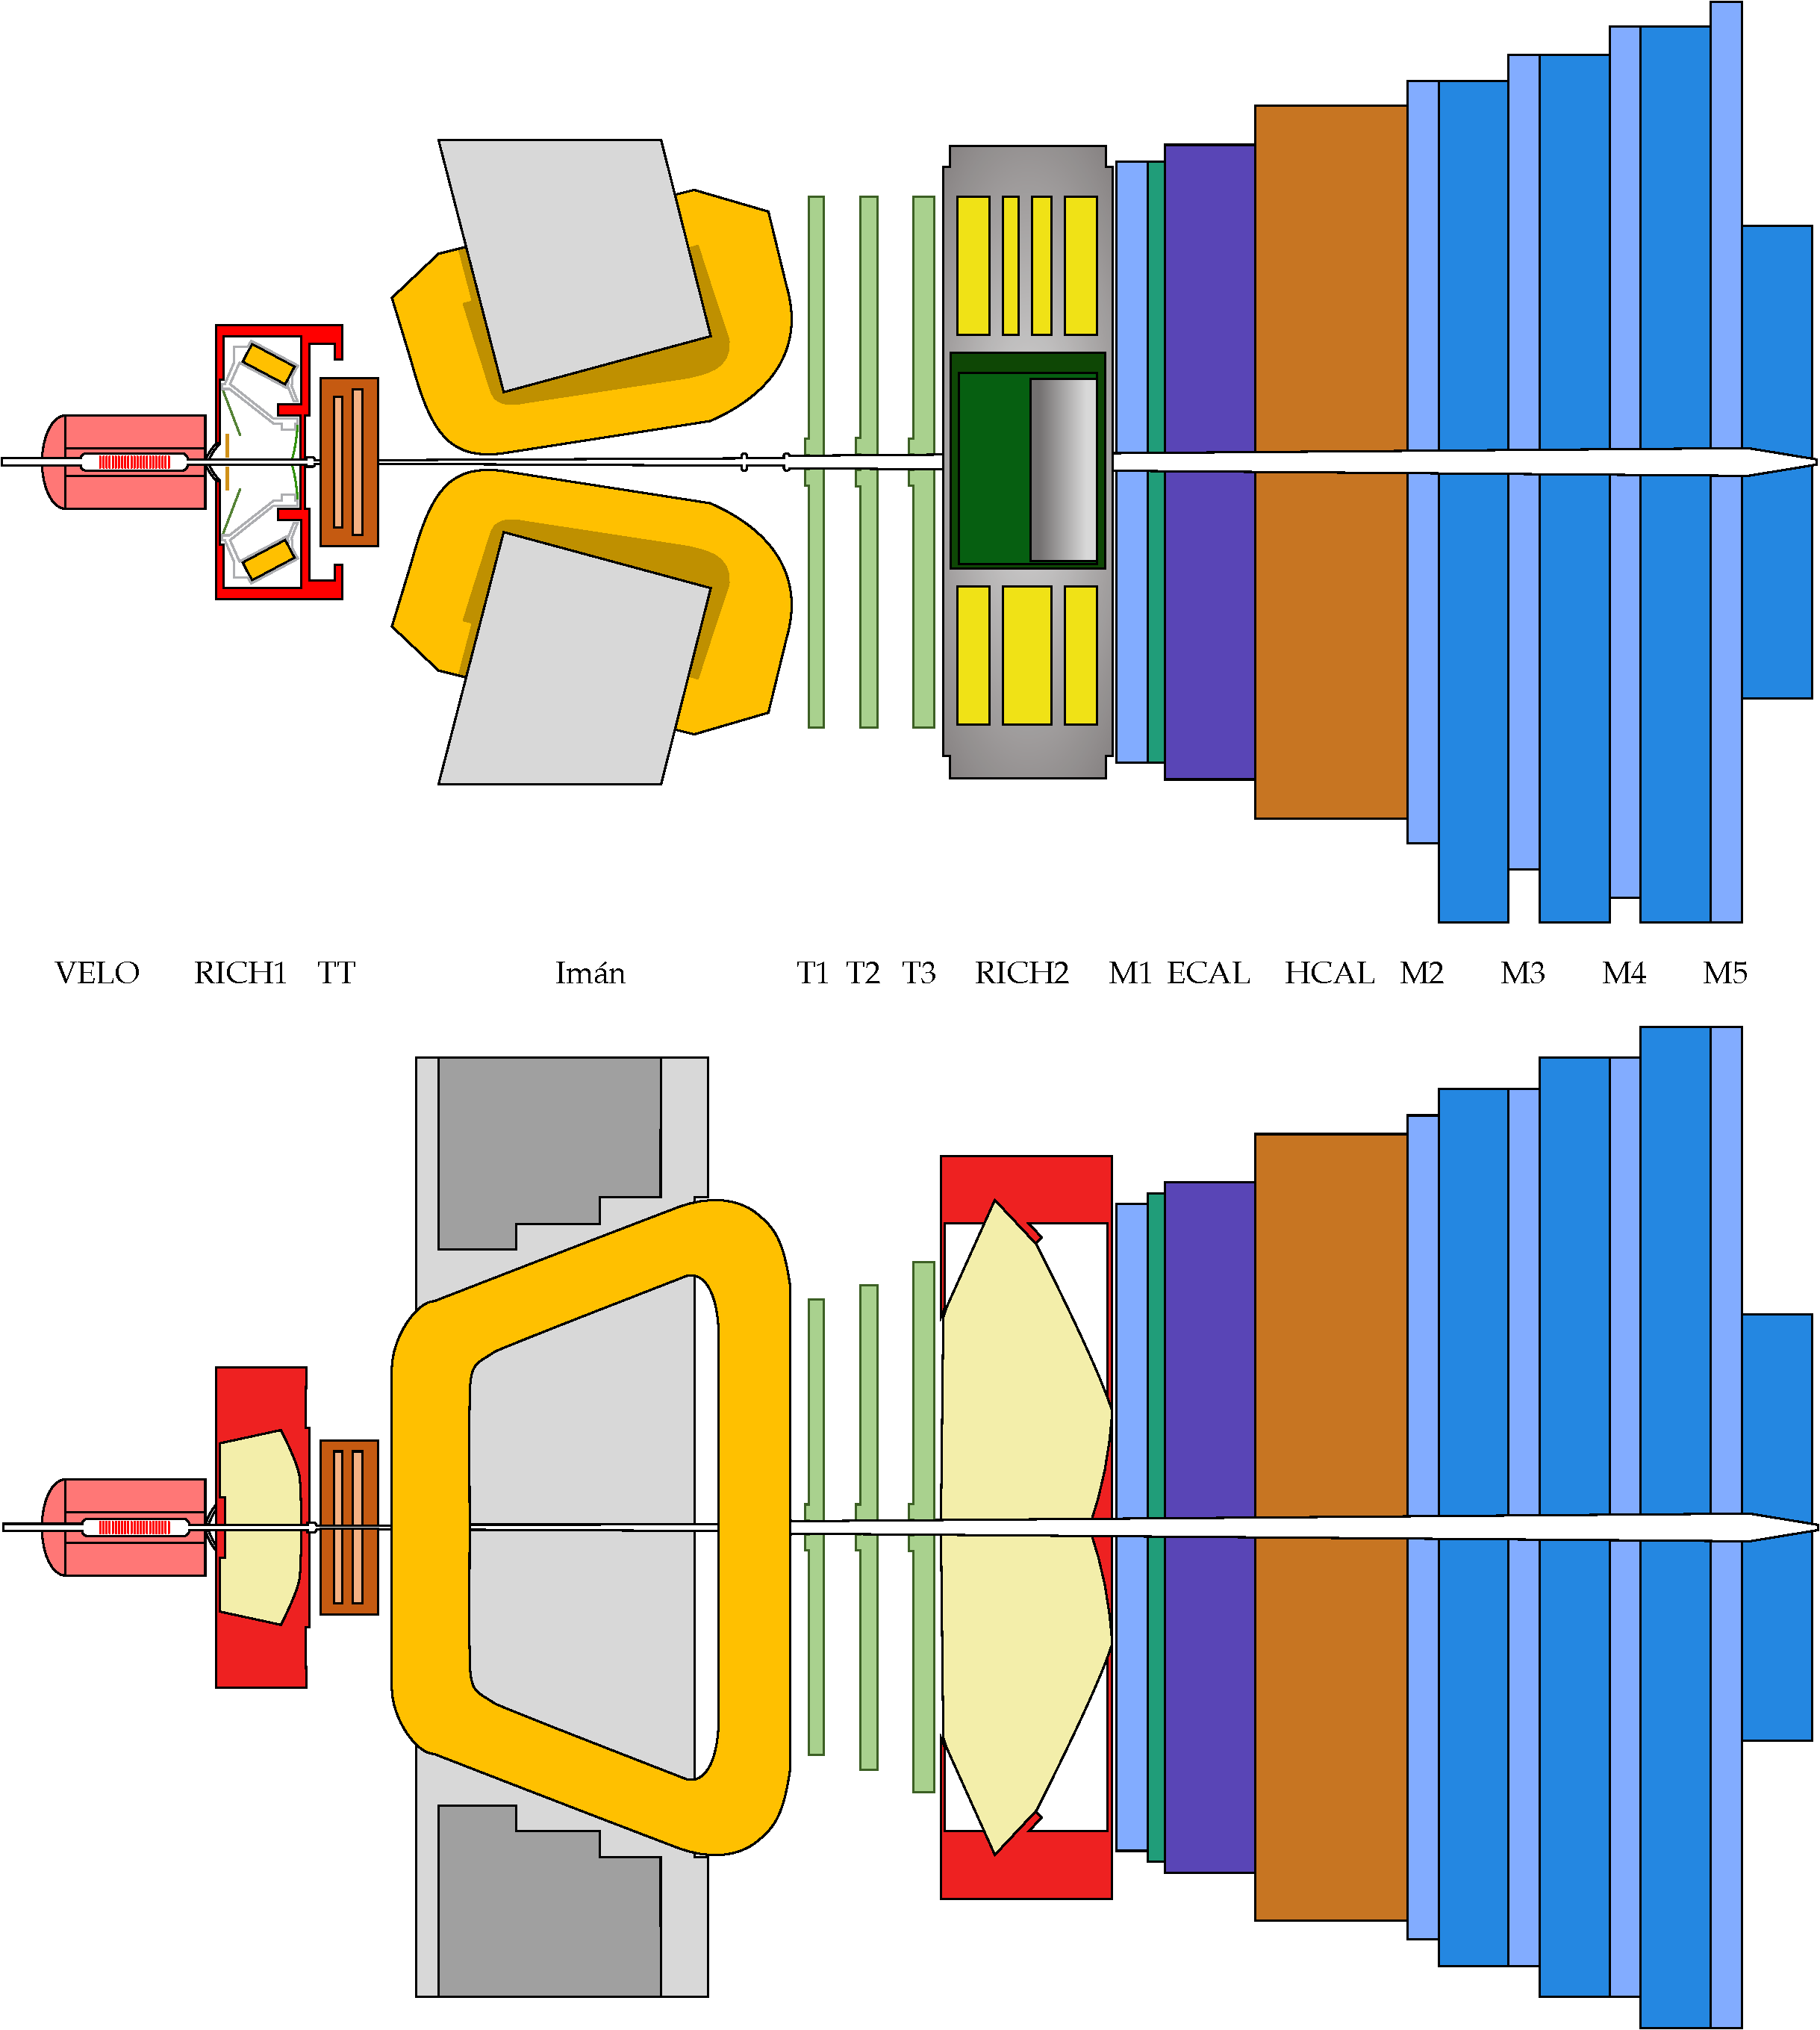
\includegraphics[width=\textwidth]{LHCbParts.pdf}
\caption{Detector \lhcb en dos vistas: arriba \textit{non-bending plane} (plano paralelo al campo magnético) y abajo \textit{bending plane} (plano perpendicular al campo magnético).}	\label{fig:partsLHCb}
\end{figure}

Dado que la sección eficaz de producción de pares $b$--$\bar b$ es muy alta para ángulos pequeños a estas energías 
%(ver figura <FIGURA>)
%  angle production figure
, \lhcb, a diferencia de los otros 3 detectores principales de LHC que tienen una estructura de barril y aceptancia quasi--$4 \pi$, es un detector de brazo único orientado en la dirección positiva \color{vero} de la circulación de los haces. \color{norm}
%
Así mismo, \lhcb se diseñó para trabajar a una luminosidad de entre $2$ y $5 \times 10^{32} \, \mathrm{cm^{-2}\, s^{-1}}$ \cite{Alves:1129809}, en vez de la nominal de \lhc $ 10^{34} \, \mathrm{cm^{-2}\, s^{-1}}$, de esta forma se puede asegurar una determinación precisa del vértice principal (PV) y del secundario (SV ---donde decaen las partículas) .

Su aceptancia varía desde los
 $10$ mrad hasta los $300$ mrad en el plano perpendicular al campo magnético ($250$ mrad en el paralelo) respecto al eje de los protones. Traduciendo estas cifras en pseudorapidez, $\eta$, \lhcb tiene una aceptancia que cubre el rango $2 < \eta < 5$ \cite{Alves:1129809}.

%TODO check footnote


%%%%%%%%%%%%%%%%%%%%%%%%%%%%%%%%%%%%%%%%%%%%%%%%%%%%%%%%%%%%%%%%%%%%%%%%%%%%%%%%
\subsection{Sistema de trazado} %%%%%%%%%%%%%%%%%%%%%%%%%%%%%%%%%%%%%%%%%%%%%%%%

A la hora de tomar los datos, \lhcb \cite{Alves:1129809} necesita tener una precisa determinación de las trayectorias en las que se desplazan las partículas.  Una vez que se reconstruye la traza, se puede determinar la carga de la partícula visto su comportamiento frente al imán, por ejemplo. Las combinaciones de varias trazas llevan a poder reconstruir vértices y medir con precisión su localización en el espacio. \lhcb cuenta con 3 sistemas de trazado: \color{vero} el \emph{Vertex Locator} (VELO), el \emph{Tracker Turicensis} (TT) y las estaciones de \emph{Tracking} 1, 2 y 3 (Tx). \color{norm}

\begin{figure}[H]
\includegraphics[width=\textwidth]{LHCbtracks}
\caption{Representación de los tipos de trazas, dependiendo de los volúmenes del espectrómetro que atraviesen.}	 \label{fig_tracks}
\end{figure}

\vspace*{-1cm}

La reconstrucción de eventos se fundamenta en determinar las trayectorias de todas las partículas cargadas y la posición en donde estas fueron generadas: los vértices. Para ello es preciso emplear, combinadamente, la información proporcionada por los tres sistemas de trazado. Dependiendo de la posición del vértice y de los \emph{hits},  se tienen las distintas posibilidades \color{vero} de la Figura \ref{fig_tracks}:\color{norm}
\begin{itemize}
	\item \textit{Long tracks}: Atraviesan todo el sistema de trazado, desde el VELO a las estaciones Tx y, dado que todos los detectores las miden, acaban siendo las medidas de momento más precisas, y las más importantes para \lhcb.
	\item \textit{Upstream tracks}: Atraviesan el VELO  y el TT; estos \emph{hits} se corresponden con partículas de poco momento y que el imán desvió fuera de la aceptancia del detector.
	\item \textit{Downstream tracks}: Atraviesan el TT y las estaciones Tx; estas trazas se corresponden con partículas de larga vida media que decaen fuera del VELO.
	\item \textit{VELO tracks}: Solo se miden en el detector homónimo y se corresponden con partículas que salen con un ángulo muy grande o hacia atrás, y que sirven principalmente en la reconstrucción del PV.
	\item \textit{T tracks}: Solo atraviesan las estaciones Tx; y corresponden a menudo con partículas generadas en interacciones secundarias.
\end{itemize}
%




\subsubsection{Vertex Locator}  %%%%%%%%%%%%%%%%%%%%%%%%%%%%%%%%%%%%%%%%%%%%%%%%

El Localizador de Vértice (VELO, \emph{\textsc{Ve}rtex \textsc{Lo}cator}) mide las posiciones espaciales de las trazas cerca del punto de colisión protón--protón, siendo así el primero de los detectores en entrar en acción. Esto permite separar el vértice principal (PV) del vértice secundario en donde estarían los hadrones con quarks $b$ o $c$.
Está conformado por $21 \times 2$ semidiscos ordenados, como se ve en la Figura \ref{fig_velo}, en la dirección del \textit{beam pipe}. Estos discos semicirculares están compuestos de micropistas de silicio y tienen en una cara los sensores $R$ (\emph{radial strips}) y en la opuesta los sensores $\phi$ (\emph{azimutal strips}), determinando así las coordenadas cilíndricas del PV. 

\vspace*{-0.5cm}

\begin{figure}[H]
\centering
\subfloat[Representación de los discos del VELO cerrado, para un \emph{beam} estable.\label{fig_velo_a1}]{\phantom{olaolaola}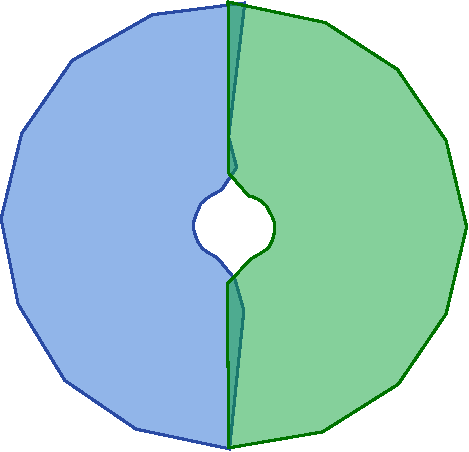
\includegraphics[height=0.2\textwidth]{VELOClosed.pdf} \phantom{olaolaola}} \hfill
\subfloat[Representación de los discos del VELO abierto, para la entrada de protones a \lhc.\label{fig_velo_a2}]{\phantom{olaol} 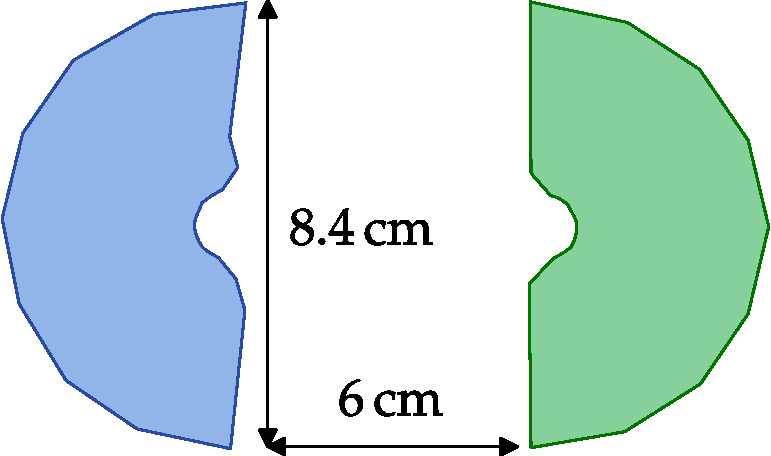
\includegraphics[height=0.2\textwidth]{VELOOpened.pdf} \phantom{olaol}}
 \\ 
 
\subfloat[Ubicación de los 42 semicírculos de micropistas de silicio que conforman el VELO. Se observa la alternancia entre detectores radiales y azimutales.\label{fig_velo_b}]{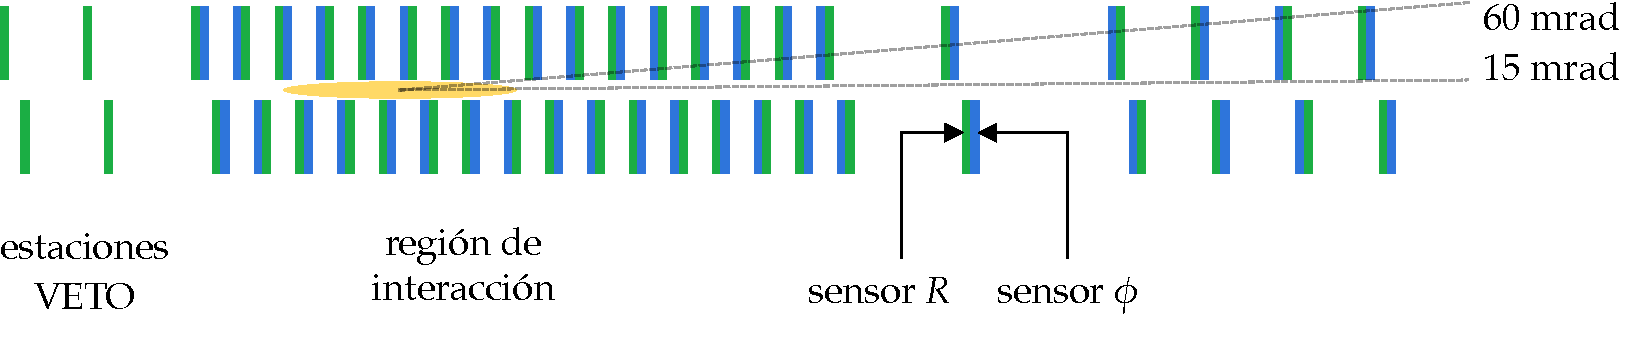
\includegraphics[width=\textwidth]{VELOStructure.pdf}} \hfill
\caption{Representación esquemática de partes del \emph{Vertex Locator}, detector donde se determina el PV y SV.} \label{fig_velo}
\end{figure}


Para tener la mejor precisión posible en la resolución del PV, la medida de la traza convendría que se realizase lo más cerca posible de la interacción. El VELO tiene área sensible desde tan solo $8$ mm del \emph{beam pipe}, demasiado pequeña para el proceso de inyección de protones al LHC. Cuando se están introduciendo protones en el tubo principal, o mientras hay inestabilidades en el haz, el VELO se puede separar $3$ cm del tubo, protegiendo así al detector de la radiación. El VELO es capaz de determinar las longitudes de decaimiento del B y D con una precisión de entre $220$ y $375 \,\upmu$m, y localizar el PV con una precisión de hasta $10 \, \upmu$m en el plano perpendicular y hasta $42 \,\upmu$m en la dirección del haz.
 
La aceptancia del VELO cubre $1.6<\eta<4.9$ para las partículas en el PV. Al principio del VELO (véase Figura \ref{fig_velo_a2}) se observan 2 capas de pistas tipo R, que constituyen el \emph{pile--up VETO system}, que desecha los eventos que cuentan con un número grande de vértices primarios (\emph{high multiplicity events}) de esto se informa el \texttt{L0--trigger} descrito en \S \ref{sec_l0trigger}. 





\subsubsection{Tracking Turicensis y estaciones de trazado} %%%%%%%%%%%%%%%%%%%%

Tanto a la entrada como a la salida se colocan detectores de trazas, para ver cómo afecta el imán a sus trayectorias. El TT junto con las estaciones Tx son los principales detectores a la hora de medir el momento de las trazas en \lhcb \cite{Alves:1129809}. Tenemos dos tipos de detectores aquí: los detectores de micropistas de silicio y las cámaras de deriva.

\begin{description}

	\item[Silicon Tracker] \color{vero} Se denomina Silicon Tracker (ST) al conjunto formado por el TT y la parte más cercana al \emph{beam pipe} de las estaciones Tx, el Inner Tracker (IT); ambos ellos empleando la tecnología de silicio, cuyos detectores aparecen en la Figura \ref{fig_sillicontracker1}. \color{norm}
	El ST está compuesto por cuatro capas de detectores: dos verticales (la primera y última) y dos que se encuentran giradas por $\pm 5\,{}^{\circ}$ en medio de las anteriores. La separación entre las pistas es de $20\, \mathrm{\upmu m}$, lo que se traduce \color{vero} en \color{norm} una resolución de $50\,\mathrm{\upmu m}$. El TT está diseñado para cubrir el rango de aceptancia del detector, mientras que el ST se encuentra principalmente alrededor del \emph{beam pipe} y solo constituye el $1.3 \, \%$ de las estaciones de trazado.
\begin{figure}[H]
\centering
\subfloat[Representación del \emph{Tracker Turicensis}.\label{fig_st_a}]{\phantom{olaola}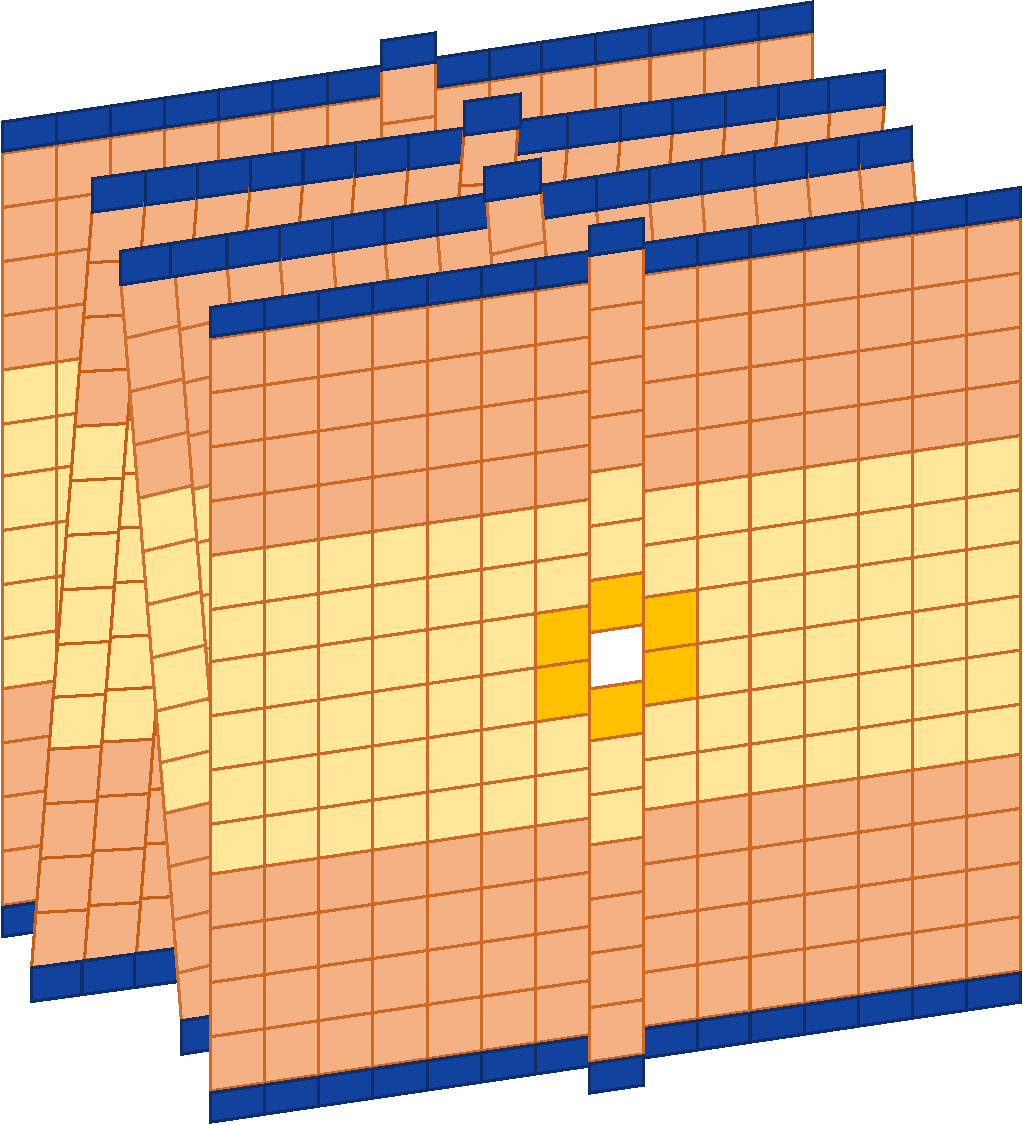
\includegraphics[width=0.3\textwidth]{TT.pdf}\phantom{olaola}} \hfill 
\subfloat[Representación de un \emph{Inner Tracker} de una estación Tx.\label{fig_st_b}]{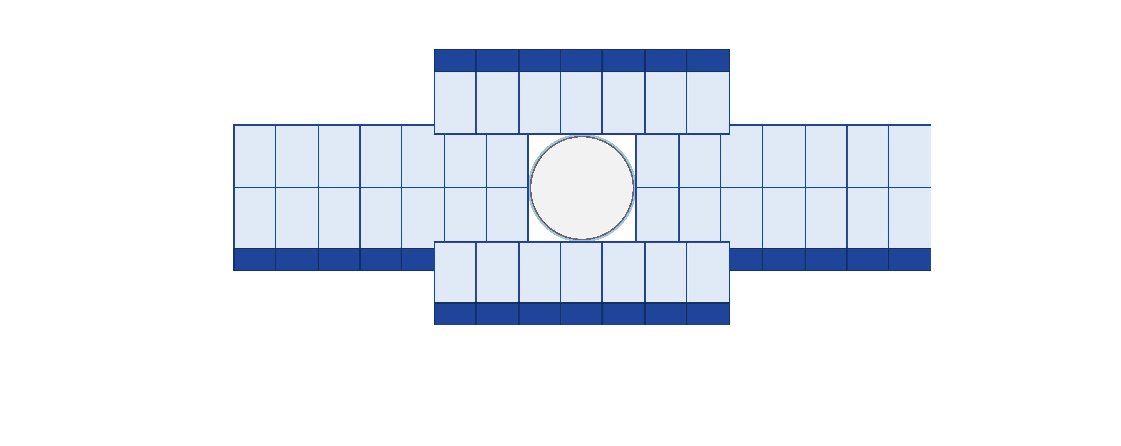
\includegraphics[width=0.5\textwidth]{IT.pdf}} \hfill
\caption{Elementos del \emph{Silicon Tracker}, las estaciones de trazado que emplean tecnología de silicio.} \label{fig_sillicontracker1}
\end{figure}

	\item[Outer Tracker]  Las \color{vero}estaciones Tx, representadas en la Figura \ref{fig_sillicontracker2}, \color{norm} se conforman en su parte más externa del OT, un detector de cámaras de deriva que tiene una resolución en la traza de $200\, \mathrm{\upmu m}$ y que emplea una mezcla 70--30 de argon y $\mathrm{CO_2}$ como gas. Los módulos del OT se organizan en tres estaciones de trazado, cada una de ellas con cuatro capas de detección que siguen el mismo patrón que las descritas para el ST.
\begin{figure}[H]
\centering
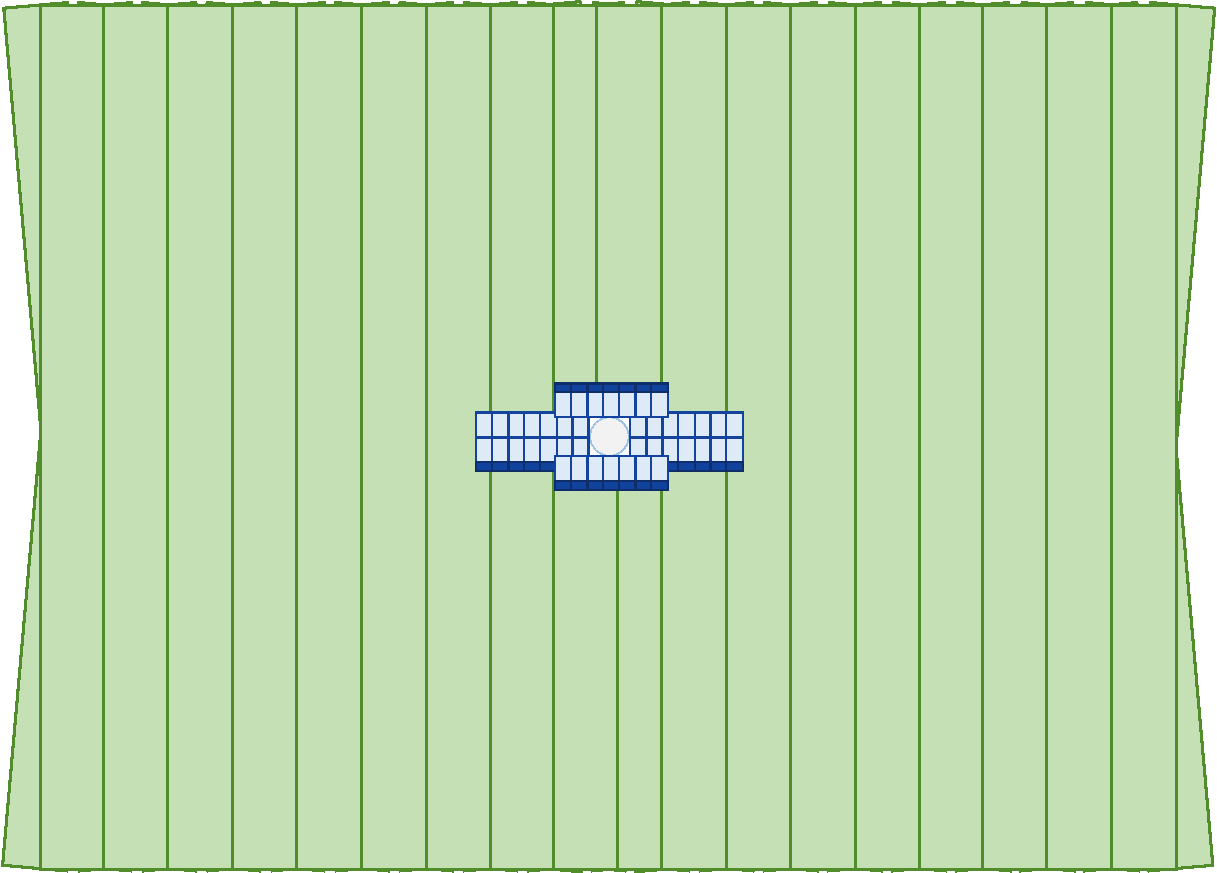
\includegraphics[width=0.48\textwidth]{OT.pdf}
\caption{Representación de las estaciones Tx, donde puede verse en verde el \emph{Outer Tracker}.} \label{fig_sillicontracker2}
\end{figure}

\end{description} 



%%%%%%%%%%%%%%%%%%%%%%%%%%%%%%%%%%%%%%%%%%%%%%%%%%%%%%%%%%%%%%%%%%%%%%%%%%%%%%%%
\subsubsection{Imán} %%%%%%%%%%%%%%%%%%%%%%%%%%%%%%%%%%%%%%%%%%%%%%%%%%%

%TODO <FIGURE> of magnet
Se trata de un imán dipolar de bobinas convencional de $4 \, \mathrm{T\,m}$ de inducción magnética integrada a temperatura ambiente. Las bobinas, con forma de silla cónica y situadas simétricamente, están fabricadas en Al--99.7, puro que rodea a un núcleo de hierro; pesando cada una de ellas 27 toneladas \cite{Alves:1129809}.

Las partículas cargadas se curvan al atravesar el campo magnético, permitiendo así medir su momento. La diferencia entre el gradiente de las trazas en el VELO y en las estaciones Tx es inversamente proporcional al momento de la partícula. 
Destacar que, para la reducción de uncertidumbres sistemáticas a causa de diferencias en la detección de partículas con cargas distintas, \color{norm} se cambia periódicamente la dirección del campo magnético.



%%%%%%%%%%%%%%%%%%%%%%%%%%%%%%%%%%%%%%%%%%%%%%%%%%%%%%%%%%%%%%%%%%%%%%%%%%%%%%%%
\subsection{Identificación de partículas en los detectores} %%%%%%%%%%%%%%%%%%%%

La identificación de partículas es clave en \lhcb por varias razones, entre las que destacan: el permitir identificar el sabor (\emph{flavour}) de los mesones B y la posibilidad de eliminar \color{vero} fondos \color{norm} que son similares a la señal. En \lhcb hay tres tipos de detectores: RICH, calorímetros y detectores de muones.

%\begin{figure}[H]
%\includegraphics[scale=0.48]{lhcbpid}
%\caption{Representación de los detectores involucrados en la identificación de partículas. <maybe remove this one>}	
%\end{figure}



\subsubsection{Detectores RICH} %%%%%%%%%%%%%%%%%%%%%%%%%%%%%%%%%%%%%%%%%%%%%%%%

Estos detectores tienen como principio de funcionamiento la radiación Cherenkov emitida por partículas relativistas cargadas que atraviesan un medio con una velocidad superior a la de la luz ($c$) en ese medio. Entonces, midiendo $\cos \theta_C = \sfrac{c}{vn}$ ($n$ es el índice de refracción del medio) y combinándola con el momento, se puede inferir la masa y por tanto el tipo de partícula.

En \lhcb hay dos detectores RICH \cite{Alves:1129809}, uno a la entrada y otro a la salida del imán dipolar. El RICH1, situado antes del imán, emplea aerogel y $\mathrm{C_4F_{10}}$ como radiadores y está optimizado para partículas de bajo momento, $1-60 \, \mathrm{GeV\, c^{-1}}$. EL RICH2, situado después de las estaciones de trazado Tx, emplea $\mathrm{CF_4}$ como radiador y detecta partículas con momento $15-100 \, \mathrm{GeV\, c^{-1}}$. Pueden verse representaciones de ambos detectores en la Figura \ref{fig_richdectectors}.
%
La aceptancia del RICH1 es de $250$ mrad, mientras que la del RICH2 es de $120$ mrad. En ambos, la luz Cherenkov que se produce al atravesar las partículas del material radiador se refleja en combinaciones de espejos planos y esféricos conduciéndola fuera de la aceptancia del detector donde es captada por \textit{Hybrid Photon Detectors} (HPD).

La misión fundamental del RICH es la identificación de partículas cargadas, nombradamente: $\uppi$, K y p.  Los anillos Cherenkov que se producen se identifican en los HPD  y se comparan con ciertas distribuciones para diferentes hipótesis en las trazas. Se define una \emph{likelihood} para todas las trazas y se minimiza para la hipótesis de partículas.

\begin{figure}[H]
\centering
\subfloat[Representación de la vista lateral del RICH1.\label{fig_rich1}]{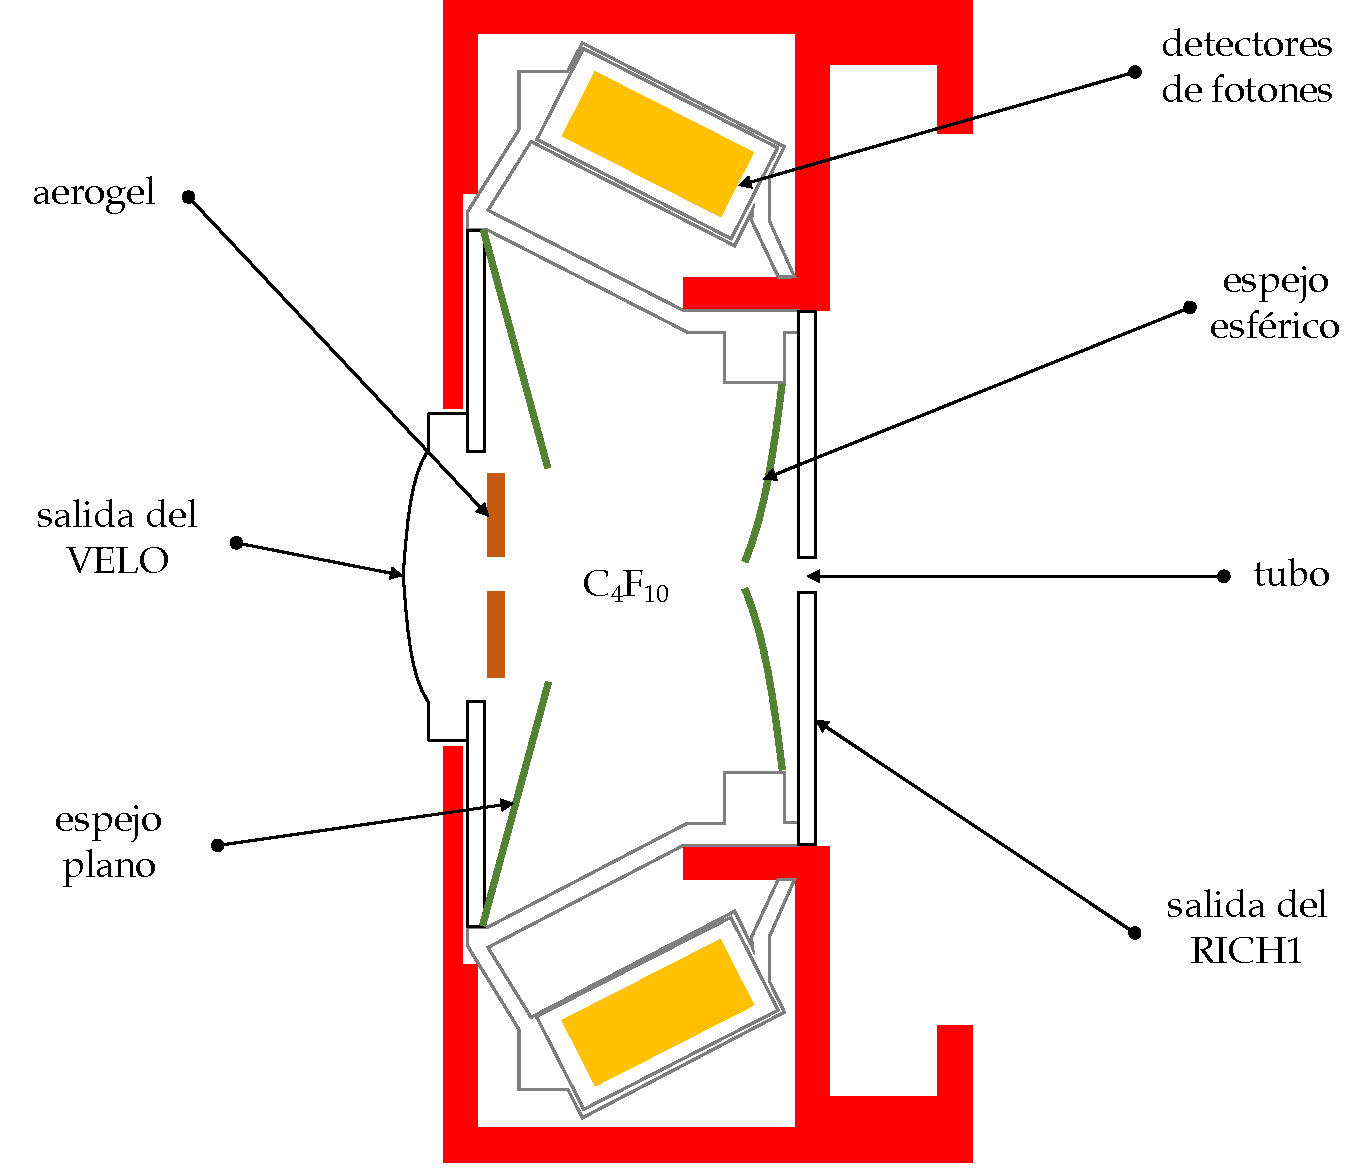
\includegraphics[height=0.4\textwidth]{RICH1}} \hfill
\subfloat[Representación de la vista desde arriba del RICH2.\label{fig_rich2}]{\phantom{olaola}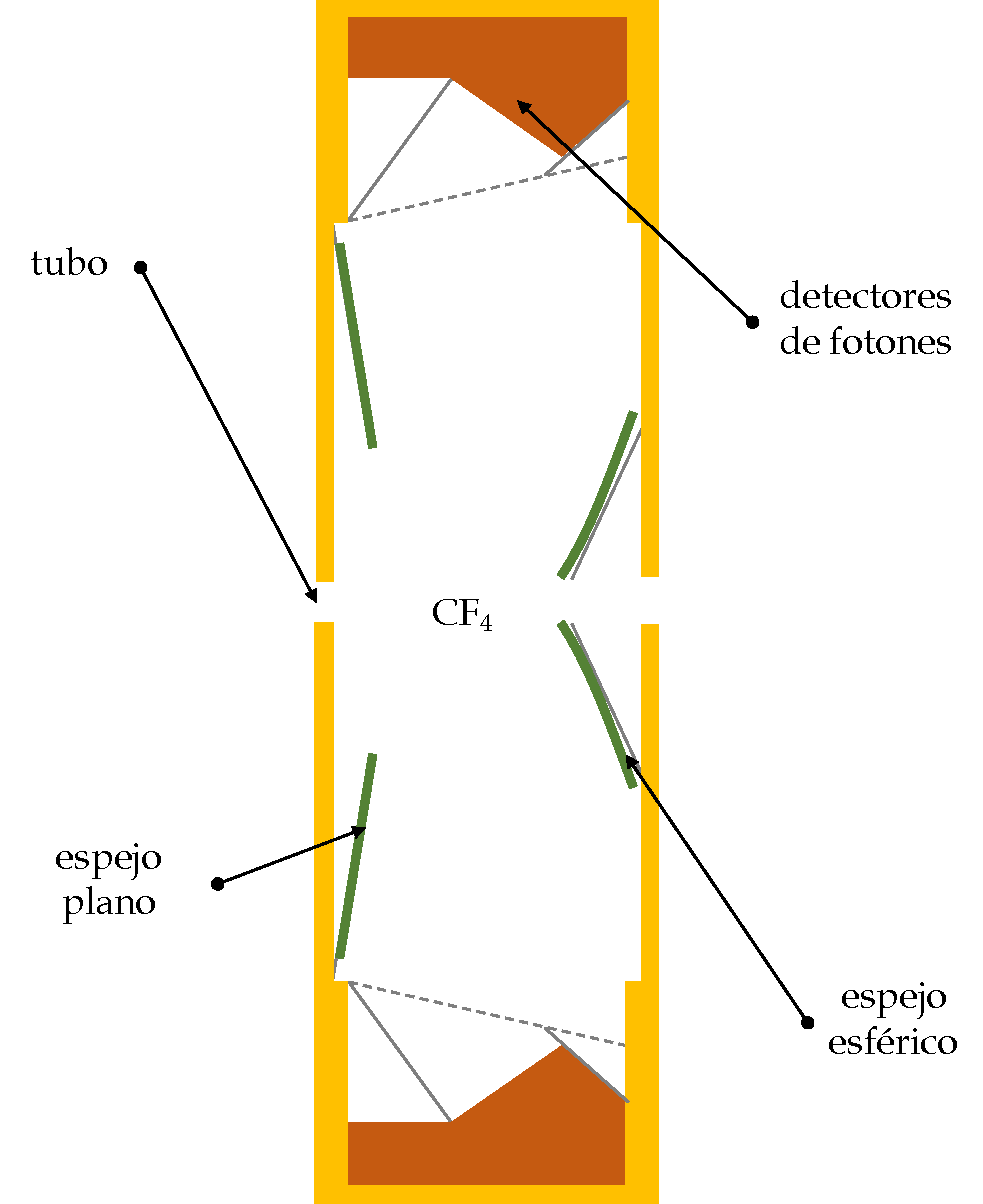
\includegraphics[height=0.4\textwidth]{RICH2}\phantom{olaola}} \hfill
\caption{Representación de los detectores RICH y de sus partes principales.} \label{fig_richdectectors}
\end{figure}



\subsubsection{Calorímetros} %%%%%%%%%%%%%%%%%%%%%%%%%%%%%%%%%%%%%%%%%%%%%%%%%%%

El sistema de calorímetros tiene como principal función determinar la energía \color{vero} transversal, \color{norm} $E_T$, que necesita el \texttt{L0}--\emph{trigger}, midiéndola a partir de la que depositan las partículas en las capas de material absorbente. 
Además, con la configuración de calorímetros de \lhcb, se pueden identificar también las partículas, una vez estas depositan toda su energía cinética dando lugar a cascadas de partículas que son caracterizadas por los calorímetros. Todos los calorímetros se encuentran divididos en celdas, permitiendo así medir la posición de la energía que se va depositando en las diferentes celdas.

%\begingroup
%\mySfFamily
%This should be sans-serif : $dfgd, \Q, \N, \Z, \C$ are sets.
%\endgroup


El sistema de calorímetros de \lhcb \cite{Alves:1129809} se compone de cuatro elementos, ordenadamente: \emph{Scintillating Pad Detector} (SPD), que detecta si las partículas entrantes son neutras o tienen carga; \emph{Preshower} (PS), que distingue entre electrones y hadrones cargados, y fotones de hadrones neutros, gracias a una lámina de plomo que se ubica entre el SPD y este mismo; \emph{Electromagnetic Calorimeter} (ECAL), que alterna centelleadores y láminas de plomo para identificar partículas no hadrónicas y tiene un espesor de 25 longitudes de radiación; \emph{Hadronic Calorimeter} (HCAL), que alternando material centelleador con láminas de hierro y con un espesor de 6 longitudes de interacción nuclear, identifica los hadrones.

\begin{figure}[H]
\centering
\subfloat[Representación de las celdas de un cuarto del ECAL.\label{fig_ecal}]{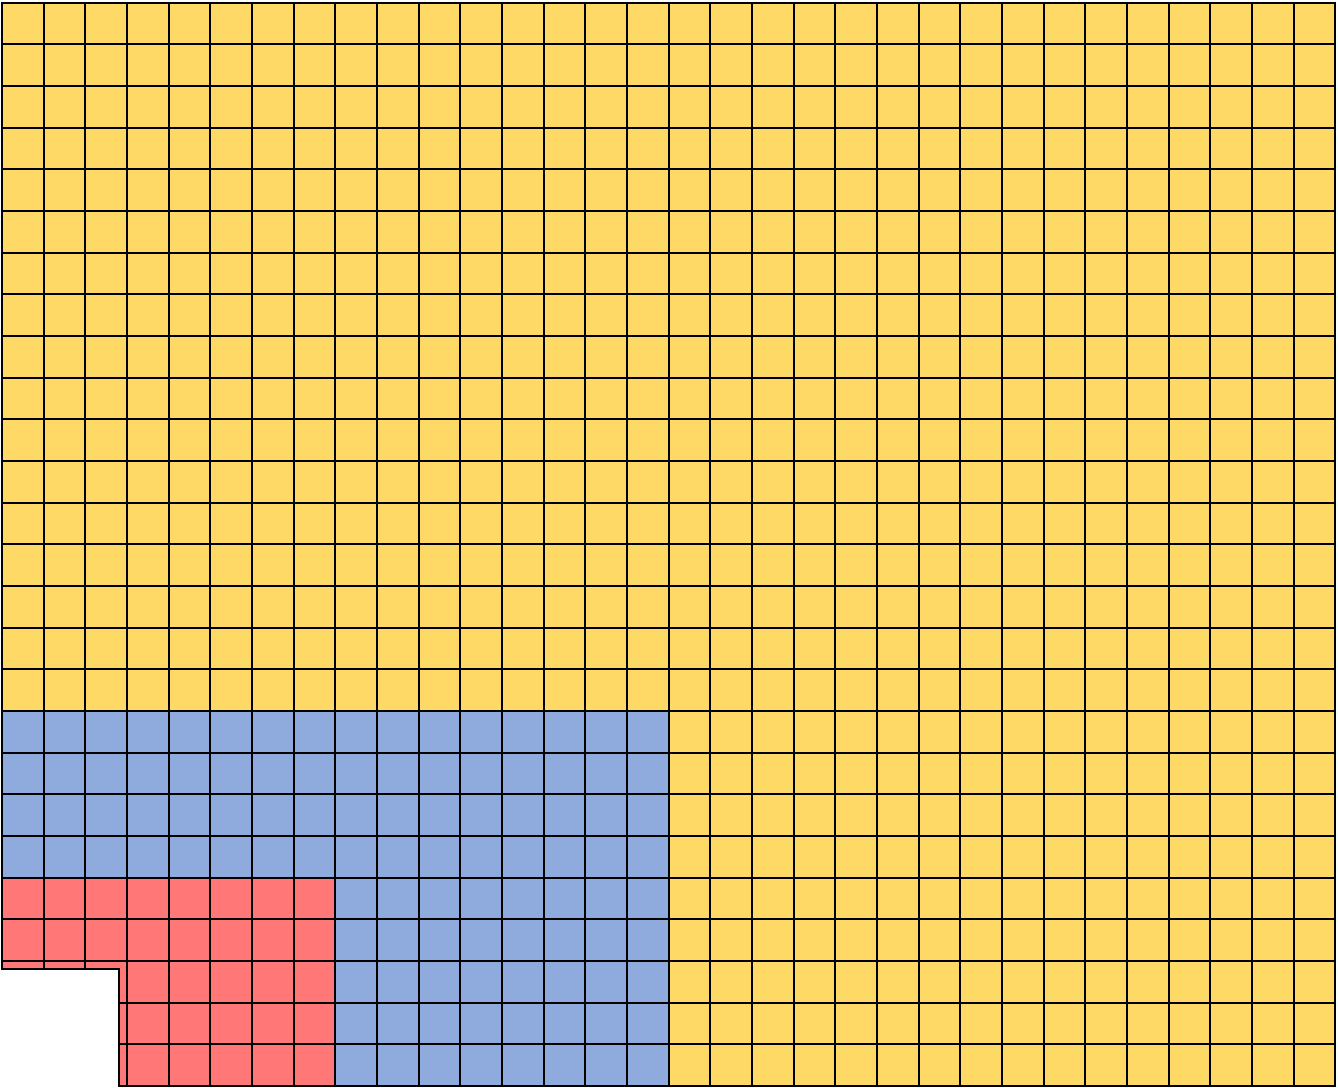
\includegraphics[width=0.48\textwidth]{ECAL}} \hfill
\subfloat[Representación de las celdas de un cuarto del HCAL.\label{fig_hcal}]{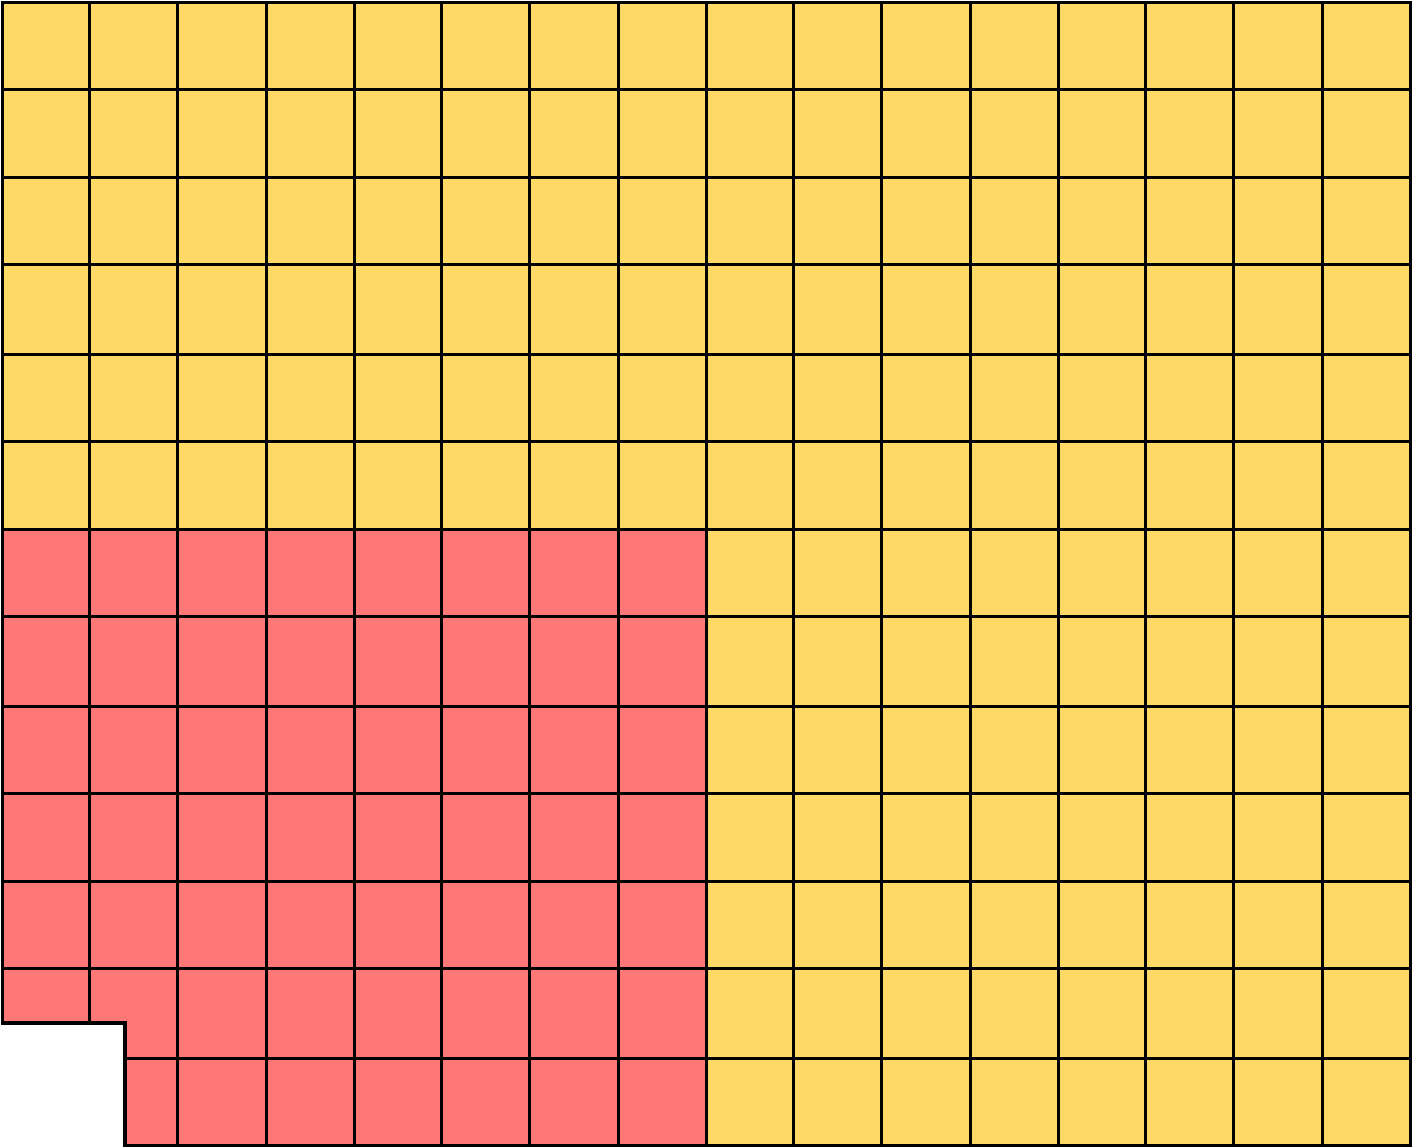
\includegraphics[width=0.48\textwidth]{HCAL}} \hfill
\caption{Representanciones gráficas de los calorímetros ECAL y HCAL.} \label{fig_calos}
\end{figure}

Tanto el ECAL como el HCAL, que pueden verse en la Figura \ref{fig_calos}, emplean el mismo principio de detección: captar centelleos de las partículas cargadas y transmitir estos fotones vía fibras de onda a tubos fotomultiplicadores. 
%
En el momento de identificar las partículas, el calorímetro provee al \texttt{L0} información combinada de ECAL, PS y SPD que permite la identifiación de partículas: el \texttt{CALO PID}.
%
Al igual que el RICH, se hacen tests para discriminar las partículas mediante medias de log--\emph{likelihood} calculadas con las deposiciones de energía en las distintas posiciones de los calorímetros.

%TRIGGER search triger and make it italic

\subsubsection{Sistema de muones} %%%%%%%%%%%%%%%%%%%%%%%%%%%%%%%%%%%%%%%%%%%%%%

Los muones son partículas muy penetrantes debido a su poca sección eficaz de interacción, y por ello pueden atravesar los calorímetros sin apenas perder más que una pequeña energía, pudiendo así detectarse al final de \lhcb, en las cámaras de muones. \color{new} El sistema de muones es empleado tanto en el \texttt{L0}--trigger, para seleccionar muones con un alto momento tranverso; y en la reconstrucción offline, para identificarlos. \color{norm}

El sistema de muones de \lhcb \cite{Alves:1129809} se compone de 5 estaciones, M1--M5: M1 se sitúa entre el RICH2 y el SPD, y usa tecnología de \emph{Gas Electron Multiplier} (GEM) puesto que en esta región hay una mayor tasa de partículas; las cámaras M2-M5 se encuentran después del HCAL y emplean \emph{Multiwire Proportional Chambers} (MWPC) \color{new} separados por $80$ cm de hierro. La aceptancia general del sistema de muones está entre $20 (16)$ mrad y $306 (258)$ mrad en el plano perpendicular (paralelo) al campo magnético. \color{norm}

\begin{figure}[H]
\centering
\includegraphics[width=0.6\textwidth]{MuonChamber.pdf}
\caption{Representación de un cuarto de la cámara de muones M1, en donde se pueden apreciar los \emph{pads} y las celdas detectoras. En cada región de las estaciones M2 y M3 (M4 y M5) el número de columnas detectoras de cada \emph{pad} es el doble (la mitad), manteniéndose constante el número de filas.}	\label{fig_muonchambers}
\end{figure}

La geometría de las diferentes estaciones varía el número de celdas detectoras en cada una, existiendo para cada estación zonas más y menos densas, tal y como puede apreciarse en la Figura \ref{fig_muonchambers}, acabando finalmente por computar un flujo similar en todas ellas.



%%%%%%%%%%%%%%%%%%%%%%%%%%%%%%%%%%%%%%%%%%%%%%%%%%%%%%%%%%%%%%%%%%%%%%%%%%%%%%%%

%TODO search fisica and change uppercase

%%%%%%%%%%%%%%%%%%%%%%%%%%%%%%%%%%%%%%%%%%%%%%%%%%%%%%%%%%%%%%%%%%%%%%%%%%%%%%%%
%%%%%%%%%%%%%%%%%%%%%%%%%%%%%%%%%%%%%%%%%%%%%%%%%%%%%%%%%%%%%%%%%%%%%%%%%%%%%%%%
\section{Sistema de trigger} %%%%%%%%%%%%%%%%%%%%%%%%%%%%%%%%%%%%%%%%%%%%%%%%%%%
%%%%%%%%%%%%%%%%%%%%%%%%%%%%%%%%%%%%%%%%%%%%%%%%%%%%%%%%%%%%%%%%%%%%%%%%%%%%%%%%
%%%%%%%%%%%%%%%%%%%%%%%%%%%%%%%%%%%%%%%%%%%%%%%%%%%%%%%%%%%%%%%%%%%%%%%%%%%%%%%%

\begin{wrapfigure}{r}{0.45\textwidth}
  \centering
  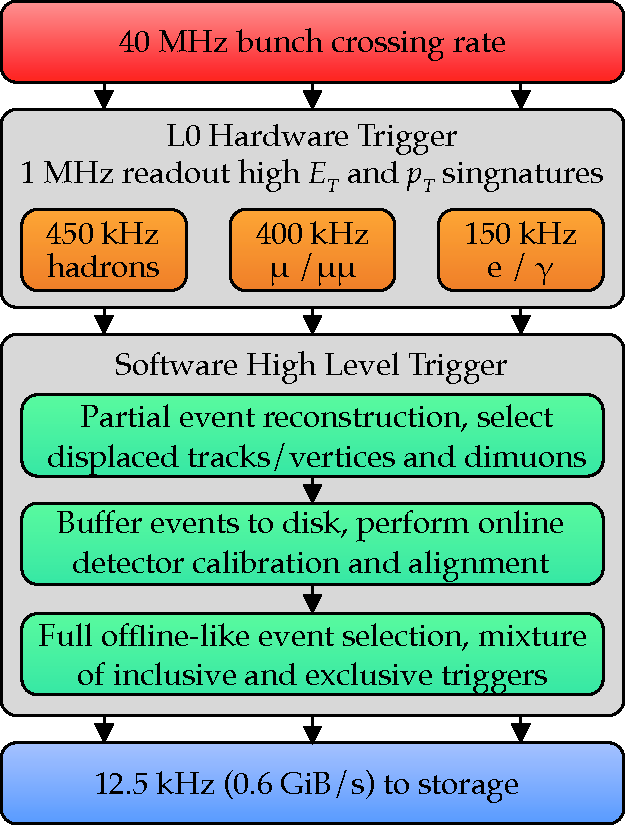
\includegraphics[width=0.4\textwidth]{Trigger.pdf}
  \caption{Esquema de actuación del \emph{trigger} de \lhcb en 2015.}	
\end{wrapfigure}

La frecuencia de colisión de \lhcb es de $40 \, \mathrm{M Hz}$, lo que se traduce en unos $10 \, \mathrm{M Hz}$ de eventos que entran en la aceptancia del detector. El número de \color{vero} eventos \color{norm} que puede ser grabado está limitado por la capacidad de cálculo \emph{offline}, de aproximadamente $2 \, \mathrm{k Hz}$, por lo que la cantidad de datos generada en  las colisiones de \lhc es demasiado alta para ser guardada directamente, y es por ello que se necesita de un eficaz sistema de \emph{trigger} que permita reducirla sin perder los eventos de mayor importancia para la Física. \color{new}
La estrategia principal del trigger se fundamenta en dos signaturas de las desintegraciones de los mesones B: la gran masa del B crea productos de desintegración con alto momento transverso $p_T$, y la larga vida media del B  genera productos con un parámetro de impacto grande respecto del vértice primario. \color{norm}
El sistema de trigger de \lhcb consta de dos niveles: \color{new} el Level--0 trigger (\texttt{L0}) de tipo hardware y el High Level Trigger (\texttt{HLT}) de tipo software \cite{Head_2014}. \color{norm}


%%%%%%%%%%%%%%%%%%%%%%%%%%%%%%%%%%%%%%%%%%%%%%%%%%%%%%%%%%%%%%%%%%%%%%%%%%%%%%%%
\subsection{Hardware trigger} %%%%%%%%%%%%%%%%%%%%%%%%%%%%%%%%%%%%%%%%%%%%%%%%%%
\label{sec_l0trigger}

La función del \texttt{L0} es reducir la tasa de datos a $1\,\mathrm{MHz}$, tasa a partir de la cual el detector se puede leer completamente. La decisión de si se debe o no aceptar el evento la toma la \textit{Decision Unit} (DU), basada en la información que síncronamente se está viendo en el detector a $40\,\mathrm{MHz}$. Para ello se usa la información siguiente:
\begin{itemize}
  \item \texttt{L0Calo}: Se toma la energía transversa de los \textit{clusters} que se producen en el calorímetro por los electrones, fotones, piones neutros y hadrones cargados. %esta se calcula en célus $2\times2$ .....
  \item \texttt{L0Muon}:  Se toma el momento transverso, $p_T$, de los muones o dimuones, llevándose a cabo una reconstrucción rápida de los candidatos con una resolución del $20 \, \%$. La DU solo hará uso de los dos candidatos con el $p_T$ más alto.
  \item Multiplicidades en el SPD: El número total de celdas del detector SPD que tienen un \textit{hit} se usa para obtener la multiplicidad de carga de la traza y rechazar así los eventos con un número muy alto de multiplicidades, que saturaría al \texttt{HLT} en la siguiente etapa.
\end{itemize}
%
Toda esta información se transmite a la \texttt{L0}DU, y se traduce con la calibración y triggers aleatorios en una decisión con una latencia máxima de $1 \, \mathrm{\upmu s}$. La decisión se envía a la electrónica \emph{front--end}, y si es positiva la electrónica de los detectores toma los datos y los envía a la EFF.



%%%%%%%%%%%%%%%%%%%%%%%%%%%%%%%%%%%%%%%%%%%%%%%%%%%%%%%%%%%%%%%%%%%%%%%%%%%%%%%%
\subsection{Software Trigger} %%%%%%%%%%%%%%%%%%%%%%%%%%%%%%%%%%%%%%%%%%%%%%%%%%
\label{sec_hltrigger}

Los datos aceptados por el \texttt{L0} se transmiten a la EFF, donde se ejecuta el \texttt{HLT}. El \texttt{HLT} es una aplicación \texttt{C++} que corre en cada CPU de la EFF y reduce la tasa de datos de 1 MHz hasta 12.5 kHz (en 2015). El \texttt{HLT} realiza una reconstrucción total de las trazas usando información \color{vero} de \color{norm} todo el detector, buscando discriminar la señal del ruido. \color{vero} Opera en dos \color{norm} partes:

\begin{itemize}
  \item \texttt{HLT1}: Usa información del VELO y las estaciones de trazado para reconstruir la traza 3D de la partículas y obtener el PV. Además se realiza una reconstrucción rápida de las trazas en las cámaras de muones, y se hace uso del parámetro de impacto, el momento total y transverso así como las deposiciones de energía en los calorímetros para reducir todavía más la tasa de datos.
  \item \texttt{HLT2}: A este nivel se puede reconstruir  totalmente el evento; se alcanzan los $12.5$ kHz que se graban para su posterior análisis, con una tasa de almacenamiento de $0.6 \, \mathrm{GiB s^{-1}}$.
\end{itemize}

\color{dieg}
El \texttt{HLT} funciona con las denominadas \emph{trigger lines}: cortes y criterios de selección similares a los aplicados durante los análisis. La implementación de las mismas puede ser bastante general o ceñirse a características más específicas. Por ejemplo, una línea de trigger puede exigir la presencia de dos muones, formando un vértice con una masa invariante en la ventana de masa de $\Jpsi$. \color{norm}

 \todo[inline]{meter líneas de jpsikk.}
 

Concretamente para el canal aquí estudiado, $\Bs \to \Jpsi \kaon \antikaon$, se aceptan todos los eventos que superen los criterios del \texttt{L0}. En  lo que al \texttt{HLT} concierne, existen dos categorías \cite{paperPhis}:
\begin{itemize}
  \item \texttt{Unbiased}: Se exige la correcta identificación de dos muones de carga opuesta con masa invariante mayor de $2700 \,\mathrm{MeV/}c^2$. La aceptancia en esta categoría es prácticamente constante, como puede verse en \S \ref{REF}.
  \item \texttt{Biased}: Se aceptan eventos si existe al menos un muón con momento transverso mayor de $1 \mathrm{GeV/}c$, y con un parámetro de impacto significativo respecto de los demás vértices primarios de ese evento; o bien, si se pasa la selección de un algoritmo multivariado que  identifica trazas de dos partículas, con un vértice secundario de suma de momento transverso alto y significativamente separado del vértice primario.
\end{itemize}

%%%%%%%%%%%%%%%%%%%%%%%%%%%%%%%%%%%%%%%%%%%%%%%%%%%%%%%%%%%%%%%%%%%%%%%%%%%%%%%%



%%%%%%%%%%%%%%%%%%%%%%%%%%%%%%%%%%%%%%%%%%%%%%%%%%%%%%%%%%%%%%%%%%%%%%%%%%%%%%%%
%%%%%%%%%%%%%%%%%%%%%%%%%%%%%%%%%%%%%%%%%%%%%%%%%%%%%%%%%%%%%%%%%%%%%%%%%%%%%%%%
%%%%%%%%%%%%%%%%%%%%%%%%%%%%%%%%%%%%%%%%%%%%%%%%%%%%%%%%%%%%%%%%%%%%%%%%%%%%%%%%
  \cleardoublepage%%%%%%%%%%%%%%%%%%%%%%%%%%%%%%%%%%%%%%%%%%%%%%%%%%%%%%%%%%%%%%%%%%%%%%%%%%%%%%%%
%%%%%%%%%%%%%%%%%%%%%%%%%%%%%%%%%%%%%%%%%%%%%%%%%%%%%%%%%%%%%%%%%%%%%%%%%%%%%%%%
%%%%%%%%%%%%%%%%%%%%%%%%%%%%%%%%%%%%%%%%%%%%%%%%%%%%%%%%%%%%%%%%%%%%%%%%%%%%%%%%
\chapter{Herramientas y técnicas de análisis}
\label{cha:tools}
%%%%%%%%%%%%%%%%%%%%%%%%%%%%%%%%%%%%%%%%%%%%%%%%%%%%%%%%%%%%%%%%%%%%%%%%%%%%%%%%
%%%%%%%%%%%%%%%%%%%%%%%%%%%%%%%%%%%%%%%%%%%%%%%%%%%%%%%%%%%%%%%%%%%%%%%%%%%%%%%%
%%%%%%%%%%%%%%%%%%%%%%%%%%%%%%%%%%%%%%%%%%%%%%%%%%%%%%%%%%%%%%%%%%%%%%%%%%%%%%%%

\section{Herramientas de simulación}

La importancia de tener una muestra de datos simulados tiene diversos motivos. Primeramente, permite entrenar a las herramientas que después se usarán sobre datos reales, pero teniendo conocimiento completo del proceso estudiado. Por otra parte, el proceso de detección es preciso, pero no perfecto, lo que produce que aparezcan desviaciones en las distribuciones físicas. Para tener en cuenta estos efectos, y corregirlos, se emplean simulaciones completas de \lhcb del canal en concreto a estudiar: el \emph{full} Monte Carlo.

\begin{figure}[H]
\centering
\includegraphics[width=0.95\textwidth]{GaussApplication.pdf}
\caption{Estructura de la aplicación \textsc{Gauss}.}	 \label{fig_gaussapp}
\end{figure}

En \lhcb la aplicación \color{dieg} encargada \color{norm} de llevar a cabo la generación y transporte de partículas a través del detector es \textsc{Gauss} \cite{Clemencic_2011}. Esta herramienta funciona en dos bloques separadamente que pueden ser operados en conjunto (\emph{vid.} Figura \ref{fig_gaussapp}):
\begin{itemize}
	\item Generación de eventos: Las colisiones protón--protón son generadas usando \pythia \cite{sjostrand2015introduction}, con una configuración específica para \lhcb. Las desintegraciones de partículas son descritas con \eviltgen \cite{Lange:2001uf} y la radiación de las partículas en el estado final son generadas por \photos \cite{golonka2006photos}.
	\item Simulación del detector: La interacción entre las partículas generadas con el detector, y la respuesta de este mismo, la describe \geant \cite{Agostinelli:2002hh}.
\end{itemize}


El proceso de generación y reconstrucción de trazas es computacionalmente costoso y se realiza en el GRID de \lhcb. 
El GRID de \lhcb se compone de una red internacional de computadores conectados cuyo objetivo principal es el análisis de datos del experimento. Al sistema de computación distribuida puede accederse desde \textsc{Dirac} o mediante \textsc{Ganga}, dos herramientas que hacen de interfaz con el usuario y el sistema de colas.

%Este es un hecho de capital importancia puesto que, de este modo, estos recursos son comunes a todos los físicos que analizan datos.


%De hecho, la cantidad limitada de MC viene siendo la principal contribución a la incertidumbre sistemática de $\phi_s$.







\section{Estimación por máxima verosimilitud}


Para extraer parámetros de conjuntos de datos, como las que se muestran en la Figura \ref{fig_evtgensamples1}, se emplean algoritmos de ajuste (\emph{fit}). Existen diversos métodos para poder minimizar un funcional respecto de una muestra y extraer los parámetros, entre ellos aquí se emplea el método de máxima verosimilitud.

El método de máxima verosimilitud \cite{cowan}, MLE, es una técnica para estimar los valores de parámetros \emph{verdaderos}, $\theta_k^0$, de una muestra finita de datos, $x_i$, dada. Si la medida se repite $N$ veces, entonces $x_i$ tendrá $N$ valores para la dimensión $i$ (pudiendo tener una variable más dimensiones).



Asumiendo la hipótesis de la función de densidad de probabilidad, \emph{p.d.f.}, para la muestra $x$, y siendo todas las medidas independientes, se verifica que
\begin{equation}
\text{probabilidad de } \quad x_i \in [x_i, x_i+dx_i] \quad \forall i \quad  = \quad \prod_{i=1}^N f(x_i,\theta_k) dx_i	
\end{equation}




Si la hipótesis es correcta y los parámetros son $\theta_k \approx \theta_k^0$, se espera una alta probabilidad para los datos medidos. Mismamente, si los parámetros se alejan del valor verdadero $\theta_k^0$, entonces se obtendrá una baja probabilidad.
Como  $dx_i$ no depende de los parámetros, se define la función de verosimilitud como
\begin{equation}
	L(\theta_k) = \prod_{i=1}^N f(x_i,\theta_k) \label{eq_likelihood_def}
\end{equation}  
que no es más que la \color{dieg} $p.d.f.$ conjunta de $x_i$ como función de los parámetros a estimar. \color{norm} Los datos actúan como constantes, puesto que el experimento ha finalizado.


En virtud de la Ecuación (\ref{eq_likelihood_def}), 
uno define el método de máxima verosimilitud (MLE), escogiendo maximizar la función de verosimilitud, \emph{likelihood}. Se trata por tanto de buscar
\begin{equation}
	\frac{\partial L(\theta_k)}{\partial \theta_k} = 0, \qquad k=\{1,\dots,N\}.
\end{equation}

\begin{figure}[H]
\centering
\includegraphics[width=0.9\textwidth]{MLfit.pdf}
\caption{Ejemplo conceptual del ajuste por máxima verosimilitud. Se ajustan unos ciertos datos respecto de una \textit{p.d.f.} gaussiana, cuyo valor del parámetro media coincide con la media de la muestra, y ello se corresponde con el máximo de la veroslimilitud.} \label{fig_maxloglikeexp}
\end{figure}	
%TODO make new picture here






\section{Minimizar}

Para realizar los ajustes por máxima verosimilitud, se requiere de un algoritmo capaz de encontrar extremos relativos de funciones que sea lo suficientemente sofisticado para manejar grandes cantidades de datos y funciones de varios parámetros. 


\subsection{Paralelización}



\color{dieg}
Gran parte del coste computacional  del análisis recae en el cálculo de la \emph{likelihood}, que luego se optimiza.  
%
La minimización puede ser un proceso lento, sobre todo con grandes cantidades de datos y parámetros, y más cuando se procede vía un ajuste multidimensional. Es aquí donde la paralelización se vuelve de gran ayuda. Típicamente una CPU tiene del orden de 10 \textit{cores}, en los que se pueden paralelizar procesos, mientras que una GPU tiene del orden de 100 veces más \textit{cores}. 

La paralelización se realiza por eventos, calculándose la \emph{likelihood} en la GPU para cada conjunto de parámetros y llevándose a cabo la minimización en la CPU con \minuit \cite{James:1975dr},  un minimizador de tipo gradiente que busca mínimos de funciones y es reconocido como uno de los mejores algoritmos de su tipo. 
\color{norm}

Para este trabajo se emplearon GPUs de la marca \textsc{nVidia}, y que son relativamente fáciles de usar, puesto que la propia compañía ofrece \textsc{cuda}, un \textit{framework} que permite usar las tarjetas programando en \texttt{cuda}--\texttt{C}, muy similar a \texttt{C}.
%
Al final se emplea \texttt{Python} como una interfaz y gestor de datos en la CPU, empleando para ello la librería \texttt{PyCuda}; existiendo además un paquete de software llamado \texttt{Ipanema} \cite{santos2017ipanema}, con funcionalidades adecuadas a esta línea de trabajo. Desde el punto de vista técnico, se necesita de la CPU para coordinar todos los procesos y de un código que la GPU entienda, en donde se indiquen las posiciones y operaciones que deben hacerse sobre \emph{arrays} de datos, así como una forma óptima de salida del programa. Puede verse un esquema de como operan las diferentes parte en la Figura \ref{fig:CPUioGPU}.





\begin{figure}[H]
  \centering
  \includegraphics[width=0.9\textwidth]{CPUioGPU.pdf}
  \caption{Esquema del flujo de trabajo e interacciones entre el usuario, la CPU y la GPU con \texttt{Ipanema}. Aquí FCN se refiere al valor de la función a cada llamada de la CPU, y es el número a minimizar con Miniuit.} \label{fig:CPUioGPU}
\end{figure}


\subsection{\textsc{Minuit}}

\textsc{Minuit} es un algoritmo escrito por F. James en la década de los 70 en el CERN. Fue concebido como una herramienta para encontrar el mínimo de funciones multiparamétricas y analizar la forma de la función alrededor del mínimo. Su principal aplicación es el análisis estadístico de datos, principalmente para obtener el mejor conjunto de parámetros que minimice un $\chi^2$ o maximice la verosimilitud. Además de estimar los parámetros, computa sus incertidumbres estadísticas y la correlación entre ellos. Es especialmente útil para problemas difíciles, incluyendo aquellos que requieran de ser guiados para hallar la solución correcta 
\cite{James:1975dr}.

Brevemente, las funciones que \texttt{Minuit} aporta son:
\begin{itemize}
  \item \texttt{Migrad}: Encuentra, empleando la fórmula Davidon–Fletcher–Powell (DFP), el conjunto de parámetros que minimiza un funcional dado sobre unos datos.
  \item \texttt{Hesse}: Estima con mayor precisión la hessiana, extrayéndose de esta parte las incertidumbres parabólicas de los parámetros obtenidos con \texttt{Migrad}.   
  \item \texttt{Minos}: En problemas complicados es plausible que la función a minimizar no sea simétrica respecto de un parámetro alrededor del mínimo (como presupone \texttt{Hesse}), por ello esta función, computacionalmente más costosa, estima la incertidumbre asimétrica de los parámetros.
\end{itemize}



\subsection{Fórmula de Davidon--Fletcher--Powell}

El algoritmo DFP fue desarrollado por Davidon (1959), Fletcher y Powell (1963), y es también conocido como el \emph{variable metric algorithm} \cite{fletcher1963rapidly}. Se trata de una generalización de los métodos \textit{quasi}--Newton, que asegura que se preserve que la hessiana sea definida positiva.

Considérense la función $f(x)$ y su gradiente $\nabla f$, y la matriz hessiana $H$, la serie de Taylor de la función $f$ es \cite{fletcher2000practical}
\begin{equation}
  f(x_k+s_k) = f(x_k) + \nabla f(x_k)^T s_k + \frac{1}{2} s_k^{\top} {H} s_k + \dots,
\end{equation}
y para su gradiente (ecuación secante), que es usado para calcular la hessiana es
\[\nabla f(x_k+s_k) = \nabla f(x_k) + H s_k + \dots\,.\]
  

La fórmula DFP encuentra la solución a la ecuación secante que es más próxima al valor estimado y que además verifica la condición de curvatura, cumpliendo que la hessiana sea simétrica y definida positiva
\begin{equation}
  H_{k+1}=
(I - \gamma_k y_k s_k^{\top}) H_k (I - \gamma_k s_k y_k^{\top}) + \gamma_k y_k y_k^{\top},
\end{equation}
donde $y_k = \nabla f(x_k+s_k) - \nabla f(x_k),$ con 
$\gamma_k = \frac{1}{y_k^{\top} s_k}$.

A cada iteración la aproximación a la inversa de la hessiana $G_k = G_k^{-1}$ es
\begin{equation}
  G_{k+1} = G_k - \frac{G_k y_k y_k^{\top} G_k}{y_k^{\top} G_k y_k} + \frac{s_k s_k^{\top}}{y_k^{\top} s_k}.
\end{equation}
donde se asume que $H$ es definida positiva, cumpliendo los vectores  $s_k^T$ e $y$ la condición de curvatura
\begin{equation}
  s_k^{\top} y_k = s_k^{\top} H s_k > 0.
\end{equation}

La fórmula DFP es muy efectiva, y de hecho fue el primer método \textit{quasi}--Newton en generalizar el método de la secante para un problema multidimensional. Sin embargo, para grandes problemas no cuadráticos, el algoritmo puede estancarse; un fenómeno atribuido a que $H$ se vuelve una matriz casi singular. Notar que a pesar de ello es mejor la fórmula Broyden--Fletcher--Goldfarb--Shanno, que es dual (bajo el intercambio $y$ y $s$).



\begin{figure}[H]
  \centering
  \includegraphics[width=0.7\textwidth]{rosen.pdf}
  \caption{Minimización de la función de Rosenbrock mediante el método DFP. Se situó la semilla en $(-0.5,3)$, y se halló el mínimo de $f(x, y) = (a-x)^2 + b(y-x^2)^2$ en $(1,1)$ para los parámetros $a=1$ y $b=100$.}
\end{figure}



\section{Splines}

Los splines son funciones polinómicas definidas a trozos, que resultan particularmente útiles para interpolar datos con formas complicadas y que pueden tener ruido. Existen diferentes formas de construir splines, aquí se centrará el texto en los \textit{basis} splines con polinomios de tercer orden.


\subsection{B-splines}

Dado un conjunto de nodos, $k = \{u_0,\dots,u_n\}$, con $n+1$ elementos que definen $n$ intervalos, para un spline cúbico hay $n+3$ parámetros, $b$, que lo definen \cite{Weisstein}. La función interpolante  se construye como la suma lineal de b--splines \cite{paperPhis}
\begin{equation}
s(u) = \sum_{i=0}^{n+2}  b_i s_i(u).
\end{equation}
%
Para un valor $u$ en un determinado intervalo, $u \in (u_i,u_{i+1}]$, contribuyen cuatro b--splines, concretamente, $s_i(u)$ con $i \in \{i,i+1,i+2,i+3\}$. Es preciso extender los nodos en los extremos para calcular dichas contribuciones,
\[u_{i} = u_0 \,\,\, \forall i<0 \qquad \text{y} \qquad u_{i} = u_{n} \,\,\, \forall i>n.\]

Definiendo, la variable $\delta$ \cite{paperPhis},
\begin{equation}
  \delta_i(u) = u - u_i \qquad \qquad \delta_i^j = u_j -u_i
\end{equation}
se pueden escribir las cuatro contribuciones no nulas como,
\begin{equation}
  s_i(u) = b_i A_i(u) + b_{i+1} B_i + b_{i+2} C_i + b_{i+3} D_i 
\end{equation}
donde
\begin{equation}
\begin{split}
  A_i(u)&= -\frac{ \delta_{i+1}(u) ^3}
                 { \delta_{i-2}^{i+1} \delta_{i-1}^{i+1} \delta_{i  }^{i+1}}\\
  B_i(u)&=  \frac{ \delta_{i-2}(u) \delta_{i+1}(u)^2 }
                 { \delta_{i-2}^{i+1} \delta_{i-1}^{i+1} \delta_{i  }^{i+1}} 
           +\frac{ \delta_{i-1}(u) \delta_{i+1}(u) \delta_{i+2}(u) }
                 { \delta_{i-1}^{i+2} \delta_{i-1}^{i+1} \delta_{i  }^{i+1}} 
           +\frac{ \delta_{i}(u) \delta_{i+2}(u)^2 }
                 { \delta_{i  }^{i+2} \delta_{i-1}^{i+2} \delta_{i  }^{i+1}} \\
  C_i(u)&=  \frac{ \delta_{i-1}(u)^2 \delta_{i+1}(u) }
                 { \delta_{i-1}^{i+2} \delta_{i-1}^{i+1} \delta_{i  }^{i+1}} 
           +\frac{ \delta_{i-1}(u) \delta_{i}(u) \delta_{i+2}(u) }
                 { \delta_{i  }^{i+2} \delta_{i-1}^{i+2} \delta_{i  }^{i+1}} 
           +\frac{ \delta_{i}(u)^2 \delta_{i+3}(u) }
                 { \delta_{i  }^{i+3} \delta_{i  }^{i+2} \delta_{i  }^{i+1}} \\
  D_i(u)&=  \frac{ \delta_{i}(u) ^3}
                 { \delta_{i  }^{i+3} \delta_{i  }^{i+2} \delta_{i  }^{i+1}}.
\end{split}
\end{equation}
De este modo, fijando un conjunto de nodos, se han de encontrar los parámetros $b$. Por simplicidad a la hora de ser implementado, es útil considerar
\begin{equation}
   b_i A_i(u) + b_{i+1} B_i + b_{i+2} C_i + b_{i+3} D_i = \beta_0 + \beta_1 u + \beta_2 u^2 + \beta_3 u^3
\end{equation}
donde los coeficientes $\beta_i$ son propios de cada bin, a diferencia de los $b_i$, que son comunes a todo el spline. 


%\begin{equation}
%  P = \delta_{i-2}^{i+1} \delta_{i-1}^{i+1} \delta_{i  }^{i+1}
%  Q = \delta_{i-1}^{i+2} \delta_{i-1}^{i+1} \delta_{i  }^{i+1}
%  R = \delta_{i  }^{i+2} \delta_{i-1}^{i+2} \delta_{i  }^{i+1}
%  S = \delta_{i  }^{i+3} \delta_{i  }^{i+2} \delta_{i  }^{i+1}
%\end{equation}

%\subsection{\emph{Smoothing} splines}
%
%Los \textit{smoothing} splines son funciones de estimación que se obtienen a partir de una cierta muestra de observaciones $y_i$  para un determinado modelo $f(x_i)$ \cite{reinsch1967smoothing}.
%
%Considerando un conjunto de nodos (\emph{knots}) $\{k_i\}_{i=0}^{n-1}$ y que existe la relación $y_i = f(k_i) + \epsilon_i$ , donde $\epsilon_i$  son variables aleatorias de media cero y de varianza constante. El \textit{smoothing} spline $\hat{f}$ es la estimación de la función $f$, penalizando el salto de la segunda derivada
%\begin{equation}
%\chi^2(\lambda) = \sum_{i=0}^{n-1} \left(\frac{y_i - \hat f(x_i)}{\sigma_i}\right)^2 + \lambda \int \hat f''(x)^2 \,dx,
%\end{equation}
%donde $\lambda$ es el parámetro de suavizado que controla la relevancia de la integral de las segundas derivadas.
%
%A medida que $\lambda \rightarrow 0$, el \textit{smoothing} spline converge al spline interpolante. Por otra parte, según $\lambda \rightarrow \infty$, la penalización sobre las rugosidades se vuelve cada vez más importante y el \textit{smoothing} spline converge a un ajuste  lineal por mínimos cuadrados.
%
%Con los splines se puede suavizar el ruido en datos $(x_i,y_i)$, resultando en splines menos rugosos. Resulta particularmente interesante el caso de los splines cúbicos, que además de su buen funcionamiento, simplifican el proceso \cite{paperPhis}. 
%
%
%
%\subsubsection*{B--splines cúbicos suavizados}
%
%Si se consideran b-splines cúbicos, entonces el término de penalización se simplifica. Como los coeficientes de los splines están totalmente determinados por los $\hat f (k_i)$, el problema se puede separar en dos partes:
%\begin{enumerate}%[(i)]
%  \item Obtener un conjunto de puntos $(k_i,\mu_i = \hat f (k_i))$, construyendo un spline interpolante entre $(k_i,y_i)$.
%  \item A partir de $\mu_i$, construir un B--spline $ \hat{f}(x)$, para todo $x$.
%\end{enumerate}
%
%Como la derivada segunda de un B--spline cúbico es una función lineal, entonces se sigue que el término de penalización se puede escribir como una forma cuadrática,
%\begin{equation}
%\int \hat f''(x)^2 dx = \mu^{\top} \textbf{M} \,\mu.
%\end{equation}
%donde la matriz $\textbf{M}$ (de dimensión $n\times n $), puede expresarse como $\textbf{M} = \textbf{V}^{\top} \textbf{W}^{-1} \textbf{V}$. 
%%
%%
%La matriz $\textbf{V}$, de dimensión $(n-2)\times n$, y se construye con elementos de segundas diferencias,
%\begin{equation*}
%V = \begin{pmatrix}
%\frac{1}{h_1} & -\left(\frac{1}{h_1}+\frac{1}{h_{2}}\right) & \frac{1}{h_{2}} & 0 & \cdots & 0 \\
%0 & \frac{1}{h_i} & -\left(\frac{1}{h_i}+\frac{1}{h_{i+1}}\right) & \frac{1}{h_{i+1}} & \cdots & 0 \\
%\vdots & \vdots & \ddots & \ddots & \ddots & \vdots \\
%0 & 0 & \cdots & \frac{1}{h_{n-2}} & -\left(\frac{1}{h_{n-2}}+\frac{1}{h_{n-1}}\right) & \frac{1}{h_{n-1}} 
%\end{pmatrix}
%\end{equation*}
%%
%%
%La matriz $\textbf{W}$, simétrica, tridiagonal y de dimensión $(n-2)\times(n-2)$, se construye con las distancias entre nodos sucesivos
%\begin{equation*}
%W = \begin{pmatrix}
%\frac{h_0+h_{1}}{3}  & \frac{h_0}{6} & 0 & \cdots & 0 \\
%\frac{h_i}{6} & \frac{h_i+h_{i+1}}{3}  & \frac{h_i}{6} & \cdots & 0 \\
%\vdots & \ddots & \ddots & \ddots & \vdots \\
%0 & 0 & \cdots & \frac{h_{n-3}}{6} & \frac{h_{n-3}+h_{n-2}}{3} 
%\end{pmatrix}
%\end{equation*}
%
%
%Entonces se aplica el paso (\textsc{i}) y la suma de cuadrados se puede escribir como
%\[\chi^2(\lambda) = \sum_{i=0}^{n-1} \left(\frac{y_i - \hat f(x_i)}{\sigma_i}\right)^2 + \lambda \vec{\mu}^{\top} \textbf{M} \,\vec{\mu}. \]
%Esto implica que $\chi^2 (\lambda)$ es una función de segundo orden en $\mu$ y por lo tanto su minimización resulta de optimizar el sistema 
%\begin{equation}
%  \left(\Sigma^{-1} - \lambda \textbf{M} \, \right) \mu = \Sigma^{-1} Y, \qquad \Sigma^{-1} = \text{diag}(1/\sigma_i).
%\end{equation}
%Resolviendo dicho sistema, se puede obtener un conjunto \textit{smooth} $\mu_i$, que luego se puede usar para construir un B--spline interpolante ---paso (\textsc{ii}).
%
%









  \cleardoublepage%%%%%%%%%%%%%%%%%%%%%%%%%%%%%%%%%%%%%%%%%%%%%%%%%%%%%%%%%%%%%%%%%%%%%%%%%%%%%%%%
%%%%%%%%%%%%%%%%%%%%%%%%%%%%%%%%%%%%%%%%%%%%%%%%%%%%%%%%%%%%%%%%%%%%%%%%%%%%%%%%
%%%%%%%%%%%%%%%%%%%%%%%%%%%%%%%%%%%%%%%%%%%%%%%%%%%%%%%%%%%%%%%%%%%%%%%%%%%%%%%%
\chapter[Actualización del modelo $\Bs \rightarrow \text{J}/\uppsi \antikaon\kaon$][Actualización del modelo $\bm{\Bs \rightarrow \text{J/}}\text{ψ}  \bm{\antikaon\kaon}$]{Actualización del modelo $\bm{\Bs \rightarrow \text{J/}}\text{ψ}  \bm{\antikaon\kaon}$}
\label{cha:evtmodel}


%%%%%%%%%%%%%%%%%%%%%%%%%%%%%%%%%%%%%%%%%%%%%%%%%%%%%%%%%%%%%%%%%%%%%%%%%%%%%%%%
%%%%%%%%%%%%%%%%%%%%%%%%%%%%%%%%%%%%%%%%%%%%%%%%%%%%%%%%%%%%%%%%%%%%%%%%%%%%%%%%
%%%%%%%%%%%%%%%%%%%%%%%%%%%%%%%%%%%%%%%%%%%%%%%%%%%%%%%%%%%%%%%%%%%%%%%%%%%%%%%%

\todo[inline]{poner inputs para cada MC y así comparar con el fit}

En el marco concreto  de este trabajo se creó un nuevo modelo de \texttt{EvtGen}, para simular el canal $\Bs \rightarrow \Jpsi \antikaon\kaon$, con capacidad para crear y desintegrar las resonacias $\fzero$, $\fai$ y $\ftwop$, y \color{vero} generar también la interferencia entre ellas. \color{norm} 

El modelo debe incorporar las distribuciones angulares de la \S \ref{sec_angdist}, la evolución temporal de la \S \ref{sec_tempdist}, y las distribuciones de masa para las partículas de ondas S (no resonante), S ($\fzero$), P($\fai$) y D($\ftwop$), que aparecen en \S \ref{sec_diffrate}.  Todas estas funciones se escriben en \texttt{C++}, y se adecúan para ser integradas en el software de \lhcb, \textsc{Gauss}. 

\section{Parámetros de desintegración}

Para poder interaccionar con el modelo, se compone también un \texttt{DecFile}, en el cual se escribe la lista de parámetros que constituyen la entrada al simulador.

\begin{table}[H]
\centering
\resizebox{\textwidth}{!}{\begin{tabular}{r|c|c|c|c|c|l}
nombre del canal & $f$ &$f_f$ & $\delta$ & $\phi_s$ &$\lambda$  \\ \hline
\texttt{1.0    mu+ mu-  K+    K-     BS\_MUMUKK} 
%
&   \texttt{0.00},& & \texttt{0.00,}& \texttt{-0.8,}& \texttt{1.0,}	\\
&  \texttt{0.50,} &                 & \texttt{3.32,}& \texttt{-0.8,}& \texttt{1.0,} \\
  &  \texttt{0.50,} & \texttt{0.509,} & \texttt{0.00,}   &\texttt{-0.8,} &  \texttt{1.0,}\\ 
  &                 & \texttt{0.260,} & \texttt{3.08,} & \texttt{-0.8,} & \texttt{1.0,} \\
 &                 &                 & \texttt{3.26,} & \texttt{-0.8,} & \texttt{1.0,}\\
 &                 & \texttt{0.468,} & \texttt{0.00,}   & \texttt{-0.8,} & \texttt{1.0,}\\
 &                 & \texttt{0.194,} & \texttt{3.08,} & \texttt{-0.8,} & \texttt{1.0,}\\
 &                 &                 & \texttt{3.26,} & \texttt{-0.8,}& \texttt{1.0,} &
 \texttt{0.6603, 0.08, 17.7,        
0.9499, 0.99, 1.05;}\\ \hline
&&&&&& $\Gamma$ \hspace*{6.5mm} $\Delta \Gamma$  \hspace*{4mm} $\Delta m$  \hspace*{2mm} $$   \hspace*{3mm}$m_{f_0} $\,\,\,$m_{\text{KK}}^{\text{mín}}$   $m_{\text{KK}}^{\text{máx}}.$  %\hspace*{0.2mm}
\end{tabular}}
\caption{Parámetros y valores de los mismos declarados en el \texttt{DecFile}. Se puede hallar una descripción detallada en el texto.} \label{tab:decfiles}
\end{table}

El primer bloque que se indica en ta Tabla \ref{tab:decfiles} indica el nombre del canal y las partículas involucradas. El siguiente bloque controla los parámetros de la distribución angular, las fracciones, fases y parámetros de violación CP. La primera columna, $f$, son las fracciones de cada una de las amplitudes onda S, P y D; por normalización se construye la fracción de onda D como $f_{D} = 1-f_{S}-f_{P}$. La segunda columna, $f_f$ indica la fracción de cada polarización que existe en una amplitud dada, por ejemplo la fracción de $f_{P\parallel} = 1-f_{P0}-f_{P\perp} = 1-0.509-0.260$. Seguidamente en la tercera y cuarta columna se definen $\delta$ y $\phis$, una para cada polarización y en radianes. La quinta columna de este bloque indica el parámetro de violación CP, $|\lambda|$, definiéndose uno para cada polarización. El último bloque controla la parte de la mezcla y desintegración, $\Gamma\,(\mathrm{ps^{-1}})$ , $\Delta \Gamma \,(\mathrm{ps^{-1}})$ y $\Delta m \,(MeV/)c^2$); el valor del polo de $\fzero$, $m_{f_0}$ (GeV/$c^2$); así como la ventana de masa en la que se generan los datos, $[m_{\text{KK}}^{\text{mín}},m_{\text{KK}}^{\text{máx}}]$ (GeV/$c^2$).


\section{Simulaciones}

En la \S \ref{sec_diffrate}, se calcula la tasa de decaimiento diferencial respecto de los ángulos de helicidad y del tiempo, y pueden verse muestras generadas con \textsc{Gauss} en la Figura \ref{fig_evtgensamples1}. \textsc{Gauss} genera los cuadrimomentos de las partículas, llamados vectores Lorentz, 
\[p_{\mu} = (p_0, \vec{p}) = (Ec^{-1},\vec{p})\]
de modo que es sencillo calcular la masa, empleando la \emph{pseudo}norma del vector de Lorentz
\[p^{\mu}p_{\mu} = \frac{E^2}{c^2} - |\vec{p}|^2 = m^2c^2. \]
Entonces, para el espectro de masa $\antikaon\kaon$, se suman las componentes los momentos de los dos kaones calculándose la masa con el cuadrivector suma; análogamente para el $\Jpsi\kaon$, se suman las del $\kaon$ y de los muones.

En la Figura \ref{fig_evtgensamples2} puede observarse el espacio fásico en el Dalitz \textit{plot} que representa $M_{\Jpsi\kaon}$ \emph{vs.} $M_{\antikaon\kaon}$, y donde se aprecian las diferentes contribuciones que fueron implementadas.




\begin{figure}[H]
\begin{flushright}
\begin{multicols}{2}
\includegraphics[width=\columnwidth]{plots/time} \\
\includegraphics[width=\columnwidth]{plots/hel_costhetaK} \\
\includegraphics[width=\columnwidth]{plots/mkk} \\
\includegraphics[width=\columnwidth]{plots/hel_phi} \\
\includegraphics[width=\columnwidth]{plots/hel_costhetamu} \\
\includegraphics[width=\columnwidth]{plots/mjpsik}
\end{multicols}
\end{flushright}
\caption{Histogramas de algunas de las variables simuladas. Las muestras de $5\times10^5$ eventos  son \emph{sin} onda D (azul), con $7\,\%$ S onda y $93\,\%$ P \emph{wave} en la ventana de masa $m_{\text{KK}} = [0.98,1.20]\,\mathrm{GeV}/c^2$; y \emph{con} onda D (verde), con $15\,\%$ S \emph{wave} y $70\,\%$ P \emph{wave} y $15\,\%$ D \emph{wave} en el rango de masa $m_{\text{KK}} = [1.0,2.2]\,\mathrm{GeV}/c^2$.}   \label{fig_evtgensamples1}
\end{figure}





\begin{figure}[H]
\centering
\includegraphics[width=0.9\textwidth]{plots/dalitz1}
\includegraphics[width=0.9\textwidth]{plots/dalitz2}
\caption{Dalitz \textit{plot} para dos muestra de $5\times 10^5$ eventos, arriba con $15\,\%$ S \emph{wave}, $70\,\%$ P \emph{wave} y $15\,\%$ D \emph{wave} y abajo $11\,\%$ S \emph{wave}, $89\,\%$ P \emph{wave}. Se aprecian claramente las resonancias $\fai$ y $\ftwop$. Alrededor del $\fai$, puede verse también $\fzero$ de una forma más difusa.}   \label{fig_evtgensamples2}
\end{figure}




%%TODO wave -> onda

\section{Comprobación de la simulación}



\subsection{Modelo con ondas S y P}

\begin{table}[H]
\centering
\begin{multicols}{2}
\begin{tabular}{cc}
\toprule
Parámetro & Valor \\ \midrule
$ DG          $&$ 0.0848 \pm 0.0026 $ \\
$ GsmGd       $&$0.00093 \pm 0.00082$ \\
$ DM          $&$ 17.6974 \pm 0.0023$ \\
$ phisPlon    $&$ -0.0313 \pm 0.0022$ \\
$ lamPlon     $&$ 0.9994 \pm 0.0015 $ \\
$ fPlon       $&$0.51348 \pm 0.00095$ \\
$ fPper       $&$ 0.2531 \pm 0.0012 $ \\
$ dPpar       $&$ 3.2576 \pm 0.0084 $ \\
$ dPper       $&$ 3.0794 \pm 0.0069 $ \\
\bottomrule
\end{tabular}
\begin{tabular}{cc}
\toprule
Parámetro & Valor \\ \midrule
$ FS_mKK1     $&$  0.482 \pm 0.011  $ \\
$ FS_mKK2     $&$ 0.0515 \pm 0.0015 $ \\
$ FS_mKK3     $&$ 0.0061 \pm 0.00026$ \\
$ FS_mKK4     $&$0.00897 \pm 0.00038$ \\
$ FS_mKK5     $&$ 0.0429 \pm 0.0013 $ \\
$ FS_mKK6     $&$  0.1504 \pm 0.003 $ \\
$ dSlon_mKK1  $&$  1.825 \pm 0.016  $ \\
$ dSlon_mKK2  $&$  1.642 \pm 0.017  $ \\
$ dSlon_mKK3  $&$   0.88 \pm 0.023  $ \\
$ dSlon_mKK4  $&$  -0.356 \pm 0.02  $ \\
$ dSlon_mKK5  $&$  -0.807 \pm 0.015 $ \\
$ dSlon_mKK6  $&$  -0.925 \pm 0.011 $ \\
\bottomrule
\end{tabular}
\end{multicols}
  \caption{Valores obtenidos del ajuste a una muestra de un millón de eventos  de MC.}
\end{table}

%+---------------+--------------------+
%| Fit Parameter | Value ± ParabError |
%+---------------+--------------------+
%| DG            |  0.0848 ± 0.0026   |
%| GsmGd         | 0.00093 ± 0.00082  |
%| DM            |  17.6974 ± 0.0023  |
%| fPlon         | 0.51348 ± 0.00095  |
%| fPper         |  0.2531 ± 0.0012   |
%| FS_mKK1       |   0.482 ± 0.011    |
%| FS_mKK2       |  0.0515 ± 0.0015   |
%| FS_mKK3       |  0.0061 ± 0.00026  |
%| FS_mKK4       | 0.00897 ± 0.00038  |
%| FS_mKK5       |  0.0429 ± 0.0013   |
%| FS_mKK6       |   0.1504 ± 0.003   |
%| dPpar         |  3.2576 ± 0.0084   |
%| dPper         |  3.0794 ± 0.0069   |
%| dSlon_mKK1    |   1.825 ± 0.016    |
%| dSlon_mKK2    |   1.642 ± 0.017    |
%| dSlon_mKK3    |    0.88 ± 0.023    |
%| dSlon_mKK4    |   -0.356 ± 0.02    |
%| dSlon_mKK5    |   -0.807 ± 0.015   |
%| dSlon_mKK6    |   -0.925 ± 0.011   |
%| phisPlon      |  -0.0313 ± 0.0022  |
%| lamPlon       |  0.9994 ± 0.0015   |
%+---------------+--------------------+



\subsection{Modelo con ondas S, P y D}

Se escribió
%, en parte para comprobar los resultados del MC de la \S \ref{sec:Bs2JpsiKKmodel}, 
un programa capaz de ajustar muestras de datos con onda D. Esto incluye, evidentemente, ajustar un conjunto de parámetros más grande, y que en su máxima amplitud resulta en 76.

El algoritmo, diseñado para correr en GPU, funciona correctamente y valida los parámetros impuestos al generador de las muestras de MC. Corriendo sobre una \textsc{nVidia GeForce GTX 1080 Ti}, se puede ajustar una muestra de $0.5$ millones de eventos, en aproximadamente $6$ minutos, incluyendo la carga de los datos, el tiempo de minimización, y la salida de los resultados (Tabla \ref{tab:fitDwaveparams}) y gráficas (Figuras \ref{fig:20190221c_mKK1} a \ref{fig:20190221c_mKK6}).











\begin{table}[H]
\centering
\begin{multicols}{2}
\begin{tabular}{cc}
\toprule
Parámetro & Valor \\ \midrule
$DG        $&$ 0.0796 \pm 0.0035  $\\
$GsmGd     $&$ 0.0005 \pm 0.0011  $\\
$DM        $&$ 17.7054 \pm 0.0032 $\\
$phisPlon  $&$ -0.0323 \pm 0.0032 $\\
$lamPlon   $&$  0.9996 \pm 0.002  $\\
$fPlon     $&$ 0.5116 \pm 0.0014  $\\
$fPper     $&$ 0.2558 \pm 0.0018  $\\
$fDlon     $&$   0.5 \pm 0.0003   $\\
$fDper     $&$  0.2 \pm 0.00059   $\\
$FS_mKK1   $&$0.01624 \pm 0.00072 $\\
$FS_mKK2   $&$ 0.4253 \pm 0.0091  $\\
$FS_mKK3   $&$   0.194 \pm 0.01   $\\
$FS_mKK4   $&$  0.261 \pm 0.016   $\\
$FS_mKK5   $&$  0.254 \pm 0.023   $\\
$FS_mKK6   $&$  0.316 \pm 0.031   $\\
$FD_mKK1   $&$0.000446 \pm 8.7e-05$\\
$FD_mKK2   $&$  0.0414 \pm 0.003  $\\
$FD_mKK3   $&$  0.631 \pm 0.011   $\\
$FD_mKK4   $&$  0.314 \pm 0.013   $\\
$FD_mKK5   $&$  0.184 \pm 0.014   $\\
$FD_mKK6   $&$   0.15 \pm 0.017   $\\
$dPpar     $&$   3.1 \pm 0.012    $\\
$dPper     $&$  2.9271 \pm 0.009  $\\
\bottomrule
\end{tabular}
\begin{tabular}{cc}
\toprule
Parámetro & Valor \\ \midrule
$dSlon_mKK1$&$ 1e-05 \pm 0.00048  $\\
$dSlon_mKK2$&$ 1e-05 \pm 0.00028  $\\
$dSlon_mKK3$&$   0.0 \pm 0.0026   $\\
$dSlon_mKK4$&$  -0.123 \pm 0.028  $\\
$dSlon_mKK5$&$  -0.135 \pm 0.038  $\\
$dSlon_mKK6$&$  -0.107 \pm 0.052  $\\
$dDlon_mKK1$&$   -2.97 \pm 0.1    $\\
$dDlon_mKK2$&$  -2.09 \pm 0.039   $\\
$dDlon_mKK3$&$  -1.54 \pm 0.014   $\\
$dDlon_mKK4$&$   -0.2 \pm 0.038   $\\
$dDlon_mKK5$&$  -0.03 \pm 0.058   $\\
$dDlon_mKK6$&$  0.064 \pm 0.097   $\\
$dDper_mKK1$&$  -6.283 \pm 0.014  $\\
$dDper_mKK2$&$ -6.2832 \pm 0.003  $\\
$dDper_mKK3$&$  -0.766 \pm 0.035  $\\
$dDper_mKK4$&$  0.503 \pm 0.063   $\\
$dDper_mKK5$&$   1.07 \pm 0.12    $\\
$dDper_mKK6$&$   0.58 \pm 0.19    $\\
$dDpar_mKK1$&$   0.83 \pm 0.14    $\\
$dDpar_mKK2$&$  1.707 \pm 0.061   $\\
$dDpar_mKK3$&$   2.49 \pm 0.034   $\\
$dDpar_mKK4$&$  -2.435 \pm 0.049  $\\
$dDpar_mKK5$&$  -2.372 \pm 0.09   $\\
$dDpar_mKK6$&$   -2.29 \pm 0.13   $\\
\bottomrule
\end{tabular}
\end{multicols}
  \caption{Valores obtenidos del ajuste a una muestra de un millón de eventos  de MC.} \label{tab:fitDwaveparams}
\end{table}

En las Figuras \ref{fig:20190221c_mKK1}--\ref{fig:20190221c_mKK6} pueden verse las gráficas de los ajustes para cada bin de masa de los definidos.

\newpage

\begin{figure}[H]
\centering
\begin{multicols}{2}
\includegraphics[width=\columnwidth]{plots/20190221c/20190221c_mKK1_CosK}
\includegraphics[width=\columnwidth]{plots/20190221c/20190221c_mKK1_Phi}
\includegraphics[width=\columnwidth]{plots/20190221c/20190221c_mKK1_CosMu}
\includegraphics[width=\columnwidth]{plots/20190221c/20190221c_mKK1_Time}
\end{multicols}
\vspace*{-0.5cm}
\caption{Gráficos del ajuste con onda D para el bin $m_{\text{KK}1} = [1.0,1.2)$ GeV.}  \label{fig:20190221c_mKK1}
\end{figure}

\begin{figure}[H]
\centering
\begin{multicols}{2}
\includegraphics[width=\columnwidth]{plots/20190221c/20190221c_mKK2_CosK}
\includegraphics[width=\columnwidth]{plots/20190221c/20190221c_mKK2_Phi}
\includegraphics[width=\columnwidth]{plots/20190221c/20190221c_mKK2_CosMu}
\includegraphics[width=\columnwidth]{plots/20190221c/20190221c_mKK2_Time}
\end{multicols}
\vspace*{-0.5cm}
\caption{Gráficos del ajuste con onda D para el bin $m_{\text{KK}2} = [1.2,1.4)$ GeV.}  
\end{figure}

\begin{figure}[H]
\centering
\begin{multicols}{2}
\includegraphics[width=\columnwidth]{plots/20190221c/20190221c_mKK3_CosK}
\includegraphics[width=\columnwidth]{plots/20190221c/20190221c_mKK3_Phi}
\includegraphics[width=\columnwidth]{plots/20190221c/20190221c_mKK3_CosMu}
\includegraphics[width=\columnwidth]{plots/20190221c/20190221c_mKK3_Time}
\end{multicols}
\vspace*{-0.5cm}
\caption{Gráficos del ajuste con onda D para el bin $m_{\text{KK}3} = [1.4,1.6)$ GeV.}  
\end{figure}

\begin{figure}[H]
\centering
\begin{multicols}{2}
\includegraphics[width=\columnwidth]{plots/20190221c/20190221c_mKK4_CosK}
\includegraphics[width=\columnwidth]{plots/20190221c/20190221c_mKK4_Phi}
\includegraphics[width=\columnwidth]{plots/20190221c/20190221c_mKK4_CosMu}
\includegraphics[width=\columnwidth]{plots/20190221c/20190221c_mKK4_Time}
\end{multicols}
\vspace*{-0.5cm}
\caption{Gráficos del ajuste con onda D para el bin $m_{\text{KK}4} = [1.6,1.8)$ GeV.}  
\end{figure}

\begin{figure}[H]
\centering
\begin{multicols}{2}
\includegraphics[width=\columnwidth]{plots/20190221c/20190221c_mKK5_CosK}
\includegraphics[width=\columnwidth]{plots/20190221c/20190221c_mKK5_Phi}
\includegraphics[width=\columnwidth]{plots/20190221c/20190221c_mKK5_CosMu}
\includegraphics[width=\columnwidth]{plots/20190221c/20190221c_mKK5_Time}
\end{multicols}
\vspace*{-0.5cm}
\caption{Gráficos del ajuste con onda D para el bin $m_{\text{KK}5} = [1.8,2.0)$ GeV.}  
\end{figure}

\begin{figure}[H]
\centering
\begin{multicols}{2}
\includegraphics[width=\columnwidth]{plots/20190221c/20190221c_mKK6_CosK}
\includegraphics[width=\columnwidth]{plots/20190221c/20190221c_mKK6_Phi}
\includegraphics[width=\columnwidth]{plots/20190221c/20190221c_mKK6_CosMu}
\includegraphics[width=\columnwidth]{plots/20190221c/20190221c_mKK6_Time}
\end{multicols}
\vspace*{-0.5cm}
\caption{Gráficos del ajuste con onda D para el bin $m_{\text{KK}6} = [2.0,2.2)$ GeV.}  \label{fig:20190221c_mKK6}
\end{figure}





  \cleardoublepage%%%%%%%%%%%%%%%%%%%%%%%%%%%%%%%%%%%%%%%%%%%%%%%%%%%%%%%%%%%%%%%%%%%%%%%%%%%%%%%%
%%%%%%%%%%%%%%%%%%%%%%%%%%%%%%%%%%%%%%%%%%%%%%%%%%%%%%%%%%%%%%%%%%%%%%%%%%%%%%%%
%%%%%%%%%%%%%%%%%%%%%%%%%%%%%%%%%%%%%%%%%%%%%%%%%%%%%%%%%%%%%%%%%%%%%%%%%%%%%%%%
\chapter{Conclusiones}
%%%%%%%%%%%%%%%%%%%%%%%%%%%%%%%%%%%%%%%%%%%%%%%%%%%%%%%%%%%%%%%%%%%%%%%%%%%%%%%%
%%%%%%%%%%%%%%%%%%%%%%%%%%%%%%%%%%%%%%%%%%%%%%%%%%%%%%%%%%%%%%%%%%%%%%%%%%%%%%%%
%%%%%%%%%%%%%%%%%%%%%%%%%%%%%%%%%%%%%%%%%%%%%%%%%%%%%%%%%%%%%%%%%%%%%%%%%%%%%%%%


Se ha presentado un marco de trabajo basado en la paralelización en GPU para realizar un análisis de la distribución angular de los productos de desintegración del canal $\Bs \rightarrow \Jpsi \kaon \antikaon$. En general, el código está escrito centrándose en la región de masa del $\fai(1020)$. 

En la parte de simulación, se terminó el desarrollo de un código para \textsc{EvtGen}, y se corrigieron los errores que este presentaba. Dicho código, permitirá generar simulaciones MC completas incluyendo efectos del detector para el análisis completo de los datos del Run II (2015--2018). Como se mencionaba en secciones previas, el programa contiene una descomposición en amplitudes de polarización que incluye onda S no--resonante y resonante, onda P y onda D, lo que ayudará también a análisis $\Bs \rightarrow \Jpsi \kaon \antikaon$ en regiones altas de masa, donde predomina la onda D.
Siguiendo esta línea, también se escribió un código para GPU que genera \emph{toy} MC, y que permite generar las distribuciones angulares con el mismo código que se ajustan los datos reales. Este código ha permitido la validación de incertidumbres sistemáticas tanto del bias intrínseco del ajuste como de los factores $C_{\text{SP}}$.

Por otra parte, se muestran los resultados obtenidos con otros dos códigos, ambos por máxima verosimilitud y escritos para GPU: el ajuste a la aceptancia en el tiempo de desintegración y el ajuste a la distribución angular. Con el primero de ellos se logra mejorar el tiempo de cálculo del código que se viene usando hasta ahora, lo que en un futuro con mayor cantidad de datos, cobrará gran valor. Con el segundo se añade la funcionalidad de ajustar también onda D, generalizando por tanto el código para una más amplia región de masa.

 
En líneas generales, se sienta la base para hacer un futuro análisis completo del Run II de \lhcb (años 2015 a 2018), que resultará en la más precisa media de los parámetros de violación CP del $\Bs$.
  \cleardoublepage%%%%%%%%%%%%%%%%%%%%%%%%%%%%%%%%%%%%%%%%%%%%%%%%%%%%%%%%%%%%%%%%%%%%%%%%%%%%%%%%
%%%%%%%%%%%%%%%%%%%%%%%%%%%%%%%%%%%%%%%%%%%%%%%%%%%%%%%%%%%%%%%%%%%%%%%%%%%%%%%%
%%%%%%%%%%%%%%%%%%%%%%%%%%%%%%%%%%%%%%%%%%%%%%%%%%%%%%%%%%%%%%%%%%%%%%%%%%%%%%%%
\chapter{Conclusiones}
%%%%%%%%%%%%%%%%%%%%%%%%%%%%%%%%%%%%%%%%%%%%%%%%%%%%%%%%%%%%%%%%%%%%%%%%%%%%%%%%
%%%%%%%%%%%%%%%%%%%%%%%%%%%%%%%%%%%%%%%%%%%%%%%%%%%%%%%%%%%%%%%%%%%%%%%%%%%%%%%%
%%%%%%%%%%%%%%%%%%%%%%%%%%%%%%%%%%%%%%%%%%%%%%%%%%%%%%%%%%%%%%%%%%%%%%%%%%%%%%%%


Se ha presentado un marco de trabajo basado en la paralelización en GPU para realizar un análisis de la distribución angular de los productos de desintegración del canal $\Bs \rightarrow \Jpsi \kaon \antikaon$. En general, el código está escrito centrándose en la región de masa del $\fai(1020)$. 

En la parte de simulación, se terminó el desarrollo de un código para \textsc{EvtGen}, y se corrigieron los errores que este presentaba. Dicho código, permitirá generar simulaciones MC completas incluyendo efectos del detector para el análisis completo de los datos del Run II (2015--2018). Como se mencionaba en secciones previas, el programa contiene una descomposición en amplitudes de polarización que incluye onda S no--resonante y resonante, onda P y onda D, lo que ayudará también a análisis $\Bs \rightarrow \Jpsi \kaon \antikaon$ en regiones altas de masa, donde predomina la onda D.
Siguiendo esta línea, también se escribió un código para GPU que genera \emph{toy} MC, y que permite generar las distribuciones angulares con el mismo código que se ajustan los datos reales. Este código ha permitido la validación de incertidumbres sistemáticas tanto del bias intrínseco del ajuste como de los factores $C_{\text{SP}}$.

Por otra parte, se muestran los resultados obtenidos con otros dos códigos, ambos por máxima verosimilitud y escritos para GPU: el ajuste a la aceptancia en el tiempo de desintegración y el ajuste a la distribución angular. Con el primero de ellos se logra mejorar el tiempo de cálculo del código que se viene usando hasta ahora, lo que en un futuro con mayor cantidad de datos, cobrará gran valor. Con el segundo se añade la funcionalidad de ajustar también onda D, generalizando por tanto el código para una más amplia región de masa.

 
En líneas generales, se sienta la base para hacer un futuro análisis completo del Run II de \lhcb (años 2015 a 2018), que resultará en la más precisa media de los parámetros de violación CP del $\Bs$.

%%%%%%%%%%%%%%%%%%%%%%%%%%%%%%%%%%%%%%%%%%%%%%%%%%%%%%%%%%%%%%%%%%%%%%%%%%%%%%%%


  
%%%%%%%%%%%%%%%%%%%%%%%%%%%%%%%%%%%%%%%%%%%%%%%%%%%%%%%%%%%%%%%%%%%%%%%%%%%%%%%%
%																			   %
%                                    APPENDIX                                  %
%																			   %
%%%%%%%%%%%%%%%%%%%%%%%%%%%%%%%%%%%%%%%%%%%%%%%%%%%%%%%%%%%%%%%%%%%%%%%%%%%%%%%%

% Appendix

%\appendix
%\appendixpage
%  \include{sections/appendixA}
%  \include{sections/appendixB}

%%%%%%%%%%%%%%%%%%%%%%%%%%%%%%%%%%%%%%%%%%%%%%%%%%%%%%%%%%%%%%%%%%%%%%%%%%%%%%%%



%%%%%%%%%%%%%%%%%%%%%%%%%%%%%%%%%%%%%%%%%%%%%%%%%%%%%%%%%%%%%%%%%%%%%%%%%%%%%%%%
%																			   %
%                                  BACKMATTER                                  %
%																			   %
%%%%%%%%%%%%%%%%%%%%%%%%%%%%%%%%%%%%%%%%%%%%%%%%%%%%%%%%%%%%%%%%%%%%%%%%%%%%%%%%

% Folios in Arabic numerals, unnumbered chapters.

\backmatter
  \cleardoublepage\printbibliography[title=Referencias]
  \cleardoublepage\listoffigures     
  \cleardoublepage\listoftables      
  \cleardoublepage\pagestyle{empty}

\hfill

\vfill


\section*{Colofón}

%This document was typeset, using the typographical  \texttt{classicthesis} look--and--feel, in \LaTeX.

\textit{Figura de cubierta: El decaimiento de una partícula lambda en la camara de burbujas de hidrógeno de 32 cm} \\
Esta imagen de 1960  recoge trazas una colisión de partículas real en la primera cámara de burbujas del CERN usada en experimentos. Era un detector pequeño, para los estándares actuales, con solo $32$ cm de diámetro. Los piones, negativamente cargados con una energía de $16$ GeV, entraban por la izquierda. 
Uno de ellos interaccionaba con un protón en el hidrógeno líquido y creaba trazas de nuevas partículas, incluyendo a una partícula neutra (una lambda), que decae a dos partículas cargadas que tienen forma de V, en el centro. Las partículas cargadas de menor energía producen espirales debido al campo magnético de la cámara.
La invención en 1952 de la cámara de burbujas revoluciona el campo de la física de partículas, permitiendo ver y fotografiar las trazas de las partículas, después de liberar la presión que mantenía el líquido por encima de su punto de ebullición normal \cite{CERN-EX-11465}.\\
\textit{La imagen está levemente modificada, pues fue sometida a un proceso de vectorización.}

\bigskip

\noindent Todas las figuras no referenciadas son creadas por el autos con fines ilustrativos, pudiendo dichas figuras estar basadas en otras similares. Pueden usarse dichas figuras bajo la licencia \href{https://www.gnu.org/licenses/gpl.html}{GPLv3}  descargándose desde \href{https://github.com/marromlam/thesis-pictures.git}{GitHub}.

%All the non-referenced figures are created and made properly by the author, based on previous similar pictures. They can be used under de \href{https://www.gnu.org/licenses/gpl.html}{GPLv3} and downloaded from \href{https://github.com/marromlam/thesis-pictures.git}{GitHub}.

\bigskip

\noindent\begin{minipage}{0.75\textwidth}
\noindent\finalVersionString
\end{minipage}
\normalsize

%%%%%%%%%%%%%%%%%%%%%%%%%%%%%%%%%%%%%%%%%%%%%%%%%%%%%%%%%%%%%%%%%%%%%%%%%%%%%%%%



\end{document}